\documentclass[a4paper]{ctexart}

\usepackage{tabularx} % extra features for tabular environment
\usepackage{amsmath}  % improve math presentation
\usepackage{graphicx} % takes care of graphic including machinery
\usepackage[margin=1in,letterpaper]{geometry} % decreases margins
\usepackage{cite} % takes care of citations
\usepackage[final]{hyperref} % adds hyper links inside the generated pdf file
\usepackage{ctex}
\usepackage{titlesec}
%\usepackage{CJKutf8, CJK}
\usepackage{makecell}                 % 三线表-竖线
\usepackage{booktabs}                 % 三线表-短细横线
% \usepackage{natbib}
\usepackage{graphicx}				  % 表格单元格逆时针
\usepackage{multirow}				  % 合并单元格
\usepackage{array}
\usepackage{amssymb}				  % 勾
\usepackage{amsmath}
\usepackage{longtable}                % 导入 longtable 宏包,表格自动换行
\usepackage{caption}
\usepackage{subcaption}               % 设置子图
\usepackage{caption}
%\usepackage{subfigure}
\usepackage{diagbox}
\usepackage{color}					  % 文本颜色包
\usepackage{colortbl}
\usepackage{xcolor}
\usepackage{bbm}					  % 输入指示函数
\usepackage{tablefootnote}			  % 表格注释
\usepackage{pythonhighlight}
%\usepackage{fancyhdr}
\usepackage{lastpage}
\usepackage{tocloft}
\usepackage{authblk}
\usepackage{setspace}
\usepackage{float}

\usepackage[section]{placeins}

% 设置页面边距
\geometry{a4paper, top=1.7cm, bottom=1.6cm, left=1.6cm, right=1.6cm}

%\pagestyle{fancy}
%\fancyhf{}
%\fancyhead{}
%\fancyfoot{}
%\fancyhead[R]{\small Page \thepage\ of \pageref*{LastPage}}
%\fancyhead[L]{\zihao{-5} \songti 开题报告}

\usepackage{listings}                 % 导入代码块
\usepackage{xcolor}
\lstset{
	numbers=left, 
	tabsize=1,
	columns=flexible, 
	numberstyle=  \small, 
	keywordstyle= \color{ blue!70},
	commentstyle= \color{red!50!green!50!blue!50}, 
	frame=shadowbox, % 阴影效果
	rulesepcolor= \color{ red!20!green!20!blue!20} ,
	escapeinside=``, % 英文分号中可写入中文
	xleftmargin=2em,
	xrightmargin=2em, 
	aboveskip=1em,
} 

\hypersetup{
	colorlinks=true,       % false: boxed links; true: colored links
	linkcolor=blue,        % color of internal links
	citecolor=blue,        % color of links to bibliography
	filecolor=magenta,     % color of file links
	urlcolor=blue         
}
%++++++++++++++++++++++++++++++++++++++++
\titleformat{\section}{\Large\bfseries}{\thesection}{1em}{}
\titleformat{\subsection}{\large\bfseries}{\thesubsection}{1em}{}
\titleformat{\subsubsection}{\normalsize\bfseries}{\thesubsubsection}{1em}{}
\titleformat{\paragraph}[runin]{\normalsize\bfseries}{\paragraph}{1em}{}
\titleformat{\subparagraph}[runin]{\normalsize\bfseries}{\subparagraph}{1em}{}

\begin{document}
	
	
	\title{\songti \zihao{4}中期考核汇报}
	\author{\textrm{顾睿}}
	\date{\textrm{July 2024}}
	\maketitle
	
	\newpage
	
	\renewcommand{\figurename}{图} % 可以重新定义abstract,因为ctex会覆盖thebibliography
	% 	\begin{abstract}
		%		In this experiment we studied a very important physical effect by measuring the
		%		dependence of a quantity $V$ of the quantity $X$ for two different sample
		%		temperatures.  Our experimental measurements confirmed the quadratic dependence
		%		$V = kX^2$ predicted by Someone's first law. The value of the mystery parameter
		%		$k = 15.4\pm 0.5$~s was extracted from the fit. This value is
		%		not consistent with the theoretically predicted $k_{theory}=17.34$~s. We attribute %this
		%		discrepancy to low efficiency of our $V$-detector.
		%	\end{abstract}
	
	\renewcommand{\tablename}{表}
	
	% 设置目录标题为居中
	\renewcommand{\contentsname}{目录}
	\renewcommand{\cfttoctitlefont}{\hfill\Large\bfseries}
	\renewcommand{\cftaftertoctitle}{\hfill}
	
	\numberwithin{equation}{section}
	
	\tableofcontents  % 自动生成目录
	
	\newpage	
	
	\part*{研究介绍}
	
	\section{研究意义}
	
	低光图像增强(Low-light image enhancement, LLIE)是图像处理中的一个重要任务,其目标是提升在低光环境下拍摄的图像的感知质量。这个领域的近期进展主要由深度学习方法主导,包括不同的学习策略、网络架构、损失函数和训练数据。
	
	低光图像增强在不同领域享有广泛的应用,包括视觉监控、自动驾驶和计算摄影。特别是,智能手机摄影已经变得无处不在和突出。受限于相机光圈的大小、实时处理的要求以及存储器的约束,在昏暗环境中用智能手机的相机拍摄照片尤其具有挑战性。
	
	用于低光增强的传统方法包括基于直方图均衡的方法和基于 Retinex 模型的方法。然而,这些方法存在一些局限性,例如在 Retinex 模型中通常忽略噪声\cite{liu2021retinex, xu2020learning},因此在增强结果中保留或放大噪声;找到有效的先验或正则化是具有挑战性的,不准确的先验或正则化可能导致增强结果中的伪像和颜色偏差;由于其复杂的优化过程,运行时间相对较长。
	
	近年来基于深度学习的 LLIE 取得了引人注目的成功。基于深度学习的解决方案比传统方法具有更好的准确性、鲁棒性和速度,因此越来越受到关注。然而,现有的低光照图像增强技术聚焦于构建数据驱动的深度网络,通常其网络模型复杂,导致计算效率低、推理速度慢,并且由于对于训练数据分布的依赖性导致其在未知场景下的性能缺乏保障。
	
	为了解决这些问题并推动该领域的发展,研究者们提出了一些新颖的方法和工具。例如,他们提出了一个大尺度低光图像与视频数据集,并开发了一个包含多种主流 LLIE 方法的在线平台。这些工具可以帮助研究者和开发者更好地理解和改进现有技术,并为未来研究提供宝贵资源。
	
	\section{研究目的}
	
	\subsection{低光图像处理任务的局限性}
	
	现有低光图像处理任务普遍存在以下局限性:低光图像通常伴随着严重的噪声、低亮度和低对比度等问题。尽管已有多种图像增强方法被提出,但很少有方法能够同时有效地处理这些问题。首先,信息丢失导致图像细节质量恢复不理想\cite{zhang2023frc}。在处理低光图像的混合复杂退化时,现有方法往往忽略了退化过程与光照增强之间的关系\cite{guo2023low},即在进行低光图像增强(LLIE)任务时,光照增强往往会放大图像退化的问题,如噪声。
	
	当前的深度学习方法增强后的图像仍然存在不同程度的伪影和细节丢失等问题。目前很少有方法研究针对极暗或极亮区域中图像边缘细节恢复的问题。一些研究者提出在暗区域中加入敏感边缘先验的方法,以降低优化过程中的不适定性,并采用基于编码器-解码器的网络结构和回归损失来执行结构建模。进一步的研究提出了改进的模型,以解决低光图像中局部边缘失真的问题,并对边缘图与弱恢复图的融合策略进行了优化。
	
	基于深度学习的LLIE增强结果不仅受到卷积核的影响,还受到低光区域形状和大小的限制。卷积神经网络(CNN)只能捕获局部依赖关系,难以从图像中获取远距离依赖关系和多尺度特征,导致增强效果过度或不足。此外,许多现有的深度模型基于U-Net结构,其中包含多个特征缩放操作\cite{ronneberger2015u}。然而,特征缩放不可避免地会导致某些视觉原语(Visual Primitives)的丢失\cite{zhang2021accurate}。特征缩放造成的信息丢失使得增强后的图像缺乏重要的细节,并引入不必要的纹理和颜色。U-Net网络存在以下两个局限性:一是跳过连接仅融合相同尺度的特征,导致编码器和解码器之间存在较大的语义差距;二是全局上下文信息的连接相对稀缺。这些限制容易导致增强图像的细节丢失、对比度不足和颜色信息不准确。
	
	% 视觉原语 Visual Primitives
	
	\subsubsection{噪声、亮度和对比度问题}
	
	现有模型在初始阶段未能获取足够的图像细节和纹理信息,使得后续的高层次特征处理部分局限于图像语义和抽象信息层面。此外,模型未能有效地解耦图像退化因素,如图像纹理和边缘信息。我们提出基于HSV通道的图像增强算法,通过对HSV三个通道的校正增强来实现低光图像增强。研究表明,V通道包含图像的亮度、结构和纹理信息,S通道包含图像的颜色信息,分开处理更有利于提高算法效率,并接近人类对颜色的感知方式。
	
	\subsubsection{图像细节恢复}
	
	现有模型未能或不足以有效地从低光图像中捕获边缘特征。我们提出了一种方法,能够基于低光图像直接获取图像边缘信息,用于指导低光图像增强。
	
	\subsubsection{CNN局部依赖性和U-Net特征丢失}
	卷积神经网络(CNN)通过利用注意力机制\cite{yang2021locally,zhang2020attention}和上下文信息,能够从原始图像中有效提取局部特征\cite{jain1991unsupervised, lowe2004distinctive, ojala2002multiresolution}。在低光图像中,亮度较低、对比度较弱的区域之间存在一定的关联性和相互作用。如果能够捕获全局光照,有助于恢复图像的整体亮度和对比度\cite{chen2018learning, wang2013naturalness}。特征缩放过程中,高级特征的深度增加,但图像尺寸裁剪导致细节和纹理信息丢失,上采样过程则放大了这种缺失。我们在针对V通道的增强中添加了 Swin Transformer 块用以增加模型对全局特征的捕获能力,同时考虑到U-Net特征丢失,我们在后续针对模型的轻量化设计的过程中弃用了基于上下采样的编码器和解码器结构。
	
	%3) 第三,使用深度可分离卷积和 ReLU 激活的组合会导致低维流形(Low-dimensional manifolds)上感兴趣信息(Interest information)的丢失\cite{sandler2018mobilenetv2}。
	
	%\textbf{解决U-Net特征丢失的问题:} 我们尝试引入一种称为自注意蒸馏(Self-attention distillation)的注意模块\cite{guo2019pipeline}以解决上述提到的特征缩放使得图像细节丢失的问题\footnote{\textbf{自注意力蒸馏}(Self-attention distillation): 这是一种注意力机制模块,旨在使低层次特征能够学习高层次特征的语义信息。通过这种方式,可以增强网络的表示学习能力。具体来说,它通过提取不同层次的特征图,并将它们构建为一个自上而下的注意力蒸馏过程,从而实现这一目标。},使得低级特征可以学习到高级特征的语义信息(Semantic information),并通过正则化损失 (Regularization loss) 来约束这一过程,以有效地增强网络的表示学习能力。在自注意蒸馏中,不同层次主干网络中基于激活的(Activation-based)特征图会被提取并构建为自上而下的(Top-down)注意力蒸馏,以增强表示学习过程。具体来说,我们在 U-Net 的编码器网络中添加 Mimic 操作\footnote{Mimic 操作(Mimic operation): 在知识蒸馏 (Knowledge Distillation) 过程中,让一个模型(通常是较小的学生模型)模仿另一个模型(通常是较大的教师模型)的行为或输出。在自注意力蒸馏的上下文中,Mimic 操作指的是让低层次特征模仿高层次特征的行为,以学习更丰富的语义信息。}
	
	% 除此之外,我们尝试引入FPN(Feature Pyramid Network)\cite{lin2017feature}来处理不同尺度的目标\footnote{FPN(Feature Pyramid Network) 主要包含两个关键步骤:\textbf{自底向上的特征提取}和\textbf{自顶向下的特征融合}。
		%		\begin{itemize}
			%			\item [1)]
			%			自底向上的特征提取阶段通过一个基础网络从输入图像中提取出不同尺度的特征图。这些特征图具有不同的感受野和语义信息。
			%			
			%			\item [2)]
			%			自顶向下的特征融合阶段将高层次特征与低层次特征进行融合,以获得更加丰富和具有多尺度信息的特征表示。\textbf{具体来说,FPN使用上采样操作将较高层级的特征图进行插值得到与相应低层级特征图尺寸相匹配的特征图,然后通过逐元素相加的方式将它们进行融合。}
			%		\end{itemize}
		%		
		%	}。具体而言,我们在 U-Net 网络中的每一个跳跃连接(Skip connection)加入 FPN 模块,采用层层递进的策略,尽可能的减少特征图下采样带来的特征损失。
	%	
	%	\textbf{解决第三个问题:}我们需要使用一个称为线性瓶颈(Linear bottlenecks)和反向残差(Inverted residuals)的基本模块来构建编码器网络, 基本模块如图\ref{fig: Base module} 所示,使用激活函数为ReLU6\footnote{
		%		\begin{equation*}
			%			f(x) = \min \left( \max \left(0, x\right), 6\right)
			%		\end{equation*}
		%		ReLU6 是 ReLU(Rectified Linear Unit)激活函数的变种。其将所有负数的输入值设为 0,并且将所有大于 6 的输入值设为 6。因此,ReLU6 的输出值的范围是 $\left[0, 6\right]$。}
	%	
	%	\begin{figure}[htbp]
		%		\centering
		%		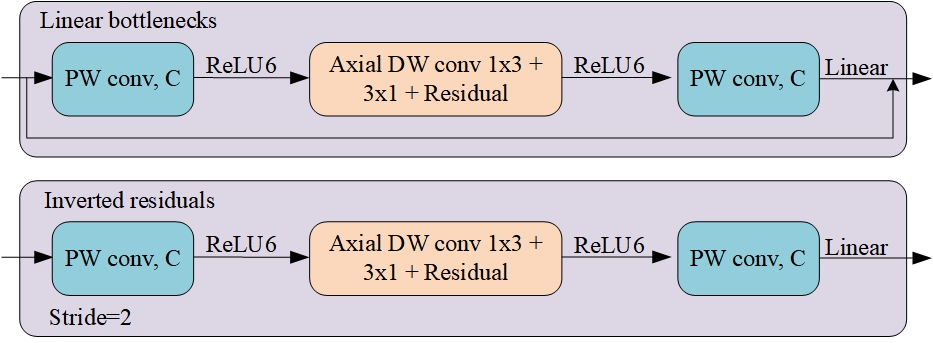
\includegraphics[width=0.7\linewidth]{picture/LLIE/My Architecture/Base module}
		%		%\captionsetup{font=scriptsize}
		%		\caption{Linear bottlenecks 和 Inverted residuals}
		%		\label{fig: Base module}	
		%	\end{figure}
	
	%	现有的方法仍有很大的改进空间,例如如何在提高亮度的同时消除产生的噪声,如何避免颜色失真现象等。一些现有的方法可以有效地解决一个问题,但往往会忽略了其他问题。不同的方法在不同的数据集上往往具有不同的优势,即在不同的评估标准下有不同的优势,如图\ref{fig: VE-LOL-L Visual}展示了不同算法在VE-LOL-L数据集下的可视化结果。
	%	
	%	\begin{figure}[htbp]
		%		\centering
		%		\begin{subfigure}{0.17\columnwidth}
			%			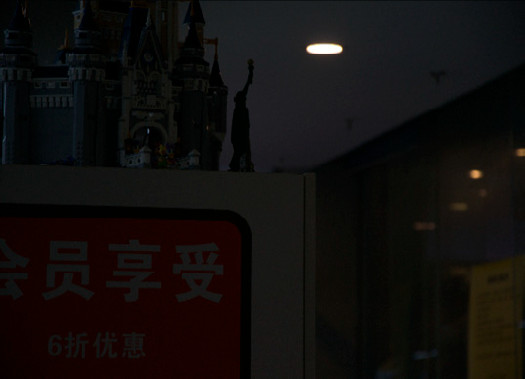
\includegraphics[width=\linewidth]{picture/LLIE/VE-LOL-L/input}
			%			\captionsetup{font=scriptsize}
			%			\caption*{input \\ \quad }
			%			\label{fig: input}
			%		\end{subfigure}
		%		\begin{subfigure}{0.17\columnwidth}
			%			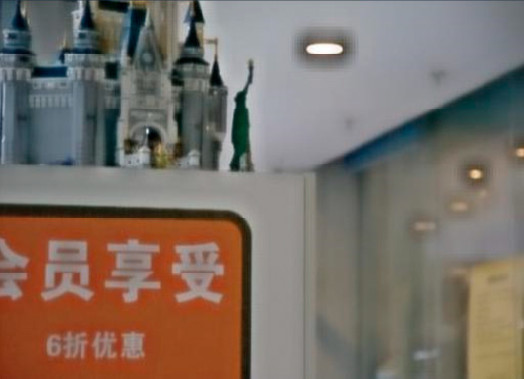
\includegraphics[width=\linewidth]{picture/LLIE/VE-LOL-L/LLNet}
			%			\captionsetup{font=scriptsize}
			%			\caption*{LLNet \\ (2017)}
			%			\label{fig: LLNet_VE_LOL}	
			%		\end{subfigure}
		%		\begin{subfigure}{0.17\columnwidth}
			%			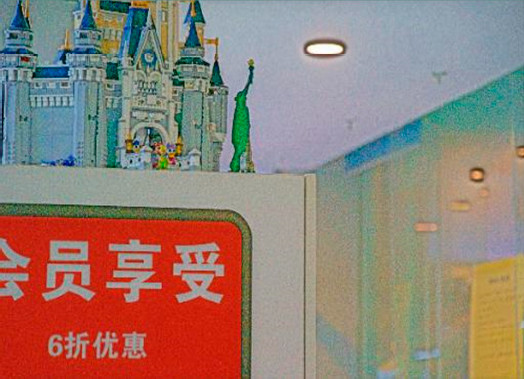
\includegraphics[width=\linewidth]{picture/LLIE/VE-LOL-L/RetinexNet}
			%			\captionsetup{font=scriptsize}
			%			\caption*{RetinexNet \\ (2018)}
			%			\label{fig: RetinexNet_VE_LOL}	
			%		\end{subfigure}
		%		\begin{subfigure}{0.17\columnwidth}
			%			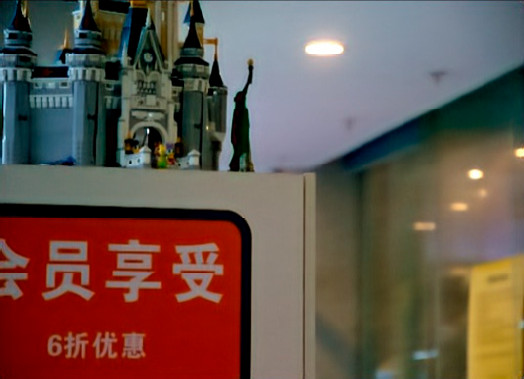
\includegraphics[width=\linewidth]{picture/LLIE/VE-LOL-L/MBLLEN}
			%			\captionsetup{font=scriptsize}
			%			\caption*{MBLLEN \\ (2018)}
			%			\label{fig: MBLLEN_LOL}	
			%		\end{subfigure}
		%		\begin{subfigure}{0.17\columnwidth}
			%			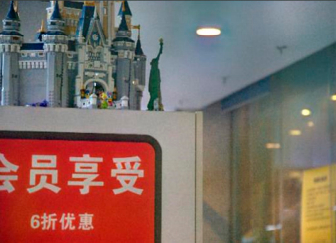
\includegraphics[width=\linewidth]{picture/LLIE/VE-LOL-L/EnlightenGAN}
			%			\captionsetup{font=scriptsize}
			%			\caption*{EnlightenGAN \\ (2019)}
			%			\label{fig: EnlightenGAN_VE_LOL}	
			%		\end{subfigure}
		%		\begin{subfigure}{0.17\columnwidth}
			%			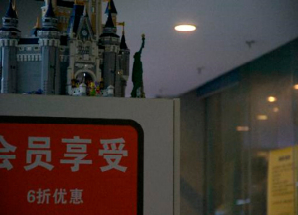
\includegraphics[width=\linewidth]{picture/LLIE/VE-LOL-L/RRDNet}
			%			\captionsetup{font=scriptsize}
			%			\caption*{RRDNet \\ (2020)}
			%			\label{fig: RRDNet_VE_LOL}	
			%		\end{subfigure}
		%		\begin{subfigure}{0.17\columnwidth}
			%			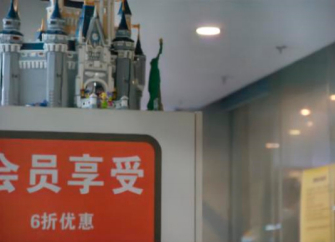
\includegraphics[width=\linewidth]{picture/LLIE/VE-LOL-L/DRBN}
			%			\captionsetup{font=scriptsize}
			%			\caption*{DRBN \\ (2020)}
			%			\label{fig: DRBN_VE_LOL}	
			%		\end{subfigure}
		%		\begin{subfigure}{0.17\columnwidth}
			%			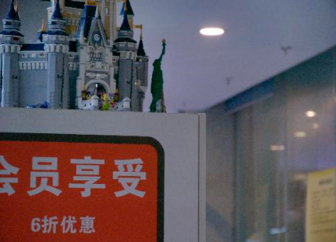
\includegraphics[width=\linewidth]{picture/LLIE/VE-LOL-L/Zero-DCE++}
			%			\captionsetup{font=scriptsize}
			%			\caption*{Zero-DCE++ \\ (2021)}
			%			\label{fig: Zero-DCE++}	
			%		\end{subfigure}
		%		\begin{subfigure}{0.17\columnwidth}
			%			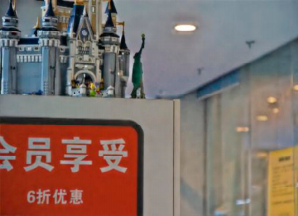
\includegraphics[width=\linewidth]{picture/LLIE/VE-LOL-L/KinD++}
			%			\captionsetup{font=scriptsize}
			%			\caption*{KinD++ \\ (2021)}
			%			\label{fig: KinD++}	
			%		\end{subfigure}
		%		\begin{subfigure}{0.17\columnwidth}
			%			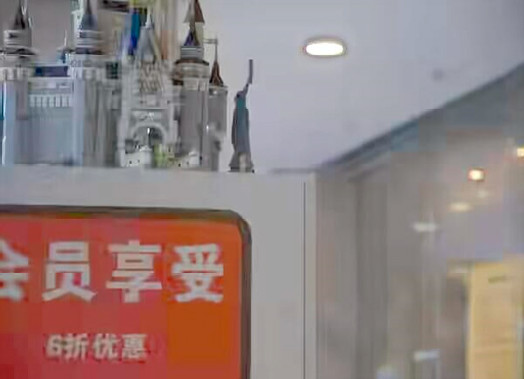
\includegraphics[width=\linewidth]{picture/LLIE/VE-LOL-L/URetinexNet}
			%			\captionsetup{font=scriptsize}
			%			\caption*{URetinexNet \\ (2022)}
			%			\label{fig: URetinexNet}	
			%		\end{subfigure}
		%		\caption{
			%			\label{fig: VE-LOL-L Visual} 
			%			不同算法对从 VE-LOL-L 数据集采样的低照度图像的可视化结果。 
			%		}
		%	\end{figure}
	%	
	%	近年来,基于深度学习的低光图像增强(LLIE)技术取得了显著成就,它使用神经网络来学习从低光图像到自然光图像的映射。与传统方法相比,基于深度学习的解决方案在准确性、鲁棒性和处理速度方面表现更优,因此受到了广泛关注。特别是卷积神经网络(CNN)在多个计算机视觉任务中展现出卓越的性能。CNN通过利用注意力机制和\cite{yang2021locally, zhang2020attention}上下文信息,能够从原始图像中有效提取多尺度特征\cite{li2018multi, zamir2020learning}。在这些成果的推动下,基于CNN的低光图像增强方法得到了持续发展。例如,一种基于CNN的自适应低光图像增强框架\cite{li2020visual}显著提升了图像的对比度、颜色和细节信息。然而,现有的基于CNN的方法大多集中于图像亮度、纹理和颜色的恢复,对于局部光照不均匀、颜色信息和细节信息的丢失问题,仍存在过增强或增强不足的挑战。
	%	
	%	现有的方法可能无法在极暗或极亮的区域恢复图像边缘细节\cite{xu2023low},如图\ref{fig: SNR (CVPR 2022)}和图\ref{fig: SMG-LLIE}所示,暗区结构细节模糊。同时,当物体边缘不清晰时,像素级损失往往会模糊边缘,破坏图像细节。而加入边缘先验可以降低优化外观重构时的不适定程度。人类视觉系统对边缘高度敏感,保留结构信息对图像重建任务的性能至关重要。定义边缘可以通过学习区分黑暗区域的不同物体来指导增强过程,而不仅仅是识别低光区域。通过保留图像中的结构属性,这使得物体之间的可见性更好。
	%	
	%	\begin{figure}[htb]
		%		\centering
		%		\begin{subfigure}{0.45\columnwidth}
			%			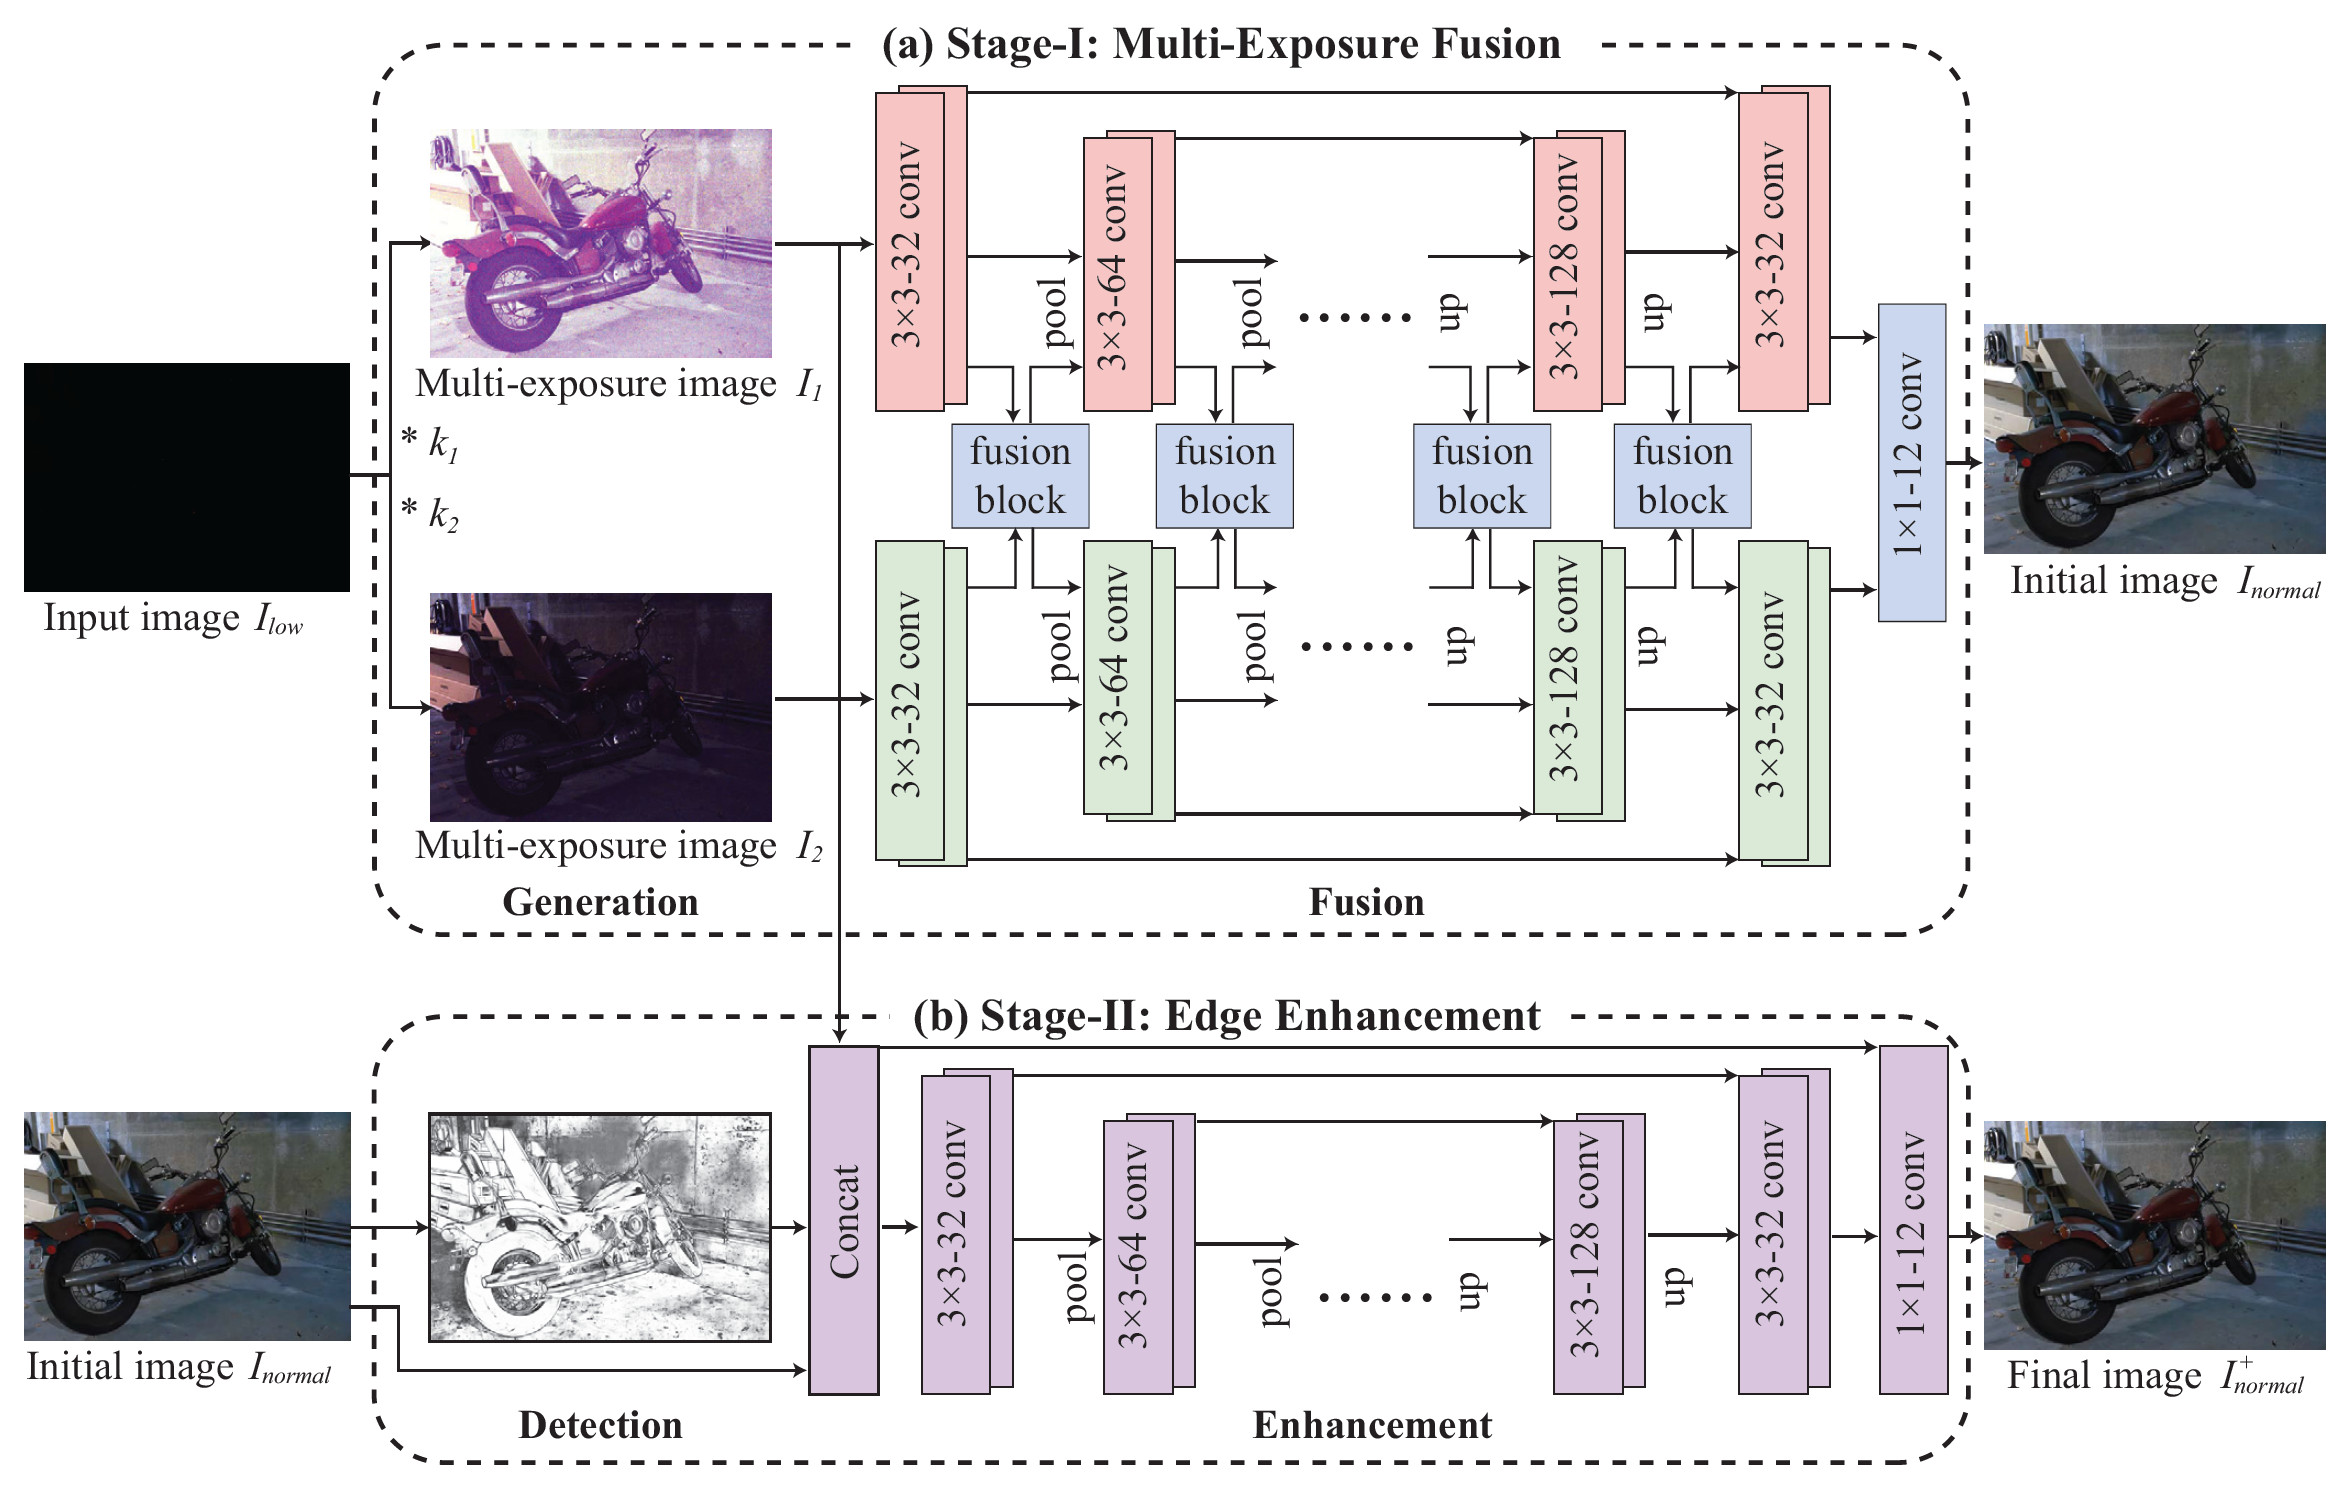
\includegraphics[width=\linewidth]{picture/LLIE/EEMEFN/EEMEFN framework}
			%			\captionsetup{font=scriptsize}
			%			\caption{\label{fig: EEMEFN}
				%				该 LLIE 结构源自\cite{zhu2020eemefn},如其 Multi-Exposure Fusion 部分采用多曝光融合结构,与由 Initial image 生成的边缘图进行 Concat, 后续通过一个 U-Net 网络进一步恢复图像。}
			%		\end{subfigure}
		%		\begin{subfigure}{0.45\columnwidth}
			%			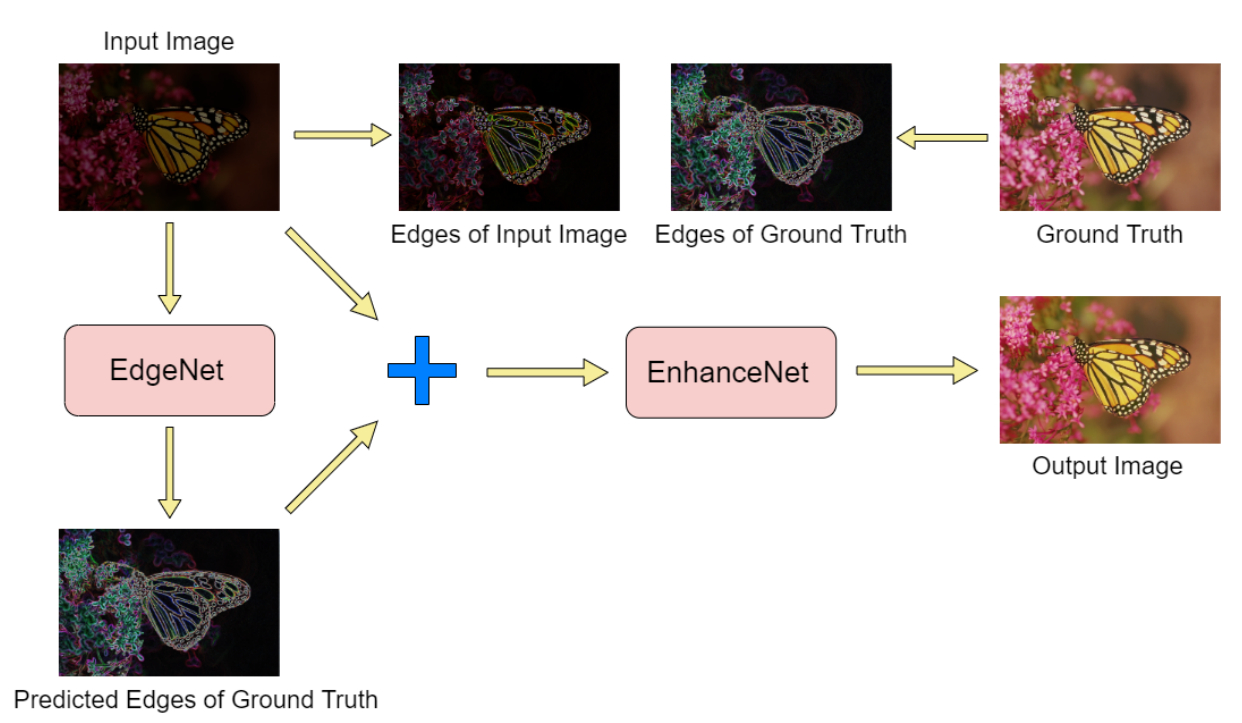
\includegraphics[width=\linewidth]{picture/LLIE/EdgeNet/Archtecture workflow}
			%			\captionsetup{font=scriptsize}
			%			\caption{\label{fig: EdgeNet} 
				%				该 LLIE 结构源自\cite{rana2021edge}使用 EdgeNet 首先从低光图像中过滤边缘,EnhanceNet 反复使用上采样和下采样块的组合,从局部到全局逐渐提取特征,并消除伪影和噪声。}
			%		\end{subfigure}
		%		\caption{
			%			\label{fig: Traditional Architecture}
			%			边缘图像指导低光图像增强的传统架构。
			%		}
		%	\end{figure}
	%	
	%	\begin{figure}[htb]
		%		\centering 
		%		\begin{subfigure}{0.8\columnwidth}
			%			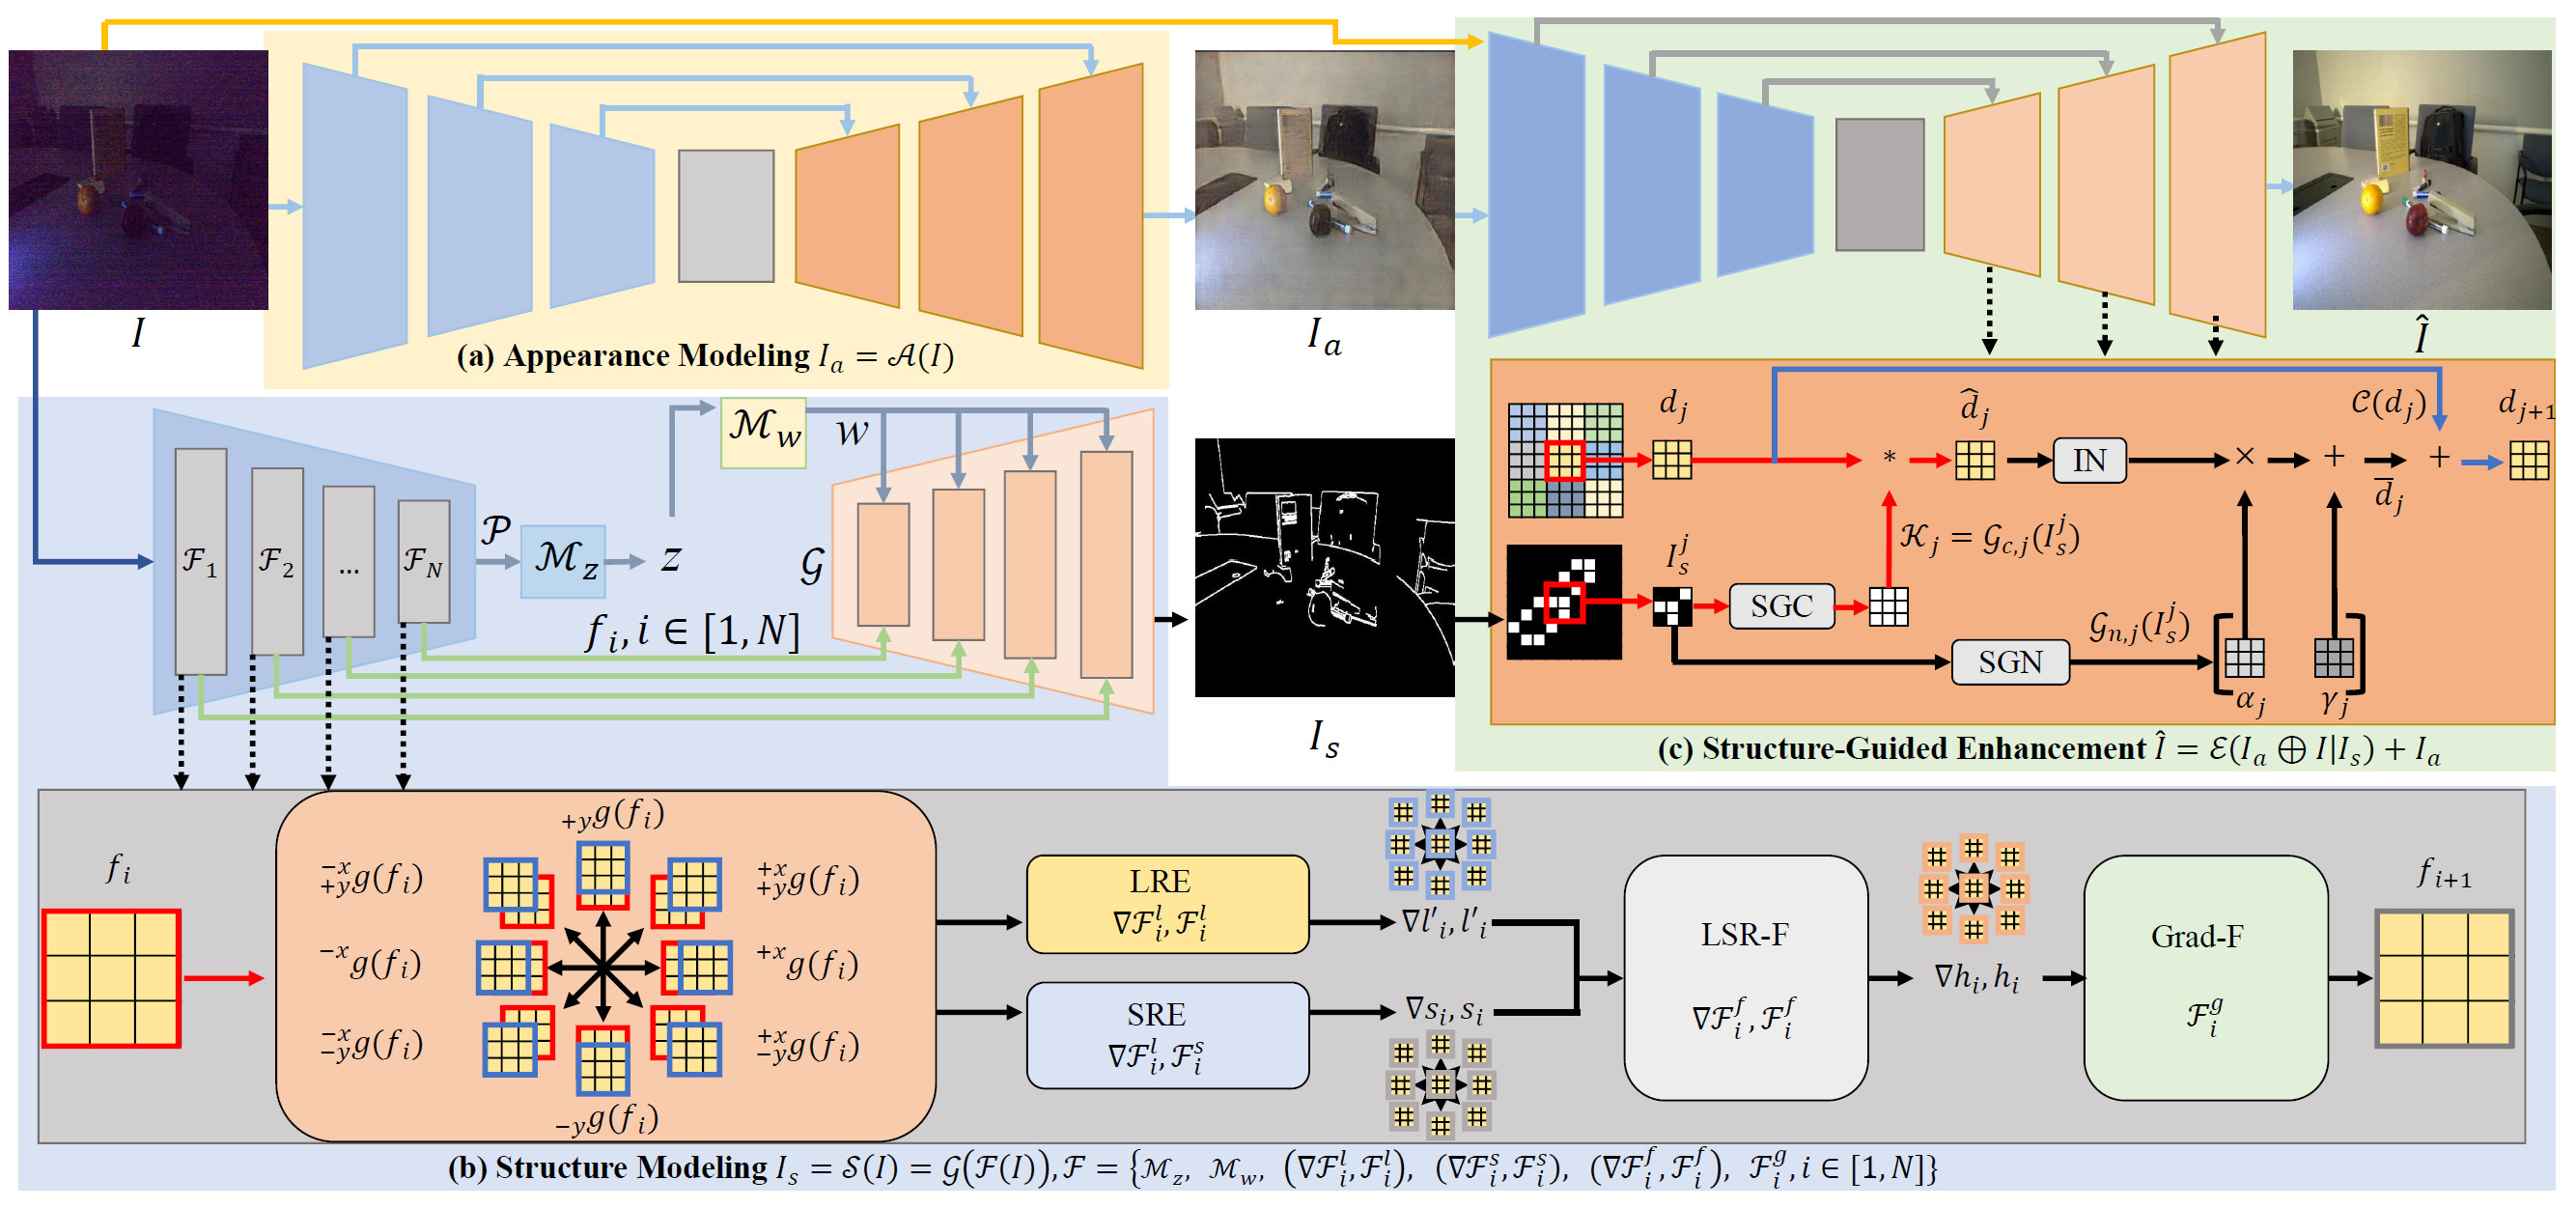
\includegraphics[width=\columnwidth]{picture/LLIE/Structure Modeling and Guidance/Overview}
			%			\captionsetup{font=scriptsize}
			%			\caption{该 LLIE 结构源自\cite{xu2023low},其提出一种基于 GAN Loss 的模型去对结构信息建模,通过获得的结构信息指导增强。}
			%			\label{fig: SMG-LLIE Architecture}
			%		\end{subfigure}
		%		\caption{
			%			\label{fig: SMG-LLIE Overview} 
			%			边缘图像指导低光图像增强的最新架构(CVPR 2023)。
			%		}
		%	\end{figure}
	%	
	%	\begin{figure}[htb]
		%		\centering
		%		\begin{subfigure}{0.25\columnwidth}
			%			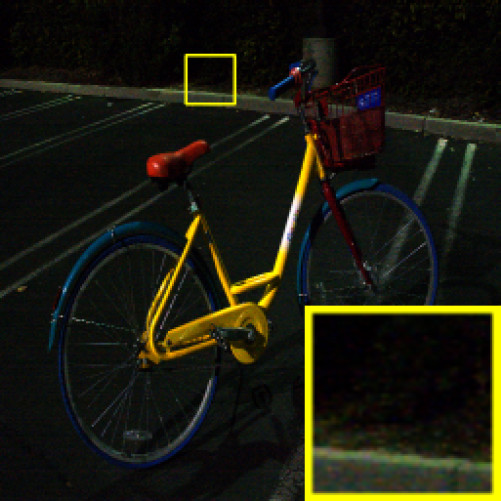
\includegraphics[width=\linewidth]{picture/LLIE/Structure Modeling and Guidance/Input}
			%			\captionsetup{font=scriptsize}
			%			\caption{Input}
			%			\label{fig: Input}
			%		\end{subfigure}
		%		\begin{subfigure}{0.25\columnwidth}
			%			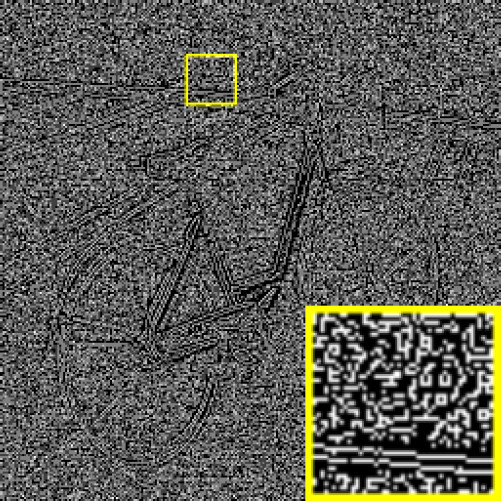
\includegraphics[width=\linewidth]{picture/LLIE/Structure Modeling and Guidance/Structure of (a)}
			%			\captionsetup{font=scriptsize}
			%			\caption{Structure of (a)}
			%			\label{fig: Structure of (a)}	
			%		\end{subfigure}
		%		\begin{subfigure}{0.25\columnwidth}
			%			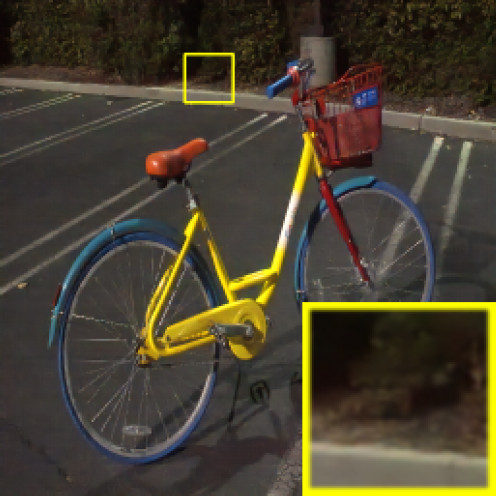
\includegraphics[width=\linewidth]{picture/LLIE/Structure Modeling and Guidance/SNR (CVPR 2022)}
			%			\captionsetup{font=scriptsize}
			%			\caption{SNR (CVPR 2022)}
			%			\label{fig: SNR (CVPR 2022)}	
			%		\end{subfigure}
		%		\begin{subfigure}{0.25\columnwidth}
			%			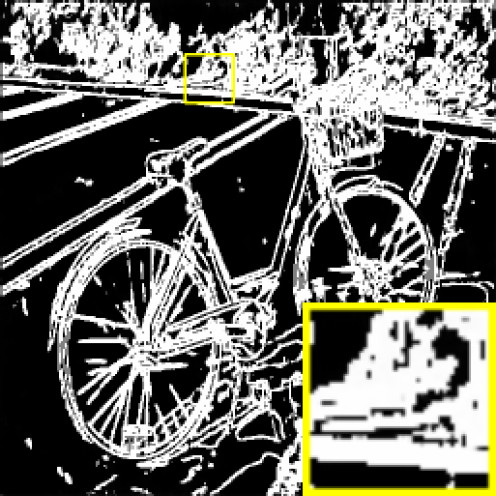
\includegraphics[width=\linewidth]{picture/LLIE/Structure Modeling and Guidance/Structure Modeling}
			%			\captionsetup{font=scriptsize}
			%			\caption{Structure Modeling}
			%			\label{fig: Structure Modeling}
			%		\end{subfigure}
		%		\begin{subfigure}{0.25\columnwidth}
			%			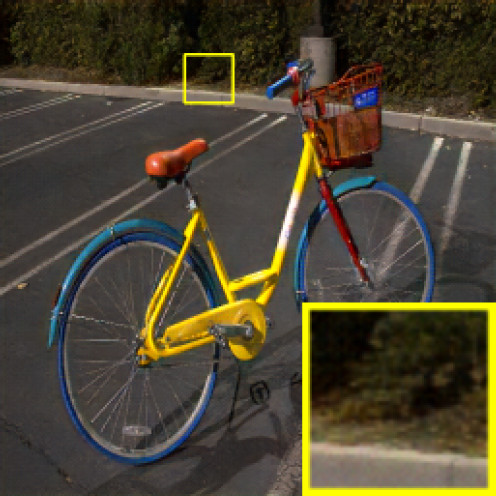
\includegraphics[width=\linewidth]{picture/LLIE/Structure Modeling and Guidance/Ours}
			%			\captionsetup{font=scriptsize}
			%			\caption{SMG-LLIE}
			%			\label{fig: SMG-LLIE}
			%		\end{subfigure}
		%		\begin{subfigure}{0.25\columnwidth}
			%			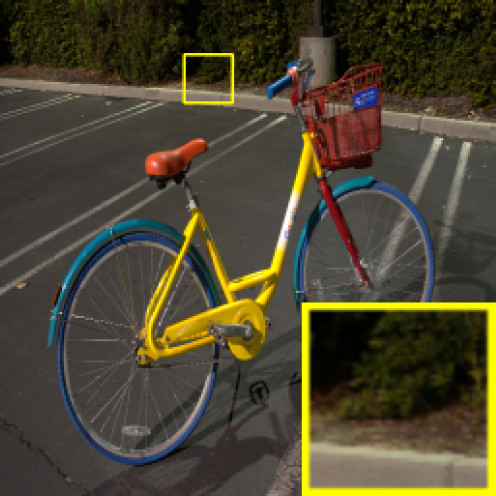
\includegraphics[width=\linewidth]{picture/LLIE/Structure Modeling and Guidance/Ground Truth}
			%			\captionsetup{font=scriptsize}
			%			\caption{Ground Truth}
			%			\label{fig: Ground Truth}
			%		\end{subfigure}
		%		\caption{
			%			\label{fig: Structural Information}
			%			SID-sRGB\cite{chen2018learning}中一张低光图片, 通过SOTA方法 (c) 和\cite{xu2023low}提出的方法 (e)增强。作者的方法可以从输入的图像中合成结构图(d),使细节更清晰,对比度更清晰,颜色更鲜艳。虽然(c)的 PSNR 为 28.17,但其 SSIM 低为 0.75。作者的方法在dB和SSIM\cite{wang2004image}的得分都很高,分别为28.60 dB 和 0.80。
			%		}
		%	\end{figure}
	%	
	%	基于这个问题,即\textbf{如何更好的使用边缘图来“指导”低光图像的恢复?}我们对此进行了相关文献调研。其中,一类方法(如图\ref{fig: Traditional Architecture}所示,我们称之为传统架构)是采用边缘检测思想来引导低光图像增强,其策略是将边缘图与\textbf{一张从低光中初步恢复的图像}(后面统一称作初步恢复图像)进行串联,然后通过一个增强网络来实现最终的图像增强\cite{zhu2020eemefn, rana2021edge}。但是我们通过观察这类模型的架构发现其具有以下三个特点:
	%	
	%	\begin{itemize}
		%		\item [(1)] 其恢复结果的质量往往会受到最后的增强网络设计和初步恢复图像所包含特征与真实图像特征之间的相似度的影响。
		%		
		%		\item [(2)] 边缘图的准确性会极大影响最终的恢复结果,直接从低光图像中获取边缘图具有一定的挑战性。
		%		
		%		\item [(3)] 边缘图与初步恢复图像之间多采用串联方式输入卷积以获得最终增强结果。
		%	\end{itemize}
	%	
	%	传统架构存在一定的局限性,虽然采用了边缘结构信息增强低光图像,但是无法很好的利用边缘信息语义指导恢复低光图像,需要在现有的直接串联方法的基础上进行改进。此外,从低光照中的图片很难提取到好的结构信息,如何设计更好的边缘网络从低光图像中提取出接近 GT 边缘图的结果是我们需要考虑的问题。
	%	
	%	作者\cite{xu2023low}提出了一种基于结构先验的图像增强方式,以更好的从低光图像中提取到更有效的边缘信息并用于指导图像增强。从图\ref{fig: Structural Information}和\ref{fig: LLI Structure Information}中可以看到边缘图和LBP图\cite{pietikainen2010local}所反映结构信息具有明显的区别,边缘信息能反映更多的细节信息。我们不难发现,相较于LBP,图像边缘图仅保留了很少的数据量,其剔除了不相关的信息,保留了图像重要的结构属性。人类视觉系统对边缘高度敏感,保留结构信息对图像重建任务的性能至关重要。定义边缘可以通过学习区分黑暗区域的不同物体来指导增强过程,而不仅仅是识别低光区域。通过保留图像中的结构属性,这使得物体之间的可见性更好。
	
	\subsection{研究内容}
	
	综上所述,本研究旨在实现以下明确的研究目标
	
	%\footnote{在对Xu等人\cite{xu2023low}的模型(参见图\ref{fig: SMG-LLIE Architecture})进行深入分析后,本研究旨在通过采用与原作者不同的方法论来实现若干具体目标,并力求在关键评价指标上超越原模型的性能。具体而言,本研究的核心目标包括:首先,在目标(1)和目标(2)的框架内,探索与Xu等人不同的优化策略;其次,这些优化策略应致力于提升模型的整体性能,目的在于在关键评价指标上实现超越原作者的成果。通过这种方法,本研究不仅旨在增强现有模型的能力,同时也寻求对该领域的理论和实践知识做出贡献。}:
	
	\begin{itemize}
		\item [(1)] \textbf{边缘网络的开发:} 设计并构建一个创新的边缘网络,其核心功能是从低光照图像中直接提取边缘结构图。该网络生成的结构图应与地面真实(GT)生成的边缘结构图具有高度的相似性,从而确保准确性和可靠性。
		
		\item [(2)] \textbf{多通道低光图像增强模型:} 开发一个基于HSV通道的低光照图像增强模型。该模型应专注于从低光条件下的图像中恢复亮度、对比度和颜色,以提高整体图像质量。
		
		\item [(3)] \textbf{基于边缘语义信息的增强网络模型:} 在现有的直接串联方法基础上,进行创新性改进,构建一种更有效利用边缘语义信息的增强网络模型。目的在于通过这种改进,进一步提升图像增强过程中边缘结构的利用效率和效果。
	\end{itemize}
	
	通过实现这些目标,本研究期望对低照度图像处理领域的理论与实践作出贡献,特别是在图像边缘结构的提取和利用方面。
	
	%	\section{摘要}
	%	
	%		低光图像增强(LLIE)旨在增强图像亮度并恢复低光图像细节。然而,现有基于深度学习的LLIE模型仍面临诸如信息丢失、细节恢复不足、噪声、色差和细节失真等挑战,导致无法准确恢复低光图像(LLI)中的暗部细节,且模型往往过于复杂且存在冗余。为了解决这些问题,本文提出了一种简单而有效的LLIE模型,称为上下文网络(xxx-Net)。该模型由两个核心部分组成:1) 基于U-Net架构的编码器和解码器,用于处理图像的整体结构;2) 位于模型中心的BottleNeck块,由Swin Transformer块组成,用于捕获低光图像的全局上下文信息。此外,我们还引入了即插即用的Cbam块,以学习和强调低光图像中的局部细节。通过大量实验,我们证明了xxx-Net在恢复低光图像的暗部区域方面具有出色的性能,同时具有较少的参数和更快的推理速度,从而在低光图像增强任务中取得了显著的进步。
	%	
	%	\section{引言}
	%		
	%		低光图像增强(Low-Light Image Enhancement, LLIE)是视觉监控、自动驾驶和计算摄影等领域的重要应用之一。低光条件下拍摄的照片常常会遭受多种退化现象,如低对比度、可见度不足、噪声和色彩失真,这些问题不仅影响视觉感知,还会干扰后续的高级图像处理任务。因此,低光图像增强是图像处理领域的一个关键任务,旨在提升低光环境下拍摄图像的视觉质量。近年来,该领域的发展主要受到深度学习技术的驱动,涉及多种学习策略、网络架构、损失函数和训练数据集的运用。然而,在低光图像中恢复照度并精确恢复极暗区域的细节信息依然是一项充满挑战的任务。
	%		%尤其在智能手机摄影领域,由于相机光圈大小、实时处理需求和存储限制,低光环境下的图像拍摄面临着显著挑战。
	%		为应对这一挑战,研究人员提出了众多LLIE方法,包括传统方法和基于深度学习的方法。
	%		
	%		
	%		%介绍传统的低光图像增强方法
	%		传统的低光图像增强技术,如基于直方图均衡化\cite{ji1994adaptive}和Retinex理论\cite{land1965, land1977retinex, jobson1997properties}的方法,能在一定程度上提升图像的视觉质量。这些方法通常依赖于各种图像先验来构建模型,以逆向恢复退化的图像。然而,尽管这些传统技术能够增强图像的整体对比度,它们往往也会加剧背景噪声的对比度,同时减弱有价值的图像细节的对比度,从而影响最终的视觉效果。%Retinex算法旨在消除图像照度分量的干扰并还原图像真实色彩,但通常忽略噪声问题,可能导致增强结果中噪声的保留或放大,并且其复杂的优化过程增加了模型的复杂度。	
	%		%传统的低光增强方法,如基于直方图均衡\cite{ji1994adaptive}和 Retinex\cite{land1965, land1977retinex, jobson1997properties}的方法,直方图均衡化重新调整图像的直方图分布,一方面增加了图像的全局对比度,另一方面使得亮度在整个图像的分布更加均匀。直方图均衡化的方法非常快速有效,并且是一个可逆操作,但缺点在于其不加选择地处理数据,可能增加背景噪声的对比度,同时降低有用的图像内容的对比度,导致视觉效果欠佳。此外,该方法也无法适用于复杂多变的低光照场景。Retinex 算法的核心思想是消除源图像照度分量干扰,依据反射分量信息还原图像真实色彩。基于 Retinex 的方法能够很大程度改善图像质量,但在应用的过程中仍存在不可忽视的缺点。例如,其通常忽略噪声问题,可能导致增强结果中噪声的保留或放大;有效的先验或正则化的选择具有挑战性,不准确的先验可能导致伪影和颜色偏差;此外,这些方法的复杂优化过程也导致最终的模型较为复杂。
	%		近年来,基于深度学习的低光图像增强技术取得了显著成就,其通过设计各种模块和损失函数来学习从低光图像到正常光图像的映射。由于深度学习方法强大的学习能力,往往能够产生更好的细节恢复结果。CNN通过利用注意力机制\cite{yang2021locally,zhang2020attention}和上下文信息,能够从原始图像中有效提取局部特征\cite{jain1991unsupervised, lowe2004distinctive, ojala2002multiresolution}。在低光图像中,亮度较低、对比度较弱的区域之间存在一定的关联性和相互作用,如果模型能够捕获全局光照,将有助于恢复图像的整体亮度和对比度\cite{chen2018learning, wang2013naturalness}\footnote{Retinex 理论的一个关键思想是图像的颜色和亮度感知取决于全局光照条件,因此捕获和调整全局光照信息对于图像增强和恢复至关重要。}。在图像处理领域,尤其是在低光图像恢复和增强方面,保持图像的结构完整性是一个重要的挑战。Fu 等人\cite{fu2016weighted}引入了一种加权变分模型,通过边缘感知权重来保持图像的结构完整性,从而在增强过程中保持边缘和细节信息。随后,Wang 等人\cite{wang2018esrgan}在其提出的 ESRGAN 模型中强调了集成全局和局部特征的重要性,包括保持边缘和纹理细节的完整性,以增强图像的感知质量。最近,Xu\cite{xu2020learning}提出了一种基于深度学习的方法,通过分解和增强来恢复低光图像,其中在分解阶段保持了图像的结构信息,包括边缘和纹理细节,这对于后续的增强阶段至关重要。因此,即使在低光条件下,对象的轮廓和边缘仍然是重要的视觉特征,捕获这些全局的边缘信息对于保持图像的结构完整性至关重要。
	%		
	%		在低光条件下捕获和恢复图像中的纹理和模式是图像增强领域的一项重要挑战。Loh等人\cite{loh2019getting}通过对低光照图像的特性进行研究,强调了在低光条件下保持图像纹理和模式的重要性。进一步地,Jiang 等人\cite{jiang2021enlightengan}提出了一种基于生成对抗网络的方法,有效地恢复了低光图像中的细节,包括难以辨识的纹理和模式。同样,Lv 等人\cite{lv2018mbllen}通过卷积神经网络增强了低光图像和视频,专注于恢复纹理和模式的细节,从而提供更丰富的图像内容。因此,尽管低光图像中的纹理和模式可能难以辨识,但它们对于理解图像内容仍然非常重要。理解图像内容的关键在于识别不同对象和场景元素之间的空间关系。Wei 等人\cite{wei2018deep}提出的深度 Retinex 分解方法通过在特征提取过程中考虑全局依赖关系来进一步提高低光图像的质量。
	%		
	%		在低光图像增强领域,现有的基于 CNN 的方法面临着一些挑战。Hao等人\cite{hao2020low}提出了一种半解耦分解的方法来增强低光图像,该方法旨在解决局部光照不均匀的问题,并改善颜色和细节的恢复。他们指出,传统的基于 CNN 的方法可能无法有效处理这些问题。同样,Ravirathinam 等人\cite{ravirathinam2021c}提出了一种多上下文特征提取模块,该模块专注于捕获高级上下文特征、结构相似性和局部信息。他们的研究指出,仅依赖局部感受野的 CNN 方法可能难以充分利用全局上下文信息。此外,Xu等人\cite{xu2021novel}提出了一种多尺度特征引导的注意力机制,以更多地关注那些黑暗和信息丰富的区域。他们强调,单一尺度的 CNN 方法可能受到感受野大小的限制,导致在处理细节丢失和局部光照不均匀问题时效果不佳。因此,开发能够克服这些限制并有效提升低光图像质量的深度学习模型仍然是一个重要的研究方向。
	%		
	%%		在低光图像中亮度较低、对比度较弱的区域之间存在一定的关联性和相互作用,如果模型能够捕获全局光照有助于恢复图像的整体亮度和对比度。
	%%		
	%%		同样,即使在低光条件下,对象的轮廓和边缘仍然是重要的视觉特征。捕获这些长距离的边缘信息对于保持图像的结构完整性至关重要。
	%%		
	%%		纹理和模式,低光图像中的纹理和模式可能难以辨识,但它们对于理解图像内容仍然很重要。长距离特征可以帮助模型识别和恢复这些纹理和模式。
	%%		
	%%		不同对象和场景元素之间的空间关系是理解图像的关键。在低光图像中,捕获这些长距离的上下文关系对于正确的解释图像至关重要。
	%%		
	%%		然而,现有的基于CNN的方法在处理局部光照不均匀、颜色信息和细节信息丢失问题时,仍存在过增强或增强不足的挑战,并且增强结果受到感受野大小的限制。
	%
	%
	%%		
	%		%近年来,基于深度学习的低光图像增强 (LLIE) 方法取得了显著的成功。与传统方法相比,基于深度学习的解决方案在准确性、鲁棒性和速度方面表现更佳,因此受到了越来越多的关注。近年来,基于深度学习的低光图像增强 (LLIE) 技术取得了显著成就,它使用神经网络来学习从低光图像到自然光图像的映射。与传统方法相比,基于深度学习的解决方案在准确性、鲁棒性和处理速度方面表现更优,因此受到了广泛关注。特别是卷积神经网络(CNN)在多个计算机视觉任务中展现出卓越的性能。CNN 通过利用注意力机制和\cite{yang2021locally, zhang2020attention}上下文信息,能够从原始图像中有效提取多尺度特征\cite{li2018multi, zamir2020learning}。在这些成果的推动下,基于 CNN 的低光图像增强方法得到了持续发展。此外,现有的基于 CNN 的方法大多集中于图像亮度、纹理和颜色的恢复,对于局部光照不均匀、颜色信息和细节信息的丢失问题,仍存在过增强或增强不足的挑战,同时增强结果受到感受野大小的限制,但通过增大卷积核以及多次卷积的方法进行卷积又会增加模型的复杂度。
	%		
	%		为了解决这些问题,我们提出了一种新颖的方法(方法名待定)。受到ULite\cite{dinh20231m}中深度可分离卷积的启发,我们将U-Net网络中的卷积改为轴向深度可分离卷积,以减少模型冗余同时保持增强效果。此外,我们借鉴Swin-Unet\cite{cao2022swin}在BottleNeck中使用连续的Swin Transformer块以捕获图像全局特征,相较于传统的Transformer块,Swin Transformer能够减少参数量和模型复杂度。通过以上改进,我们的方法能够有效提升低光图像的视觉质量,同时保持较低的计算复杂度,具有实际应用的潜力。
	%		
	%		%低光图像增强结果也会受到低光区域的形状和大小的影响,在深度学习的框架下,卷积神经网络(CNN)通过分层的卷积操作,逐步提取并加工图像的局部特征\cite{jain1991unsupervised, lowe2004distinctive, ojala2002multiresolution},而难以获取图像中的长距离特征,进而导致结果增强过或不足,为了解决这些问题,\textcolor{red}{我们提出了一种方法(方法名待定)}。我们受到ULite\cite{dinh20231m}中深度可分离卷积的启发,将原有的 U-Net 网络中的卷积改为轴向深度可分离卷积,通过这种方式在不损害增强效果的情况下,减少模型冗余。此外,我们借鉴于 Swin-Unet\cite{cao2022swin} 在 BottleNeck 中使用连续的 Swin Transformer 块以捕获图像长距离特征。相较于使用 Transformer 块,使用 Swin Transformer 能够减少参数量和模型复杂度。
	%		
	%%		现有的方法仍有很大的改进空间,例如如何在提高亮度的同时消除产生的噪声,如何避免颜色失真现象等。一些现有的方法可以有效地解决一个问题,但往往会忽略了其他问题。不同的方法在不同的数据集上往往具有不同的优势,即在不同的评估标准下有不同的优势,如图.\ref{fig: VE-LOL-L Visual}展示了不同算法在 VE-LOL-L 数据集下的可视化结果。
	%%
	%%		\begin{figure}[htbp]
		%%			\centering
		%%			\setlength{\abovecaptionskip}{-0.05cm}
		%%			\begin{subfigure}{0.17\columnwidth}
			%%				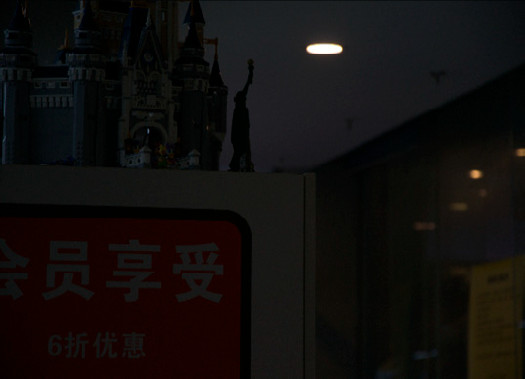
\includegraphics[width=\linewidth]{picture/LLIE/VE-LOL-L/input}
			%%				\captionsetup{font=scriptsize}
			%%				\caption*{input \\ \quad }
			%%				\label{fig: input}
			%%			\end{subfigure}
		%%			\begin{subfigure}{0.17\columnwidth}
			%%				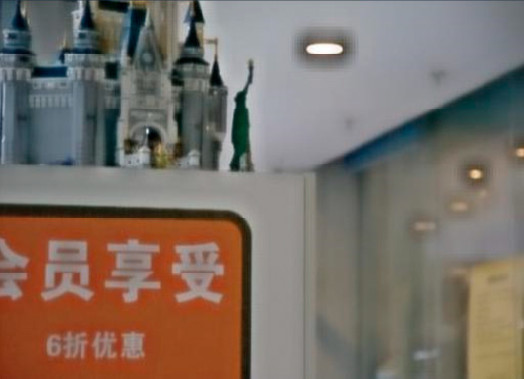
\includegraphics[width=\linewidth]{picture/LLIE/VE-LOL-L/LLNet}
			%%				\captionsetup{font=scriptsize}
			%%				\caption*{LLNet \\ (2017)}
			%%				\label{fig: LLNet_VE_LOL}	
			%%			\end{subfigure}
		%%			\begin{subfigure}{0.17\columnwidth}
			%%				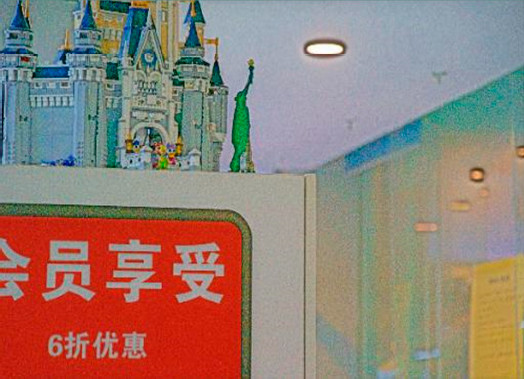
\includegraphics[width=\linewidth]{picture/LLIE/VE-LOL-L/RetinexNet}
			%%				\captionsetup{font=scriptsize}
			%%				\caption*{RetinexNet \\ (2018)}
			%%				\label{fig: RetinexNet_VE_LOL}	
			%%			\end{subfigure}
		%%			\begin{subfigure}{0.17\columnwidth}
			%%				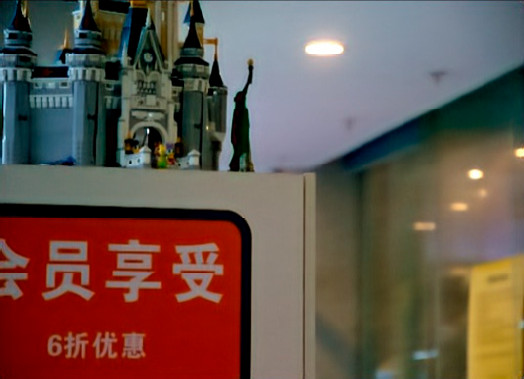
\includegraphics[width=\linewidth]{picture/LLIE/VE-LOL-L/MBLLEN}
			%%				\captionsetup{font=scriptsize}
			%%				\caption*{MBLLEN \\ (2018)}
			%%				\label{fig: MBLLEN_LOL}	
			%%			\end{subfigure}
		%%			\begin{subfigure}{0.17\columnwidth}
			%%				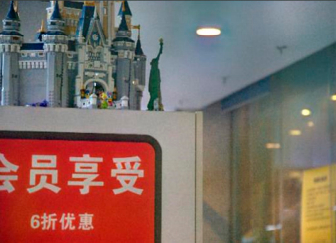
\includegraphics[width=\linewidth]{picture/LLIE/VE-LOL-L/EnlightenGAN}
			%%				\captionsetup{font=scriptsize}
			%%				\caption*{EnlightenGAN \\ (2019)}
			%%				\label{fig: EnlightenGAN_VE_LOL}	
			%%			\end{subfigure}
		%%			\begin{subfigure}{0.17\columnwidth}
			%%				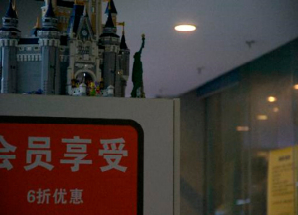
\includegraphics[width=\linewidth]{picture/LLIE/VE-LOL-L/RRDNet}
			%%				\captionsetup{font=scriptsize}
			%%				\caption*{RRDNet \\ (2020)}
			%%				\label{fig: RRDNet_VE_LOL}	
			%%			\end{subfigure}
		%%			\begin{subfigure}{0.17\columnwidth}
			%%				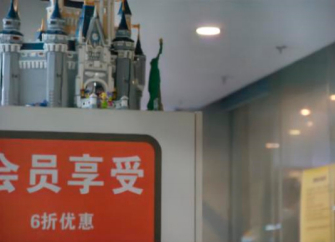
\includegraphics[width=\linewidth]{picture/LLIE/VE-LOL-L/DRBN}
			%%				\captionsetup{font=scriptsize}
			%%				\caption*{DRBN \\ (2020)}
			%%				\label{fig: DRBN_VE_LOL}	
			%%			\end{subfigure}
		%%			\begin{subfigure}{0.17\columnwidth}
			%%				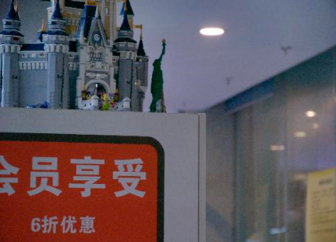
\includegraphics[width=\linewidth]{picture/LLIE/VE-LOL-L/Zero-DCE++}
			%%				\captionsetup{font=scriptsize}
			%%				\caption*{Zero-DCE++ \\ (2021)}
			%%				\label{fig: Zero-DCE++}	
			%%			\end{subfigure}
		%%			\begin{subfigure}{0.17\columnwidth}
			%%				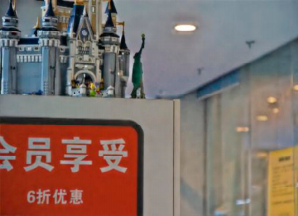
\includegraphics[width=\linewidth]{picture/LLIE/VE-LOL-L/KinD++}
			%%				\captionsetup{font=scriptsize}
			%%				\caption*{KinD++ \\ (2021)}
			%%				\label{fig: KinD++}	
			%%			\end{subfigure}
		%%			\begin{subfigure}{0.17\columnwidth}
			%%				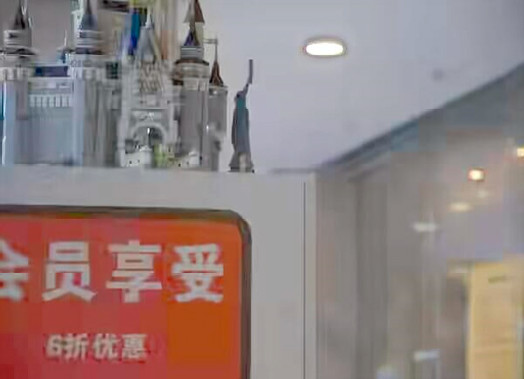
\includegraphics[width=\linewidth]{picture/LLIE/VE-LOL-L/URetinexNet}
			%%				\captionsetup{font=scriptsize}
			%%				\caption*{URetinexNet \\ (2022)}
			%%				\label{fig: URetinexNet}	
			%%			\end{subfigure}
		%%			\caption{
			%%				\label{fig: VE-LOL-L Visual} 
			%%				不同算法对从VE-LOL-L 数据集采样的低照度图像的可视化结果。
			%%			}
		%%		\end{figure}
	%		
	%		
	%		%针对极暗或极亮区域中图像边缘细节恢复的问题,一些研究者提出了在暗区域中加入敏感边缘先验的方法,以降低优化过程中的不适定性,并采用基于编码器-解码器的网络结构和回归损失来执行结构建模。进一步的研究提出了改进的模型,以解决低光图像中局部边缘失真的问题,并对边缘图与弱恢复图的融合策略进行了优化。
	%		
	%		本研究提出了三个主要的创新点:(\textcolor{blue}{若并行架构未实现或性能不佳,则可尝试仅通过CNN分支进行图像的低光恢复,并相应调整创新点,去除并行架构这一创新点。})
	%		\begin{itemize}
		%			\item[$\bullet$]
		%			%首先,提出了一种结合 CNN 和 Transformer 的并行架构用于低光图像增强。我们发现卷积网络通过合理的增加感受野大小,可以有效捕获图像的局部特征,因而我们利用 UNet 网络对低光图像进行弱恢复,使用 Swin Transformer 块捕获图像的长距离特征,最后通过特征融合块将二者特征加以融合。
		%			
		%			首先,提出了一种结合卷积神经网络(CNN)和Transformer的并行架构用于低光图像增强。在该架构中,UNet网络用于捕获图像的局部特征并进行初步恢复,而Swin Transformer块用于捕获图像的长距离特征。最后,通过特征融合块将两者的特征进行融合,以实现更全面的图像增强效果。
		%			\item[$\bullet$] 
		%			%其次,在CNN分支中,提出了一个深度语义模块,融合 Swin Transformer 分支,能有效捕获图像长距离特征;
		%			其次,提出了一个深度语义模块,该模块融合了Swin Transformer分支,使CNN分支能够有效捕获图像的长距离特征。这种设计增强了CNN分支的能力,使其能够更好地理解图像的全局上下文信息。
		%			\item[$\bullet$]
		%			%最后,我们将深度可分离卷积融合进 CNN 分支中,应用于轻量级网络用于提取图像的局部特征;
		%			最后,将深度可分离卷积融合进CNN分支中,应用于轻量级网络用于提取图像的局部特征。这种设计旨在减少模型的参数量和计算复杂度,同时保持对局部特征的有效提取能力。
		%		\end{itemize}
	%		
	%		\section{实验计划}
	%
	%		实验的过程中,确保所有的实验在相同的硬件和软件环境下进行,并且为了确保结果的可靠性,可能需要多次运行实验并取平均值。我们主要基于 PyTorch 进行模型的搭建、训练和评估。基于 scikit-image 库计算 PSNR、SSIM 等评价指标。首先构建 U-Net 基本架构模型,然后实现 Swin Transformer 块中的LocalselfAttention类,PositionEncoding类,PositionEmbedding类。
	%
	%		\subsubsection{Dataset}
	%		
	%		Tab. \ref{tab: Paired_training_datases} 展示了我们在实验中会使用到的低光数据集,这些数据集包含真实数据与合成数据。对于每个数据集,我们需要进行如下操作:
	%		
	%		\begin{itemize}
		%			\item [$\bullet$]
		%			预处理: 确保所有图像都经过相同的预处理步骤,如尺寸调整、归一化等。
		%			
		%			\item [$\bullet$]
		%			分割: 将每个数据集分为训练集、验证集和测试集。
		%		\end{itemize}
	%		
	%		\begin{table}[!htbp]
		%			\centering
		%			\tiny
		%			%\resizebox{\textwidth}{!}{ %按照宽度调整调整表格大小
			%				\begin{tabular}{>{\centering\arraybackslash}m{2.5cm}|c|c|c|c}
				%					
				%					\hline
				%					
				%					\textbf{Name} & \textbf{Number} & \textbf{Format} & \textbf{Real/Syn} & \textbf{Video} \\
				%					
				%					\hline
				%					
				%					LOL\cite{wei2018deep} & 500 & RGB & Real & \\
				%					
				%					SCIE\cite{cai2018learning} & 4,413 & RGB & Real & \\
				%					
				%					VE-LOL-L\cite{jiang2019learning} & 2,500 & RGB & Real+Syn & \\
				%					
				%					\hline
				%					
				%				\end{tabular}
			%				%}
		%			\captionsetup{font=scriptsize} %设置标题字体与表格字体一致
		%			\caption{\label{tab: Paired_training_datases}
			%				Summary of paired training datasets. 'Syn' represents Synthetic.} %表格的标题
		%			
		%		\end{table}
	%		
	%		\subsubsection{Train}
	%		
	%		\begin{itemize}
		%			\item [$\bullet$]
		%			基线模型: 首先,训练基线模型。
		%			
		%			\item [$\bullet$]
		%			消融研究: 接着,训练正常 BottleNeck 的模型,以进行消融实验。
		%		\end{itemize}
	%		
	%		\subsubsection{Performance Evaluation}
	%		
	%		对于每个数据集,使用 Table. \ref{tab: IQA} 指标评估模型性能:
	%		
	%		\begin{table}[!htbp]
		%			\centering
		%			\tiny
		%			%\resizebox{\textwidth}{!}{ %按照宽度调整调整表格大小
			%				\begin{tabular}{>{\centering\arraybackslash}m{5.5cm}|c|c}
				%					
				%					\hline
				%					
				%					\textbf{Name} & \textbf{Abbreviation} & \textbf{Reference} \\
				%					
				%					\hline
				%					
				%					Peak Signal-to-Noise Ratio                           & PSNR    & \checkmark \\
				%					
				%					Structural Similarity Index                          & SSIM    & \checkmark \\
				%					
				%					Learned Perceptual Image Patch Similarity            & LPIPS   & \checkmark \\
				%					
				%					Multi-Scale Structural Similarity Index              & MS-SSIM & \checkmark \\
				%					
				%					Mean Squared Error                                   & MSE     & \checkmark \\
				%					
				%					Mean Absolute Error                                  & MAE     & \checkmark \\
				%					
				%					Lightness Order Error                                & LOE     & \checkmark \\
				%					
				%					Blind/Referenceless Image Spatial Quality Evaluator  & BRISQUE & -          \\
				%					
				%					Neural Image Assessment                              & NIMA    & -          \\
				%					
				%					Naturalness Image Quality Evaluator                  & NIQE    & -          \\
				%					
				%					Perceptual Index                                     & PI      & -          \\
				%					
				%					\hline
				%					
				%				\end{tabular}
			%				%}
		%			%\captionsetup{font=scriptsize} %设置标题字体与表格字体一致
		%			\caption{
			%				\label{tab: IQA}
			%				Image quality assessment indicators.} %表格的标题
		%			
		%		\end{table}
	%		
	%		\subsubsection{Loss Function}
	%		
	%		\begin{equation}
		%			J_{Huber}(\delta)= \frac{1}{N}\sum_{i=1}^{N}
		%			\left\{
		%			\begin{aligned}
			%				&\frac{1}{2}{\left\|\hat{y}_i - y_i \right\|}_2^{2}, \left\| \hat{y}_i -y_i \right\| < \delta , \\
			%				&\delta\left({\left\|\hat{y}_i - y_i \right\|}_1 - \frac{1}{2}\delta \right), \left\| \hat{y}_i -y_i \right\| \geq \delta.
			%			\end{aligned}
		%			\right.
		%			\label{eq: huber loss}
		%		\end{equation}
	%		
	%		\begin{equation}
		%			\begin{aligned}
			%				\ell_{feat}^{\phi,j} (\hat{y},y) = \frac{1}{C_{j}H_{j}W_{j}}{\left\| \phi_{j}(\hat{y})-\phi_{j}(y)\right\|}_{2}^2
			%			\end{aligned}
		%			\label{eq: perceptual loss}
		%		\end{equation}
	%		
	%		\begin{equation}
		%			\begin{aligned}
			%				\mathcal{L}^{\text{SSIM}}(P)=1-\text{SSIM}(\tilde{p}).
			%			\end{aligned}
		%			\label{eq: revised_SSIM loss}
		%		\end{equation}
	%		
	%		
	%		一共尝试以下两种损失函数的搭配方式:
	%		
	%		\begin{itemize}
		%			\item[$\bullet$]
		%			休伯损失函数和SSIM损失函数
		%			
		%			\begin{equation}
			%				L_{loss} = \alpha J_{Huber}(\delta) + \beta \mathcal{L}^{\text{SSIM}}(P)
			%			\end{equation}
		%			
		%			\item[$\bullet$]
		%			休伯损失函数,SSIM损失函数,Perceptual损失函数(耗费更多训练时间)
		%			
		%			\begin{equation}
			%				L_{loss} = \alpha J_{Huber}(\delta) + \beta \mathcal{L}^{\text{SSIM}}(P) + \gamma \ell_{feat}^{\phi,j} (\hat{y},y)
			%			\end{equation}
		%		\end{itemize}
	
	\section{模型设计及实验}
	
	%		\subsection*{已知问题}
	
	%		\textcolor{red}{低光图像存在严重的噪声、低亮度、低对比度等问题。在以往的研究中,已经提出了多种图像增强方法,但很少有方法能够同时处理这些问题。}\textbf{信息丢失导致的图像细节质量恢复不高}\cite{zhang2023frc}。即当前的深度学习方法增强后的图像仍然存在纹理模糊、光照不准确、色差等问题。几乎所有现有的深度模型都是基于 U-Net 结构,其中包含多个特征缩放操作\cite{ronneberger2015u}。然而,特征缩放不可避免地会失去某些信息视觉原语(Visual primitives)\cite{zhang2021accurate}。特征缩放导致的信息丢失使得增强后的图像丢失了重要的细节,包含了不需要的纹理和颜色。
	%		
	%		我们认为目前模型不理想的原因如下:
	%		
	%		1) 第一,未能在模型的初始阶段获取更多的图像细节和纹理信息,使得后续的高层次特征处理部分始终停留在图像语义和抽象信息上;
	%		
	%		2) 第二,在特征缩放的过程,高级特征虽然深度增加了,但是图像尺寸裁剪使得细节和纹理信息不断丢失,后续在上采样的过程中则放大了这样一种缺失。
	%		
	%		3) 第三,使用深度可分离卷积和 ReLU 激活的组合会导致低维流形(Low-dimensional manifolds)上感兴趣信息(Interest information)的丢失\cite{sandler2018mobilenetv2}。
	%		 
	%		\textbf{解决第一个问题:}我们尝试以下方法通过增加 Stem 层的深度感知能力,Stem 两个卷积层组成,其中每个层有 64 个 $3 \times 3$ 的过滤器,stride 为1,padding 为1.
	%		
	%		\textbf{解决第二个问题:}
	%		我们尝试引入一种称为自注意蒸馏(Self-attention distillation)的注意模块\cite{guo2019pipeline}以解决上述提到的特征缩放使得图像细节丢失的问题\footnote{\textbf{自注意力蒸馏}(Self-attention distillation): 这是一种注意力机制模块,旨在使低层次特征能够学习高层次特征的语义信息。通过这种方式,可以增强网络的表示学习能力。具体来说,它通过提取不同层次的特征图,并将它们构建为一个自上而下的注意力蒸馏过程,从而实现这一目标。},使得低级特征可以学习到高级特征的语义信息(Semantic information),并通过正则化损失 (Regularization loss) 来约束这一过程,以有效地增强网络的表示学习能力。在自注意蒸馏中,不同层次主干网络中基于激活的(Activation-based)特征图会被提取并构建为自上而下的(Top-down)注意力蒸馏,以增强表示学习过程。具体来说,我们在 U-Net 的编码器网络中添加 Mimic 操作\footnote{Mimic 操作(Mimic operation): 在知识蒸馏 (Knowledge Distillation) 过程中,让一个模型(通常是较小的学生模型)模仿另一个模型(通常是较大的教师模型)的行为或输出。在自注意力蒸馏的上下文中,Mimic 操作指的是让低层次特征模仿高层次特征的行为,以学习更丰富的语义信息。}
	%		
	%		除此之外,我们尝试引入FPN(Feature Pyramid Network)\cite{lin2017feature}来处理不同尺度的目标\footnote{FPN(Feature Pyramid Network) 主要包含两个关键步骤:\textbf{自底向上的特征提取}和\textbf{自顶向下的特征融合}。
		%		\begin{itemize}
			%			\item [1)]
			%				自底向上的特征提取阶段通过一个基础网络从输入图像中提取出不同尺度的特征图。这些特征图具有不同的感受野和语义信息。
			%			
			%			\item [2)]
			%				自顶向下的特征融合阶段将高层次特征与低层次特征进行融合,以获得更加丰富和具有多尺度信息的特征表示。\textbf{具体来说,FPN使用上采样操作将较高层级的特征图进行插值得到与相应低层级特征图尺寸相匹配的特征图,然后通过逐元素相加的方式将它们进行融合。}
			%		\end{itemize}
		%		
		%		}。具体而言,我们在 U-Net 网络中的每一个跳跃连接(Skip connection)加入 FPN 模块,采用层层递进的策略,尽可能的减少特征图下采样带来的特征损失。
	%		
	%		\textbf{解决第三个问题:}我们需要使用一个称为线性瓶颈(Linear bottlenecks)和反向残差(Inverted residuals)的基本模块来构建编码器网络, 基本模块如图\ref{fig: Base module} 所示,使用激活函数为ReLU6\footnote{
		%		\begin{equation*}
			%			f(x) = \min \left( \max \left(0, x\right), 6\right)
			%		\end{equation*}
		%		ReLU6 是 ReLU(Rectified Linear Unit)激活函数的变种。其将所有负数的输入值设为 0,并且将所有大于 6 的输入值设为 6。因此,ReLU6 的输出值的范围是 $\left[0, 6\right]$。}
	%		
	%		\begin{figure}[htbp]
		%			\centering
		%				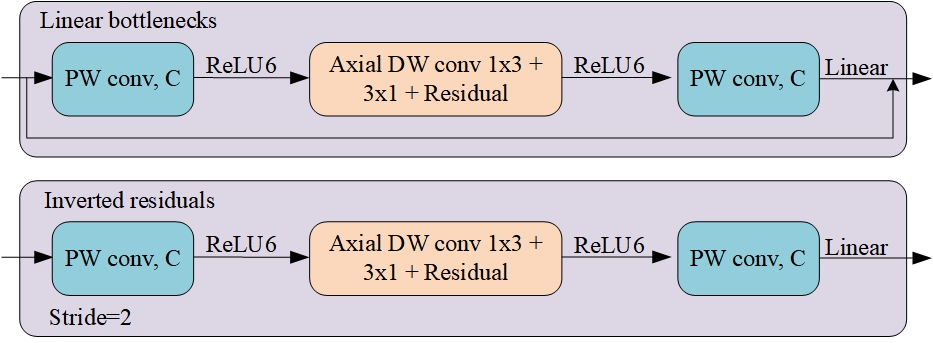
\includegraphics[width=0.7\linewidth]{picture/LLIE/My Architecture/Base module}
		%				%\captionsetup{font=scriptsize}
		%				\caption{Linear bottlenecks 和 Inverted residuals}
		%				\label{fig: Base module}	
		%		\end{figure}
	
	\subsection*{实验部分}
	
	如图\ref{fig: myplot_different_color_channels_low00010},图\ref{fig: myplot_different_color_channels_low00747},图\ref{fig: myplot_different_color_channels_low00776}所示, 我们观察到在 Y/Cb/Cr 色彩空间中,Y 通道并不总是能有效地表现出足够的亮度信息。相对而言,在 H/S/V 色彩空间中,H 和 S 通道似乎能通过色相和色彩饱和度的改变从而揭示出一定的图像纹理和结构信息,特别是在光照极低的情境下。这一发现指示了在处理低照度图像时,选择合适的色彩空间对于保留关键视觉信息至关重要。
	
	\begin{figure}[htbp]
		\centering
		\begin{subfigure}{0.3\textwidth}
			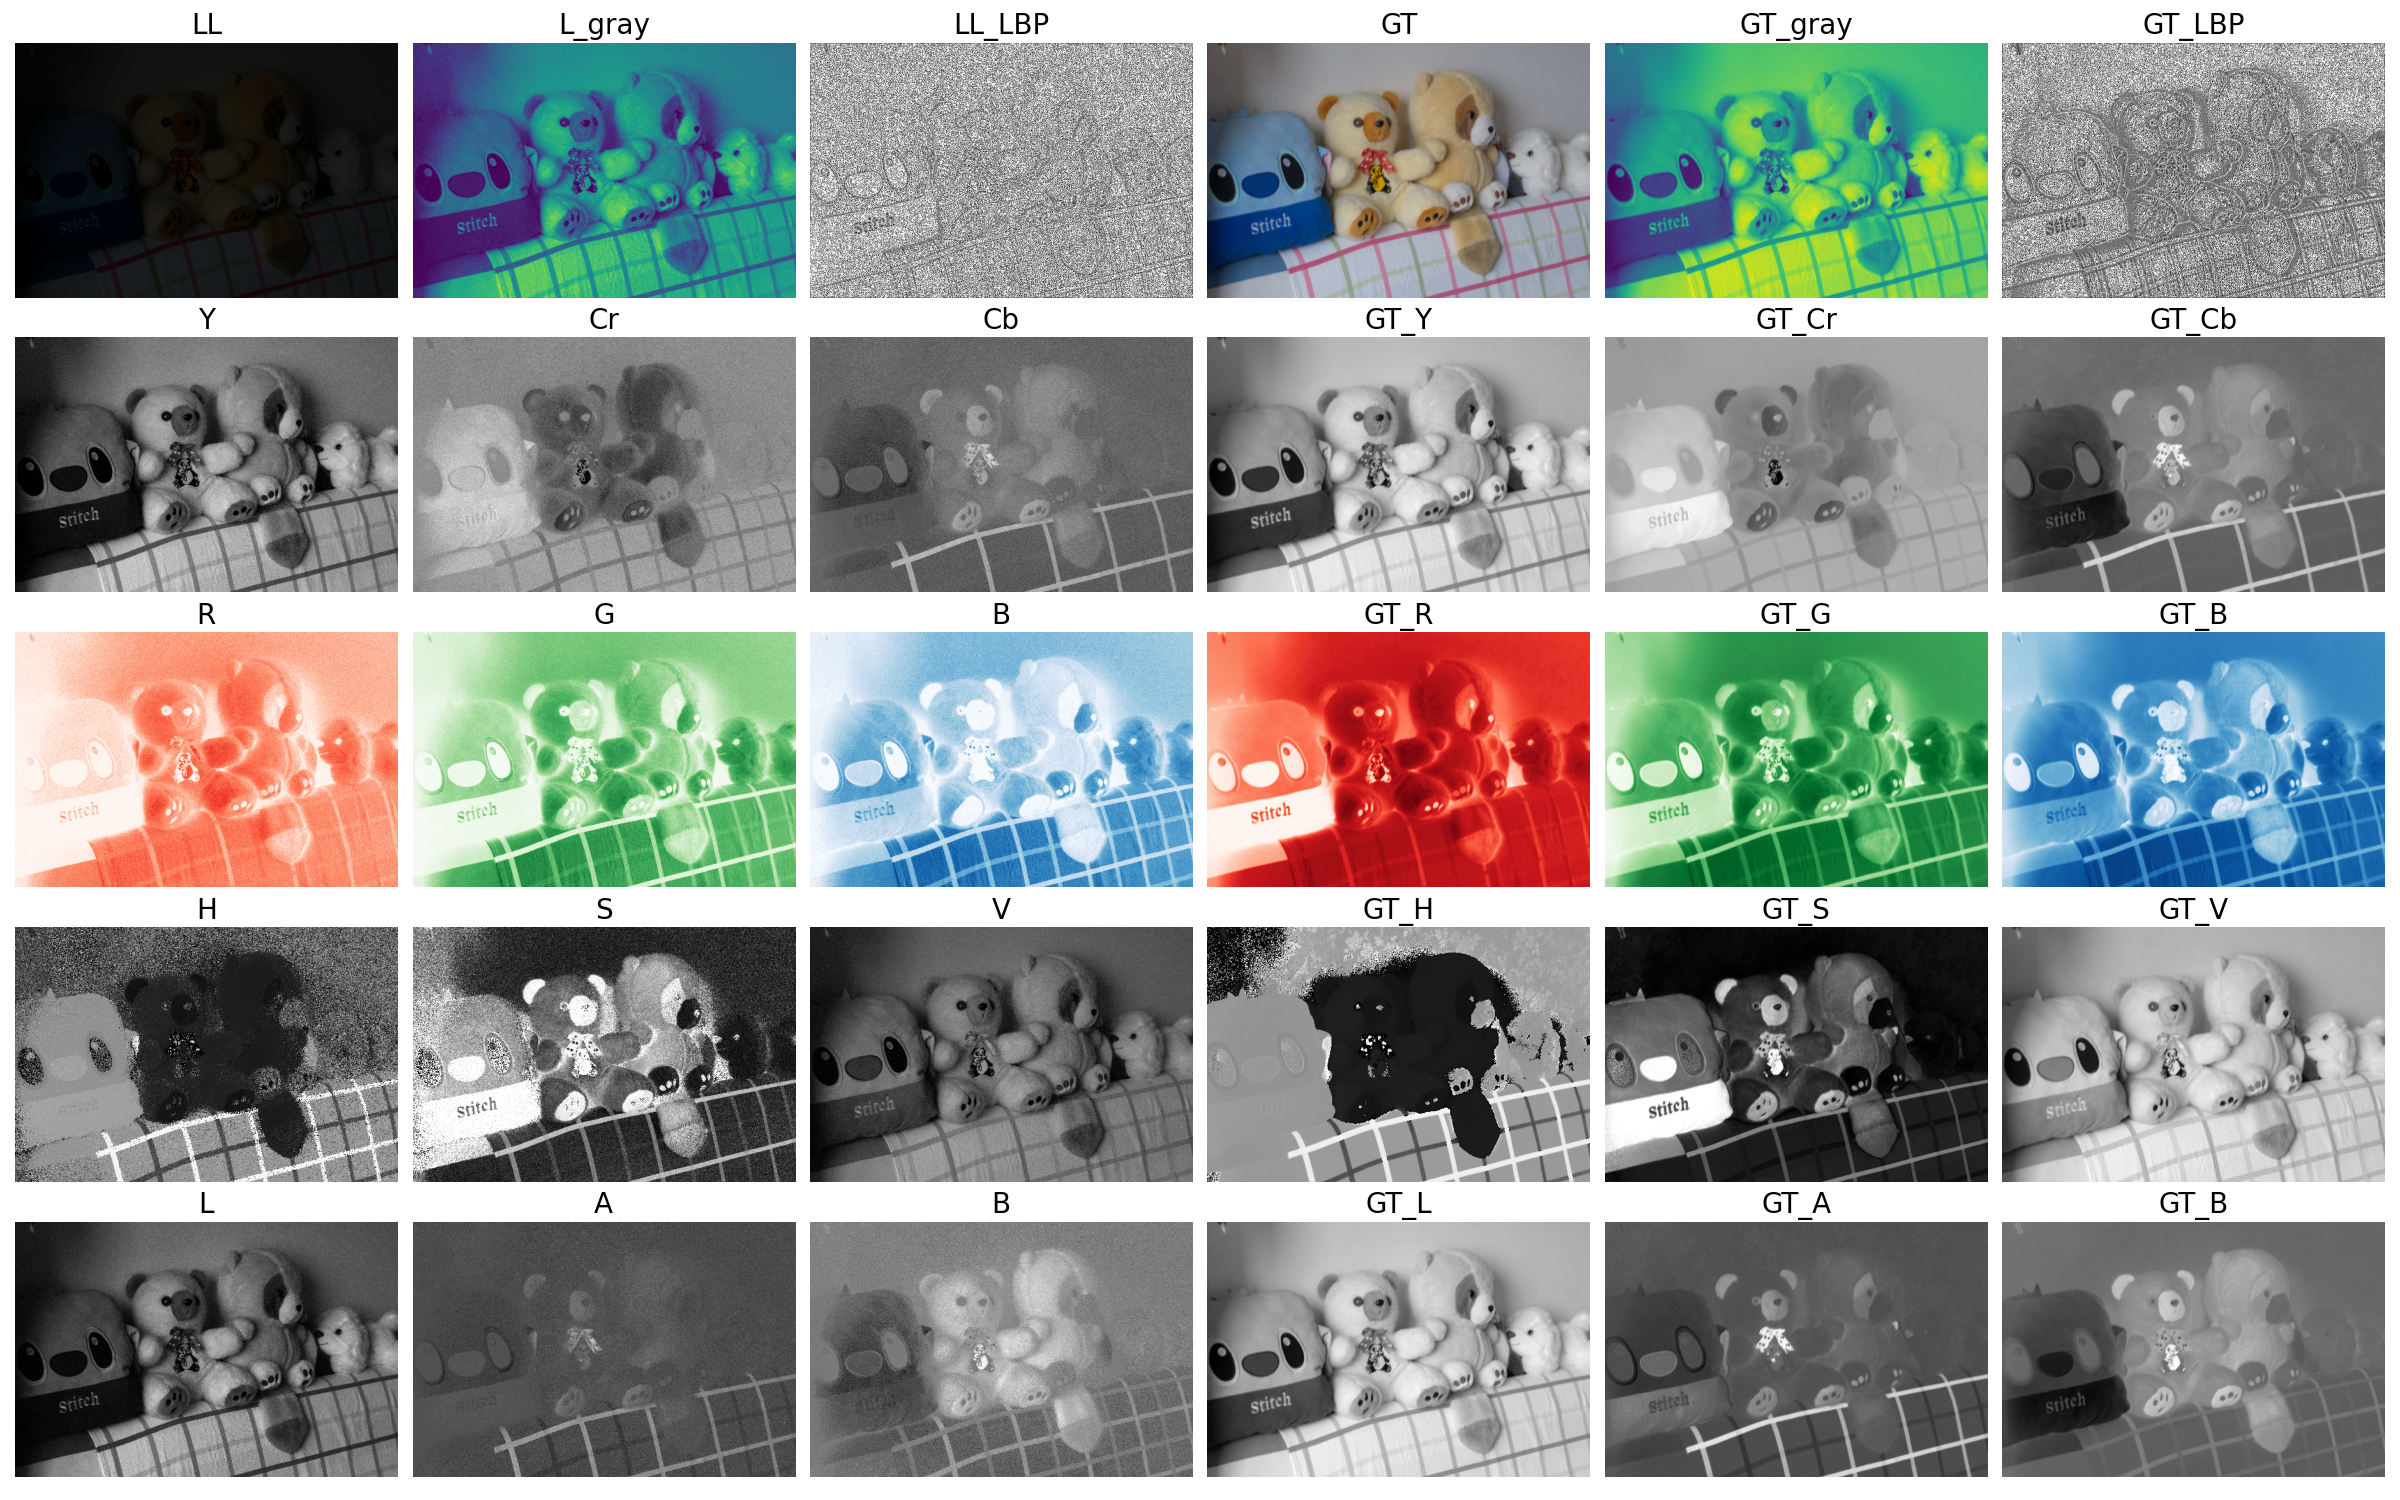
\includegraphics[width=\linewidth]{picture/LLIE/Experiment/myplot_different_color_channels_low00010}
			\captionsetup{font=scriptsize}
			\caption{low00010}
			\label{fig: myplot_different_color_channels_low00010}	
		\end{subfigure}
		\begin{subfigure}{0.3\textwidth}
			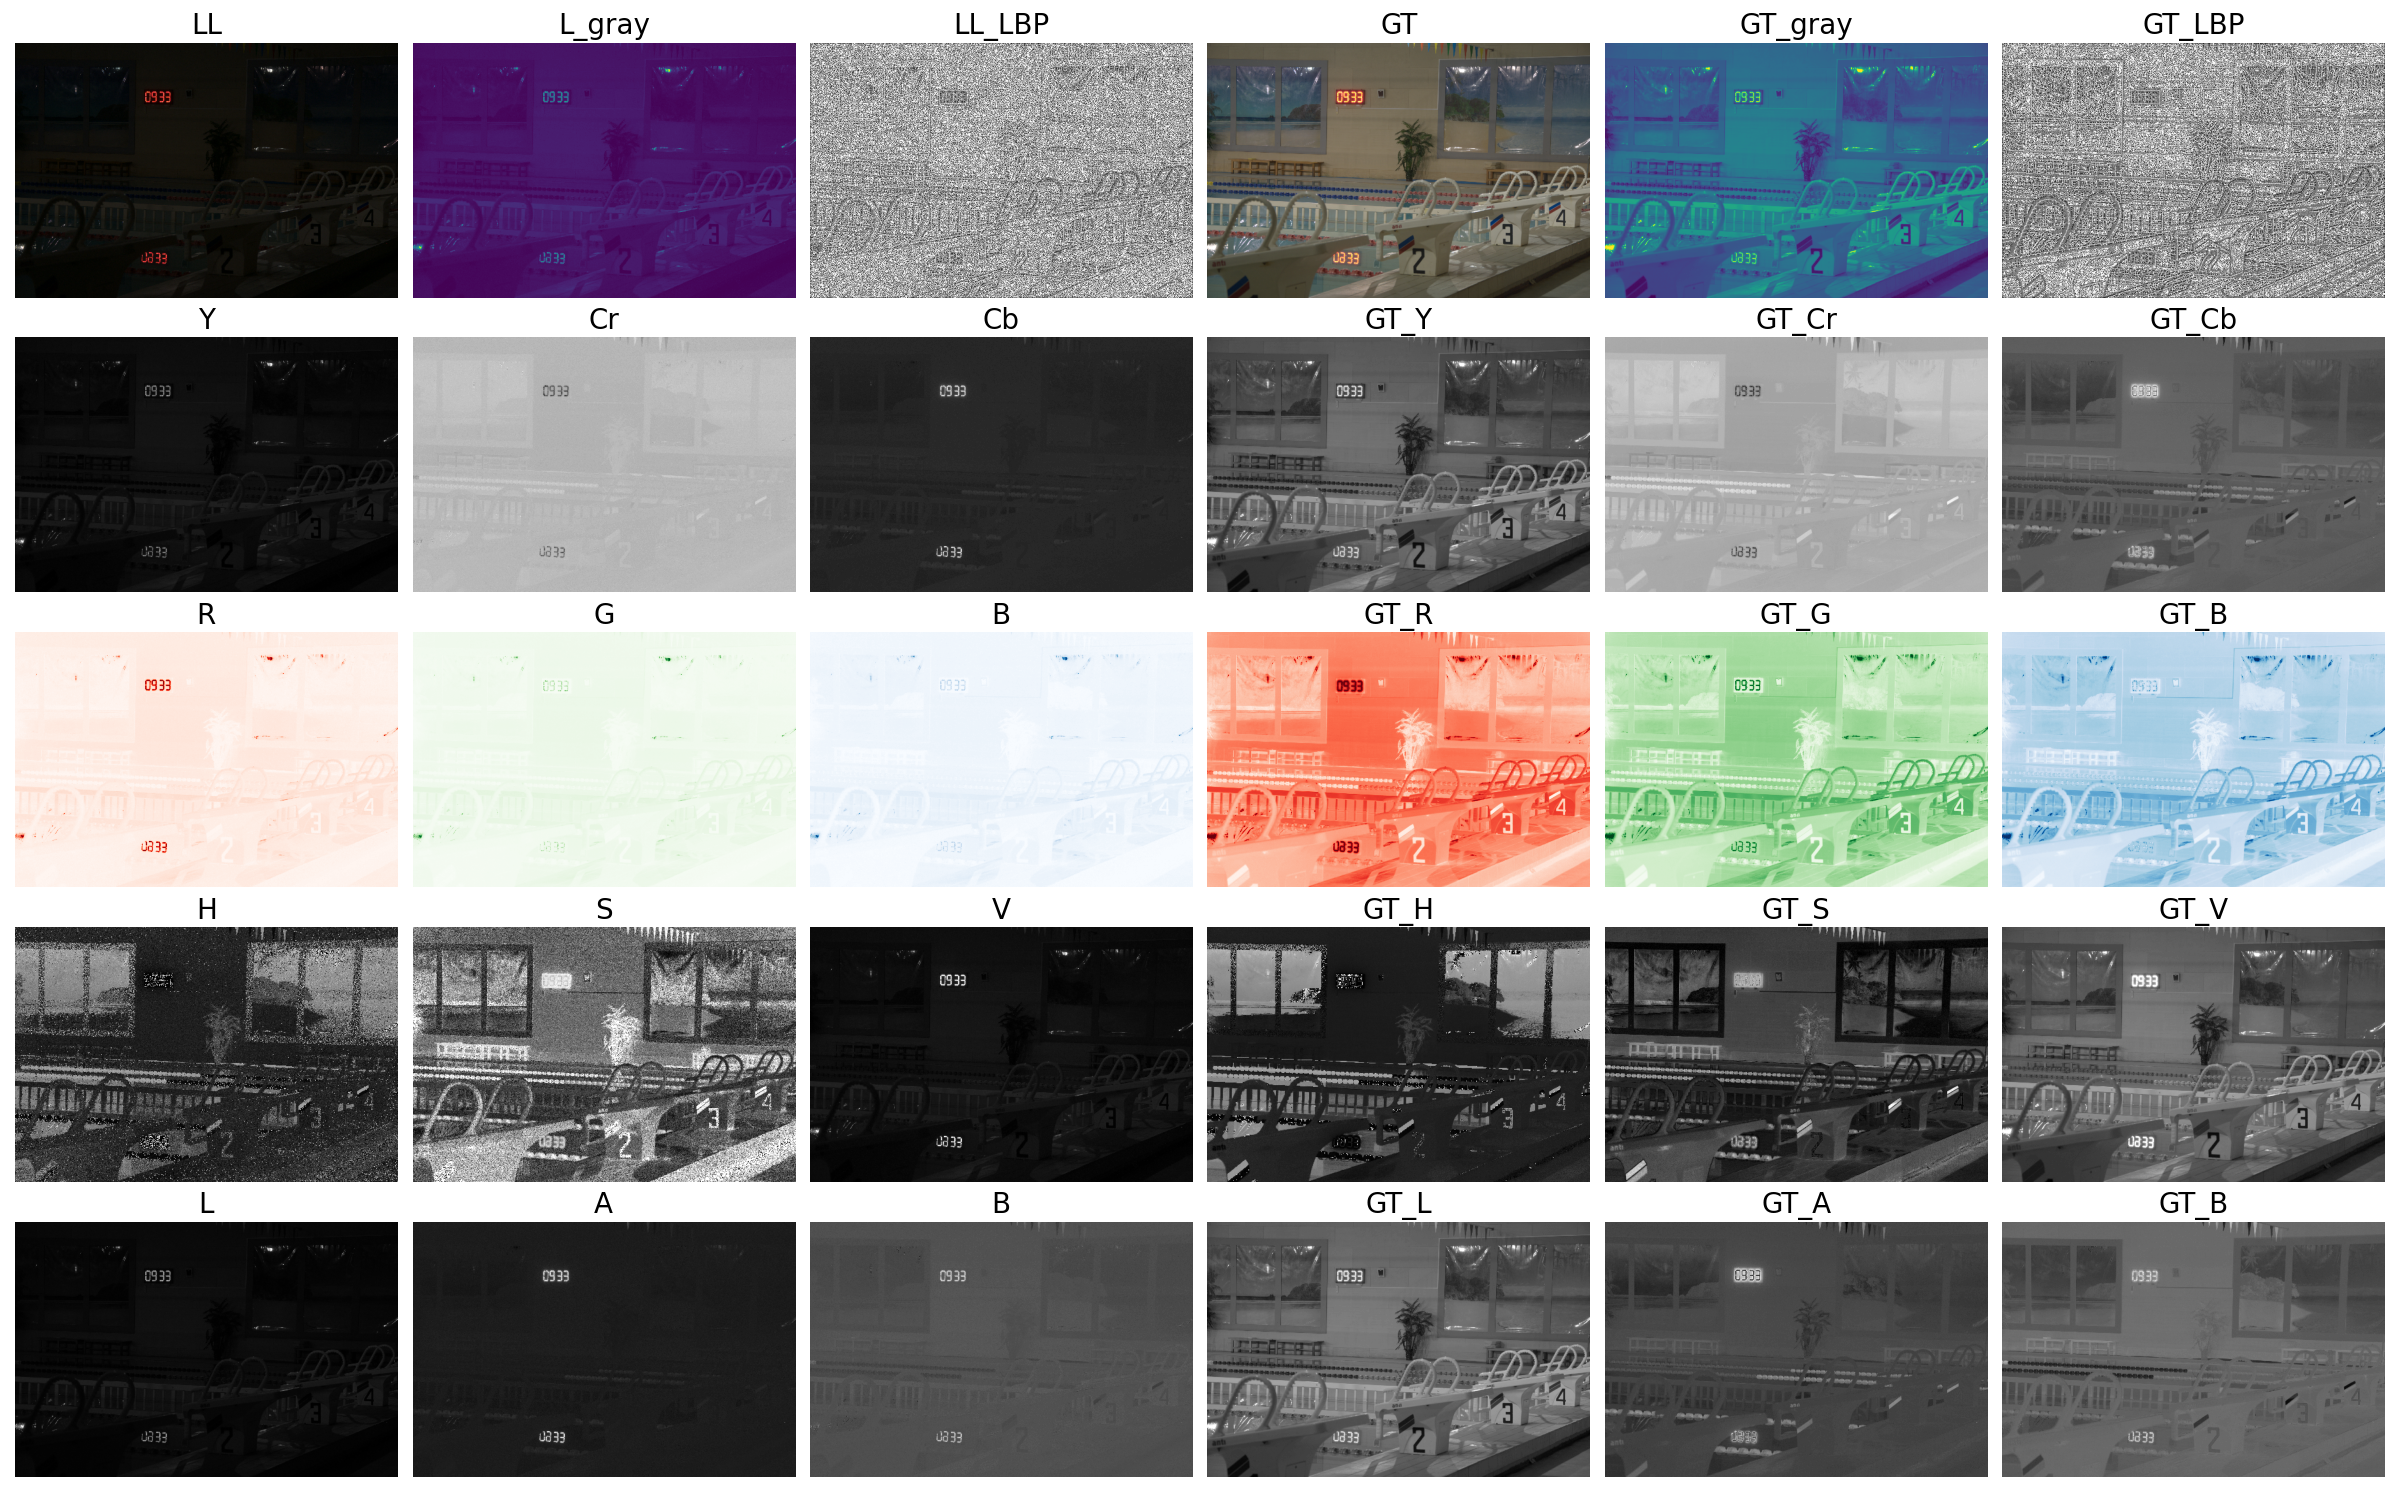
\includegraphics[width=\linewidth]{picture/LLIE/Experiment/myplot_different_color_channels_low00747}
			\captionsetup{font=scriptsize}
			\caption{low00747}
			\label{fig: myplot_different_color_channels_low00747}	
		\end{subfigure}
		\begin{subfigure}{0.3\textwidth}
			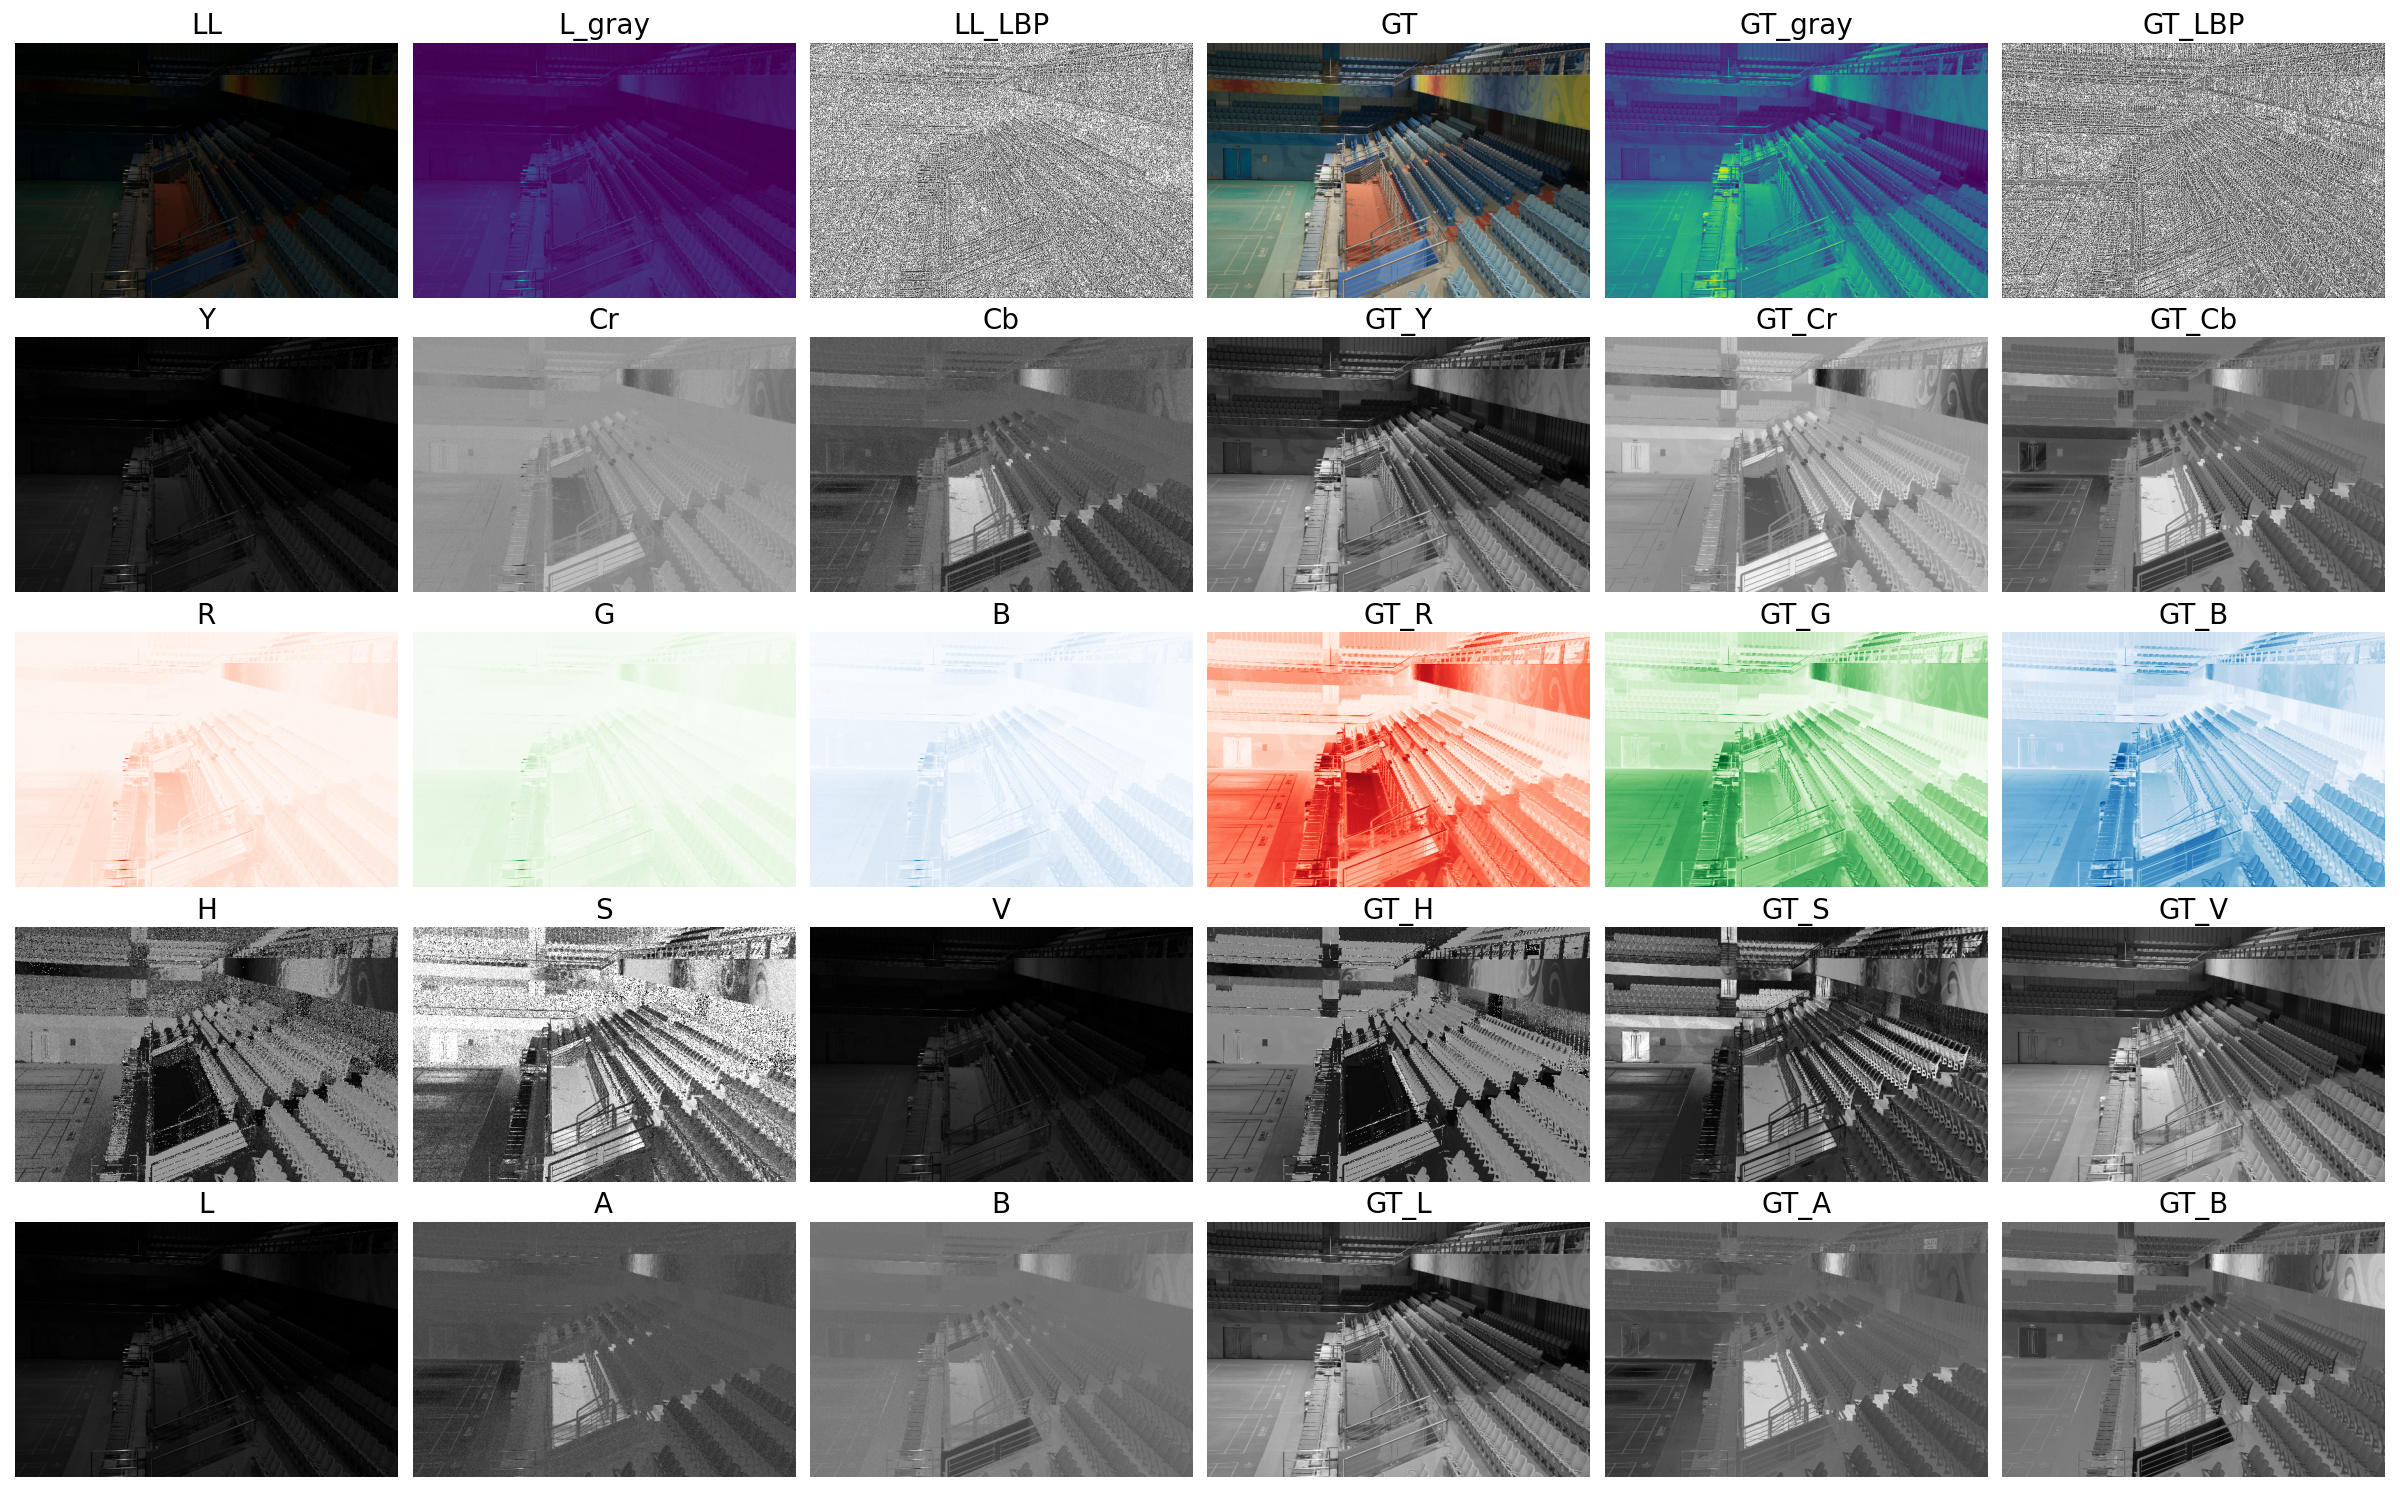
\includegraphics[width=\linewidth]{picture/LLIE/Experiment/myplot_different_color_channels_low00776}
			\captionsetup{font=scriptsize}
			\caption{low00776}
			\label{fig: myplot_different_color_channels_low00776}	
		\end{subfigure}\\
		\begin{subfigure}{0.3\textwidth}
			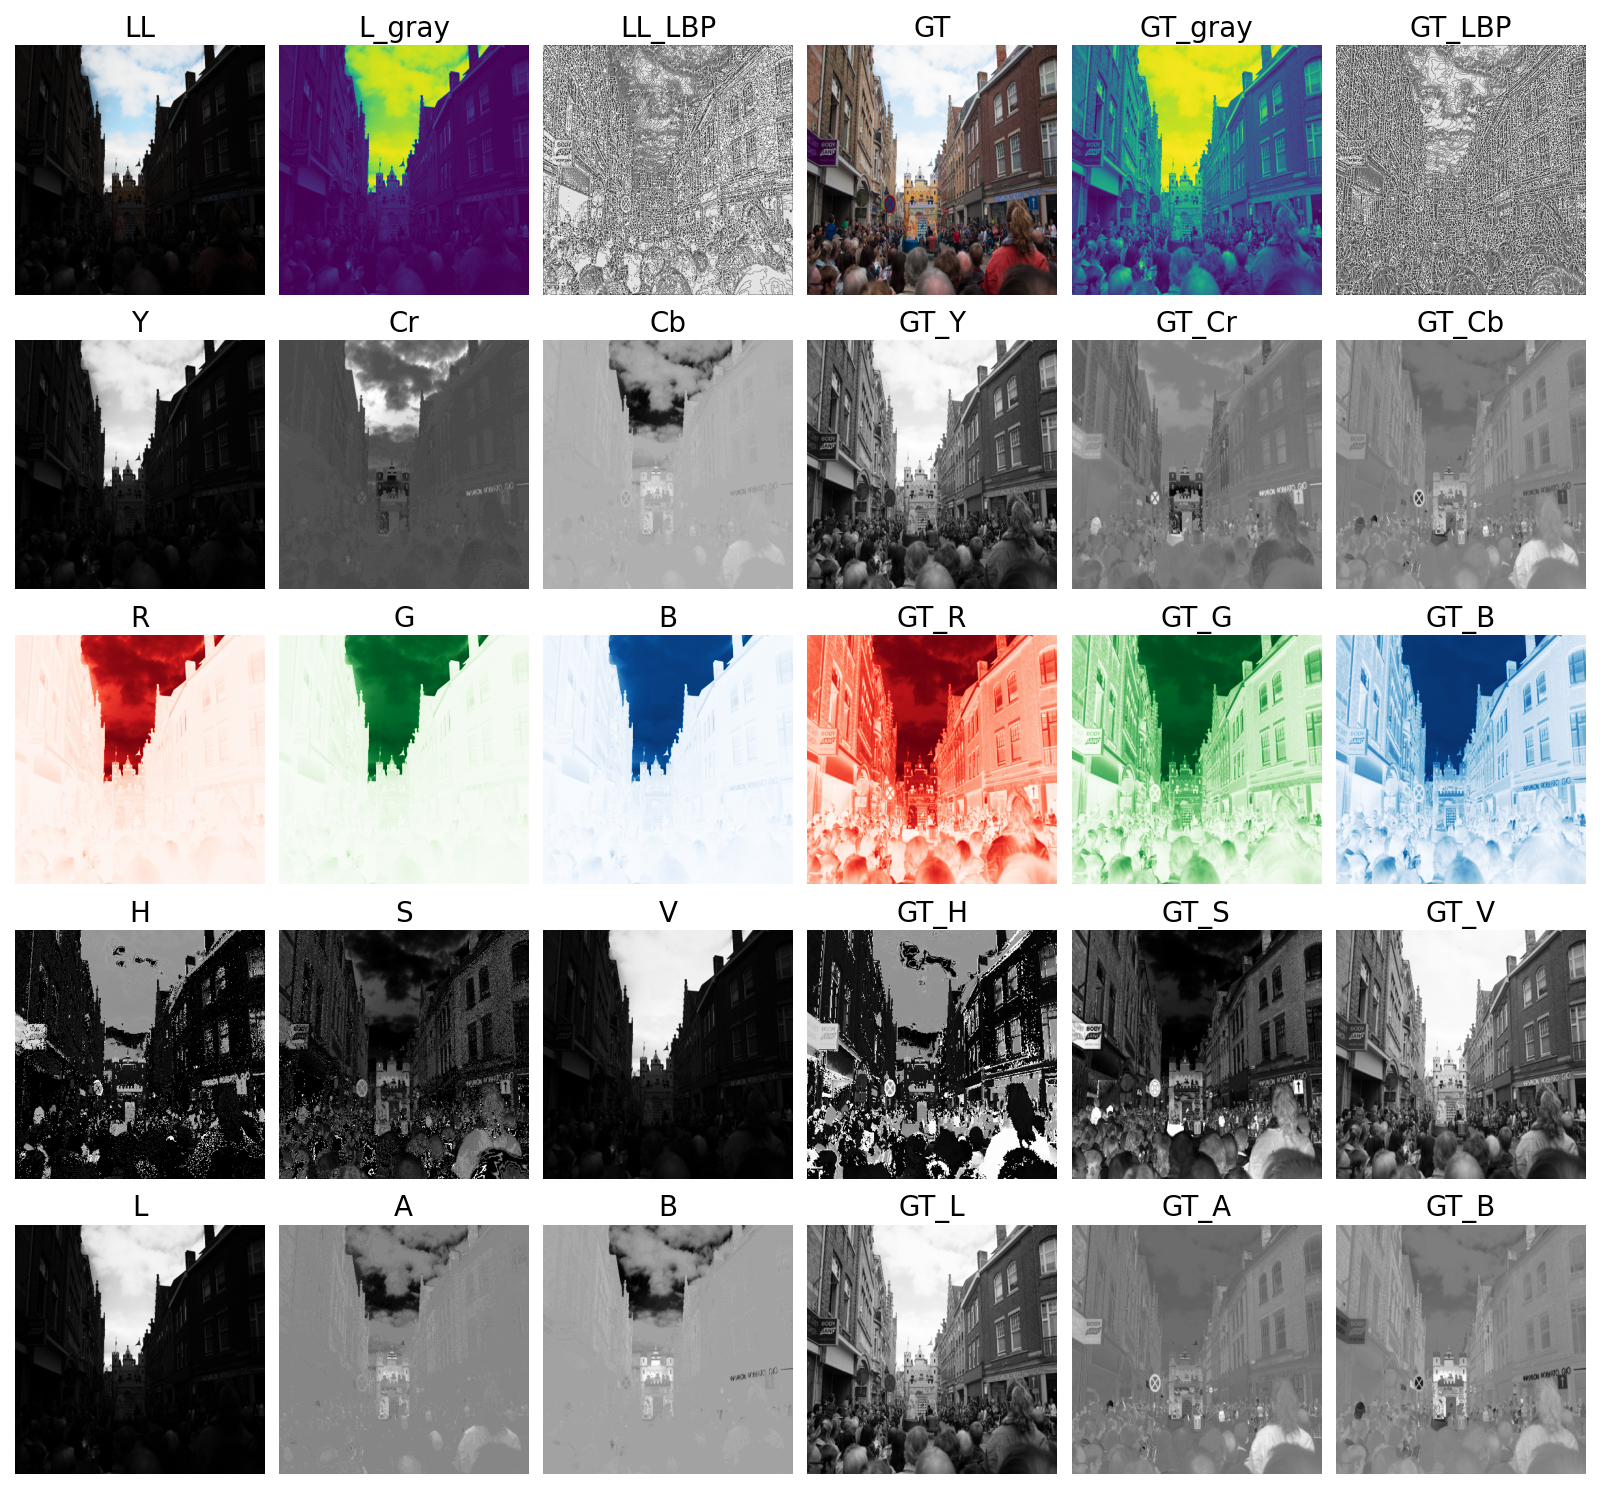
\includegraphics[width=\linewidth]{picture/LLIE/Experiment/myplot_different_color_channels_r097088c1t}
			\captionsetup{font=scriptsize}
			\caption{r097088c1t}
			\label{fig: myplot_different_color_channels_r097088c1t}	
		\end{subfigure}
		\begin{subfigure}{0.3\textwidth}
			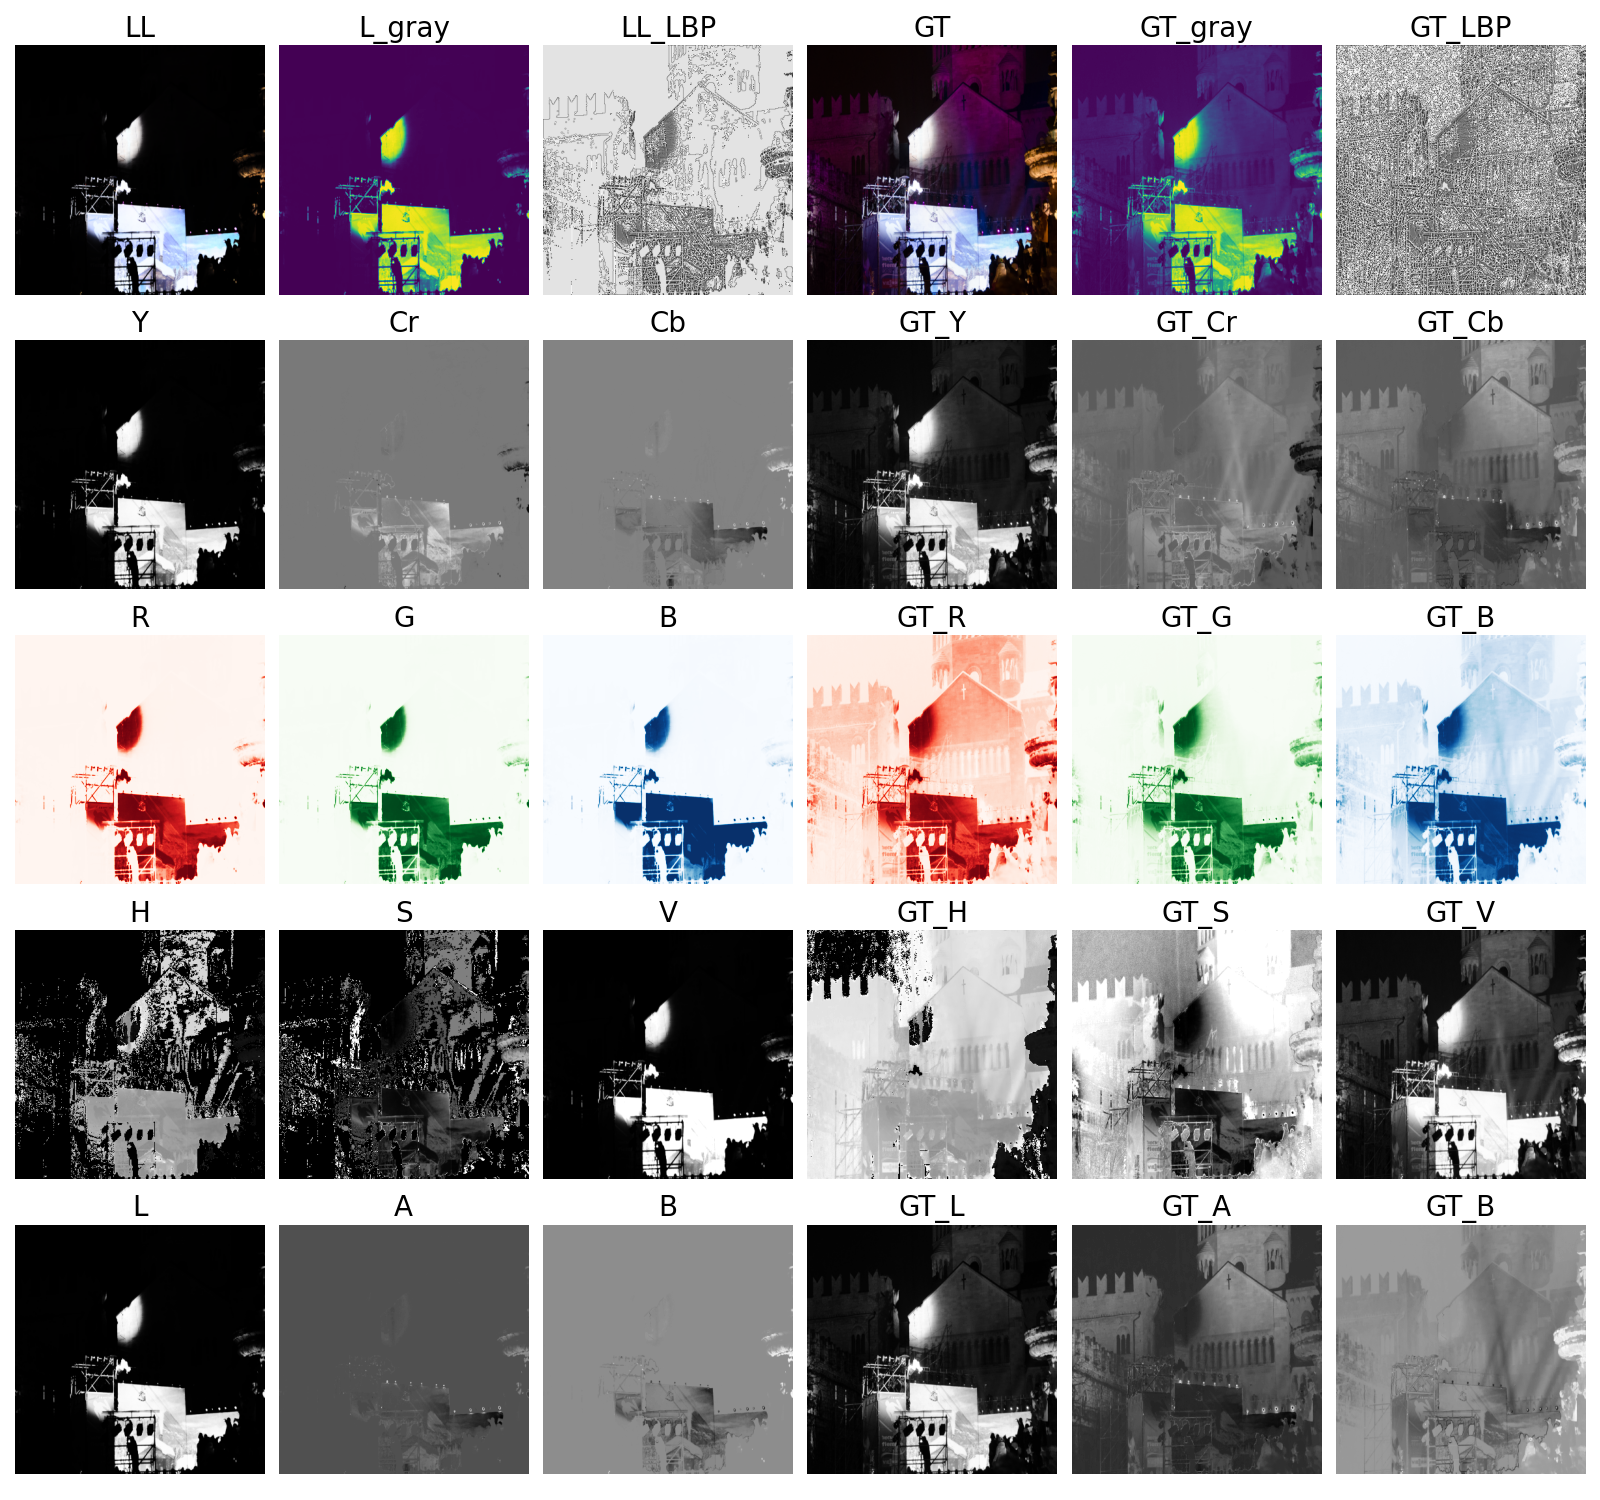
\includegraphics[width=\linewidth]{picture/LLIE/Experiment/myplot_different_color_channels_r141669e5t}
			\captionsetup{font=scriptsize}
			\caption{r141669e5t}
			\label{fig: myplot_different_color_channels_r141669e5t}	
		\end{subfigure}
		\begin{subfigure}{0.3\textwidth}
			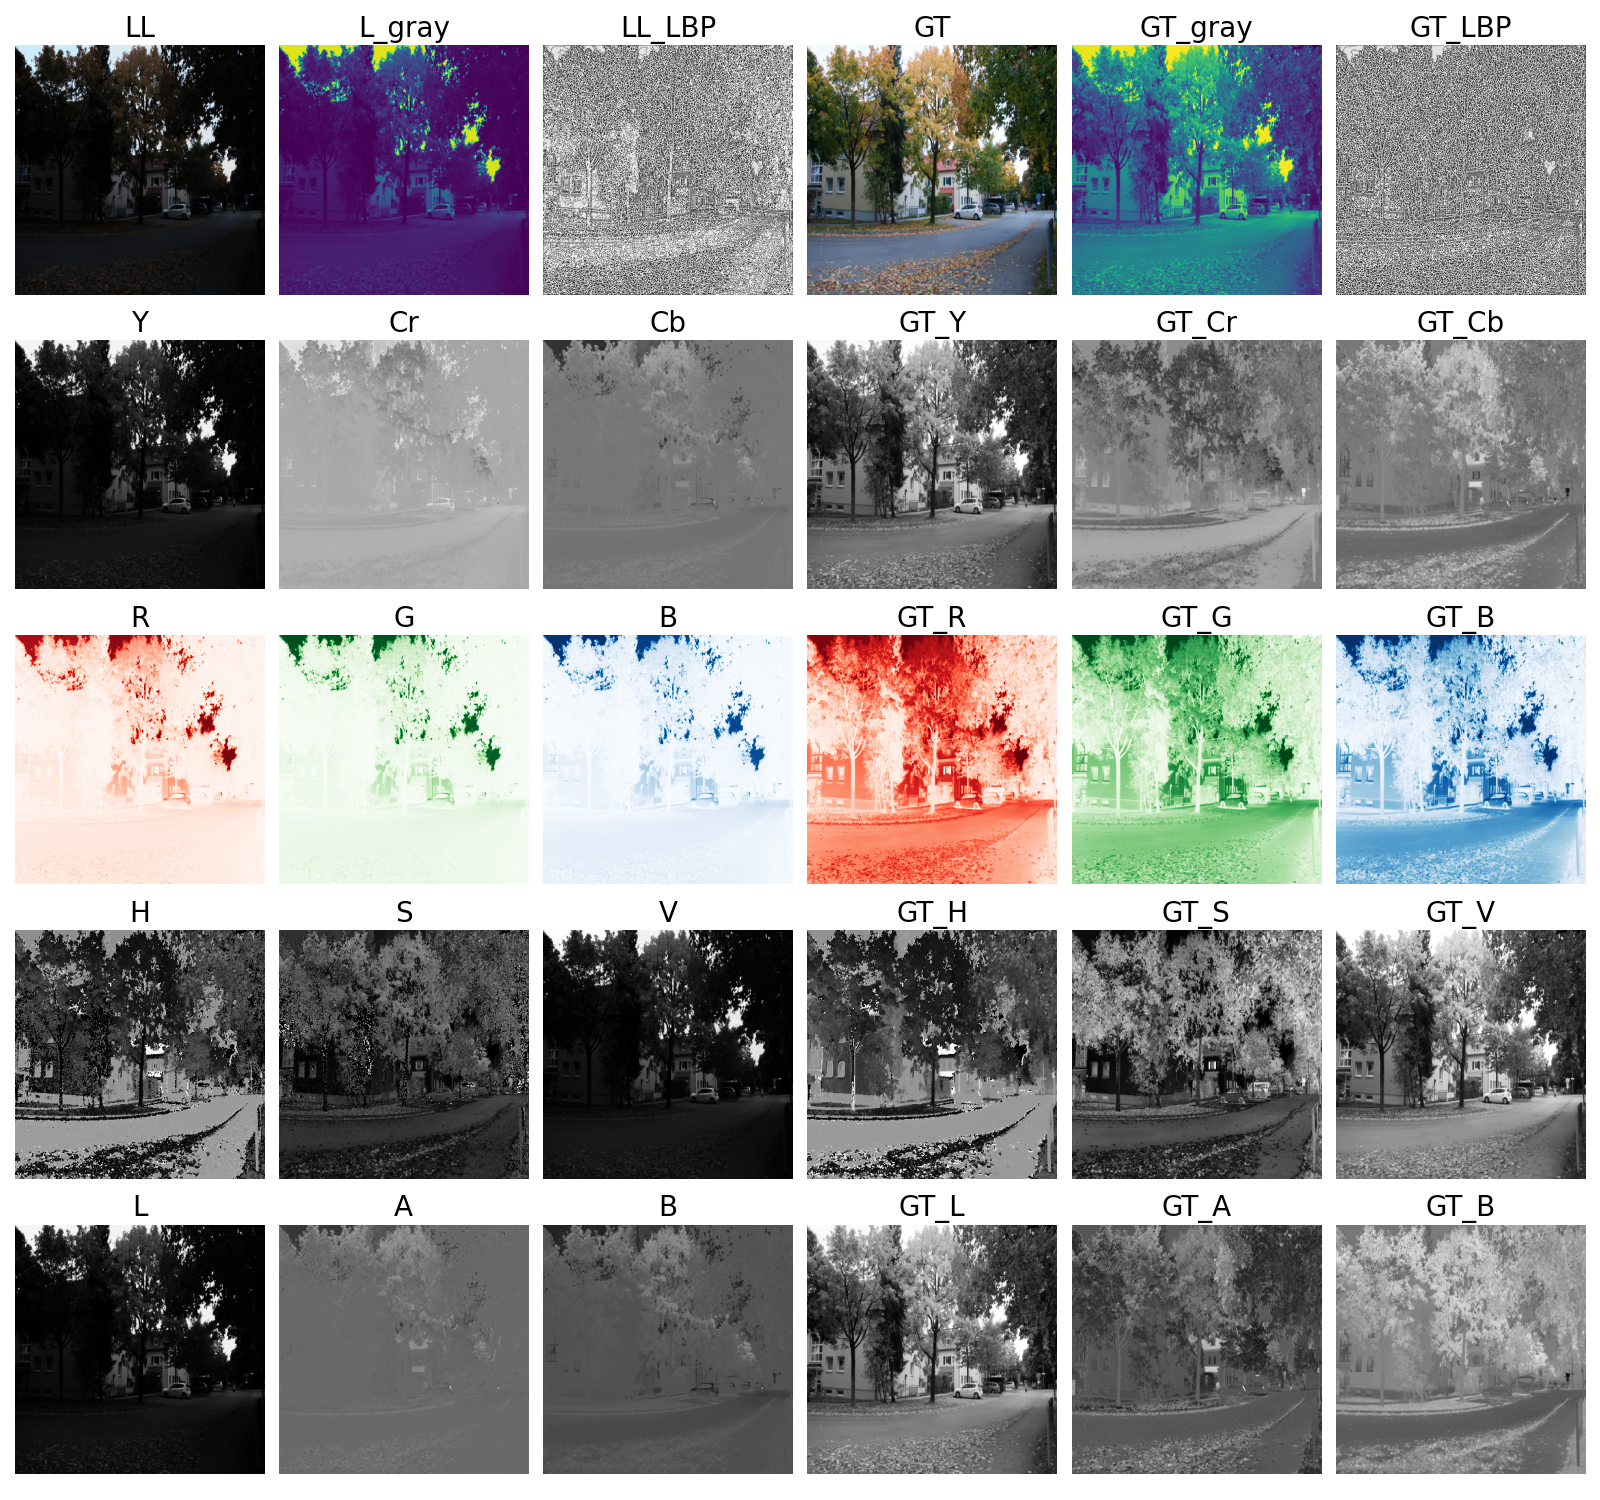
\includegraphics[width=\linewidth]{picture/LLIE/Experiment/myplot_different_color_channels_r145221d9t}
			\captionsetup{font=scriptsize}
			\caption{r145221d9t}
			\label{fig: myplot_different_color_channels_r145221d9t}	
		\end{subfigure}
		\caption{LOL-v2数据集中不同图片在 Y/Cb/Cr,HSV,LAB,RGB通道下的分离。 }
	\end{figure}
	
	\FloatBarrier
	
	在图\ref{fig: myplot_different_color_channels_low00010}中展示的 low00010 图像分析中,我们可以观察到低光条件下的RGB通道图片已经相对清晰。对应的 GT 图片主要显示了颜色的加深。此外,通过比较低光图像与 GT 图像的 Y 通道,我们可以发现亮度特征得到了良好的体现。然而,在 low00747 和 low00776 图像中,如图\ref{fig: myplot_different_color_channels_low00747}和图\ref{fig: myplot_different_color_channels_low00776}所示,相比于 low00010 图像,这两张图片的RGB通道所提供的信息明显不足以支持有效的图像增强。在这些图像中,Y/Cb/Cr通道的 Y 通道同样未能提供足够的信息以供增强处理。
	
	在人造低光图像的情况中,这种信息缺失更为明显,如图\ref{fig: myplot_different_color_channels_r097088c1t}、图\ref{fig: myplot_different_color_channels_r141669e5t}和图\ref{fig: myplot_different_color_channels_r145221d9t}所示。这些结果表明,在处理不同的图像数据时,简单的颜色加深或亮度增强可能不足以恢复图像质量,特别是当原始数据在关键通道中缺乏足够信息时。
	
	
	在对 HSV 色彩空间进行研究时,我们特别关注了 H(Hue) 通道(色调)的特性。色调通道的分析表明,它能够有效地揭示图像中的颜色种类。在低光环境下拍摄的图像中,H 通道不仅保留了颜色信息,而且清晰地展示了颜色的变化,这些变化在此环境下可视作“颜色噪声”。通过细致分析H通道,我们可以更有效地把握图像的纹理特征,并恢复出更接近真实场景的颜色表现。我们似乎通过综合利用色调通道提供的独特颜色识别能力,可以在不同光照条件下实现更精确的颜色复原,从而为低光图像处理提供了一种新的视角和方法论。
	
	S (Saturation)通道表示颜色的纯度或浓度,即色彩的深浅程度。饱和度为 0 表示灰度图像,而饱和度为 1 表示完全饱和的纯色。在某些情况下,饱和度图像可能反映出图片的一些结构信息。饱和度一般反映了像素的颜色纯度或浓度,较高的饱和度意味着颜色更加纯净和饱和,而较低的饱和度则意味着颜色更加灰暗和淡薄。在一些图像中,物体的边界或者纹理部分可能具有较高的饱和度,而背景或者平坦的区域可能具有较低的饱和度。因此,在一些情况下,饱和度图像可能会显示出物体的边界或者纹理信息。但是,并不是所有的图像都能够通过饱和度图像准确地反映出结构信息。在某些情况下,饱和度图像可能会受到光照,色彩分布和摄像机参数等因素的影响,导致其无法准确地反映出图像地结构信息。对于低光图像来说,饱和度(S)通道通常不能很好地反映出图片地结构信息。低光图像通常是指光照条件较差或者光照不均匀的图像,在这种情况下,图像的色彩信息可能会受到影响,导致饱和度较低,即使存在一定的色彩变化或者结构信息,也可能无法很好地体现在饱和度通道中。
	
	V (Value)通道表示颜色的亮度或明暗程度。明度为 0 表示黑色,而明度为 1 表示白色。对于低光图像来说,亮度(V)通道通常能够更好地反映出图片的结构和纹理信息。亮度通道代表了图像的明暗程度,而在低光条件下,图像的色彩信息可能会受到影响,导致饱和度和色调较低,即使存在一定的色彩变化或者结构信息,也可能无法很好地体现在饱和度和色调通道中。综上所述,对于低光图像更适合使用亮度(V)通道来反映图片的结构信息。
	
	\subsection*{采用方法和策略}
	
	我们采用的方法如图\ref{fig: HSV Architecture}所示。
	
	\begin{figure}[htbp]
		\centering
		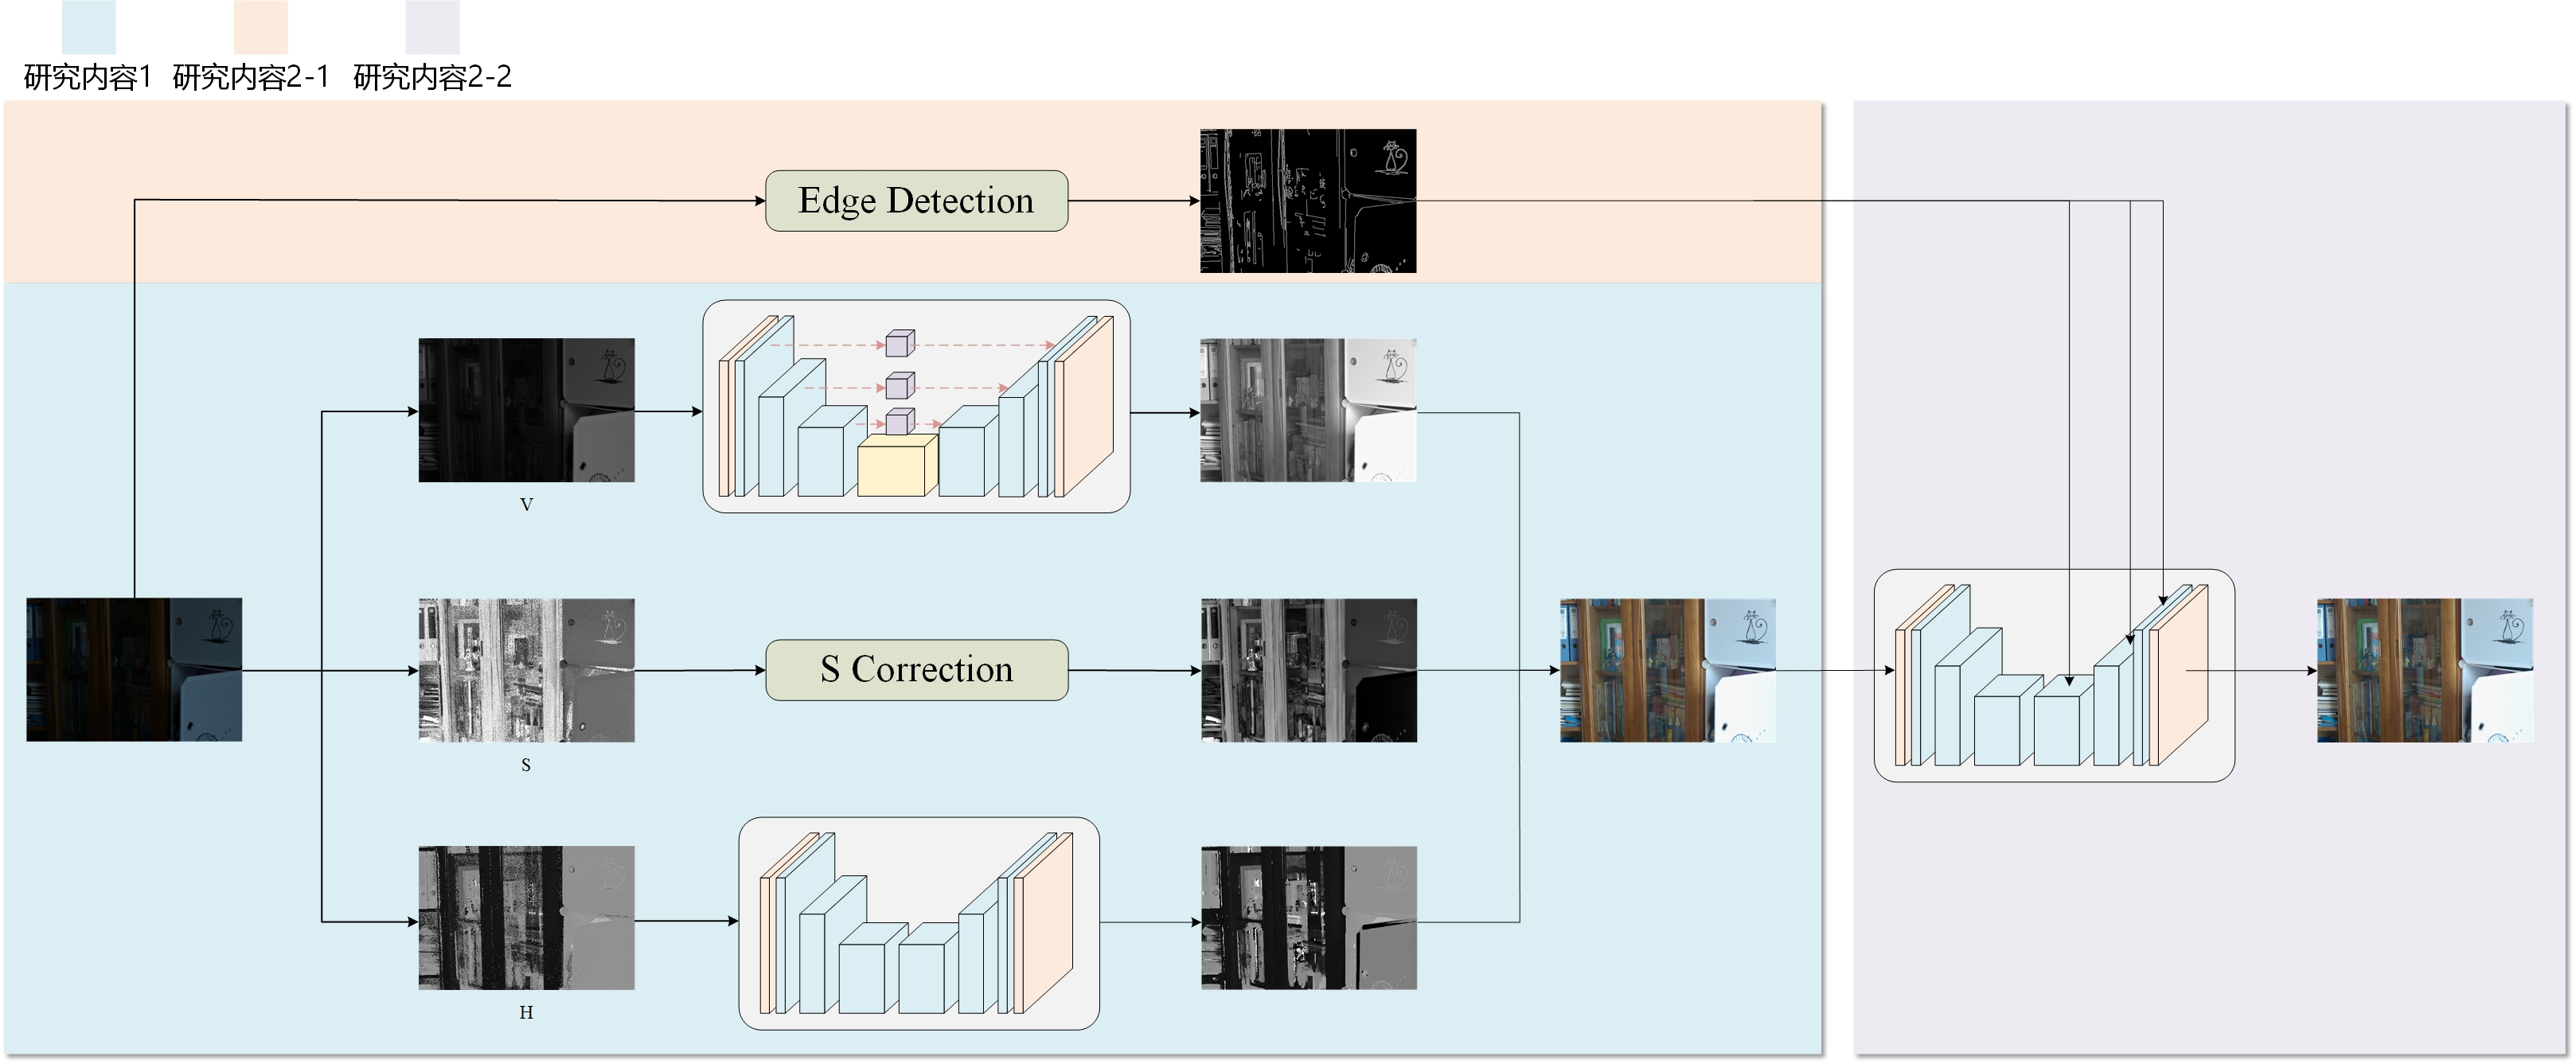
\includegraphics[width=0.7\linewidth]{picture/LLIE/My Architecture/HSV Architecture}
		%\captionsetup{font=scriptsize}
		\caption{整体模型架构}
		\label{fig: HSV Architecture}	
	\end{figure}
	
	在 V 通道中,我们致力于还原图像的边缘,纹理细节,并通过特定的设计,使得模型在对低光区域内的边缘和纹理也有较高的增强能力。此外,V 通道需要具备一定的去噪能力,抑制噪声的增强。在 S 通道中,我们致力于校正 S 通道,使其匹配我们所增强的 V 通道。常见的饱和度增强的方法有线性拉伸,直方图均衡化等,但是这些方法在校正饱和度分量,往往会导致图像失真。我们采用如下校正饱和度分量进行增强的方法,如式\ref{eq: S channel Correction}。
	
	\begin{equation}
		\begin{aligned}
			S_{c} = S + t(V_{c} - V)\varepsilon
		\end{aligned}
		\label{eq: S channel Correction}
	\end{equation}
	
	其中$S_{c}$表示增强的 S 通道成分,$V_{c}$表示增强的 V 通道成分,$t$为常量,$\varepsilon$为调整系数,如式\ref{eq: an adjustment coefficient}。
	
	\begin{equation}
		\begin{aligned}
			\varepsilon (x, y) = \frac{\sum\limits_{i,j \in \Omega} \left(\left|V(i,j)-\bar{V}_{\Omega}(i,j)\right|\left|S(i,j)-\bar{S}_{\Omega}(i,j)\right|\right)}{\sqrt{\delta_{V}(x,y)\delta_{S}(x,y)}}
		\end{aligned}
		\label{eq: an adjustment coefficient}
	\end{equation}
	
	其中,$(x,y)$ 增强点位置,$\bar{V}_{\Omega}(i,j)$ 和 $\bar{S}_{\Omega}(i,j)$ 分别表示以增强点为中心 $N \times N$ 领域内所有点的平均高度值和饱和度值。$\delta_{V}(x,y)$和$\delta_{S}(x,y)$分别表示增强点的亮度方差和饱和度方差。$(i,j)$表示领域内像素的坐标。
	
	
	\FloatBarrier
	
	\subsection*{对注意力机制的创新改进方法}
	
	\subsubsection*{MSAM}
	
	我们将多尺度卷积注意模块 (Multi-scale convolutional attention, MSCA) 引入 CBAM 模块中,使得通道注意力也具备多尺度性能,多分支深度卷积或许可以更好的提取多尺度特征,如图\ref{fig: MSAM} 所示。
	
	\begin{figure}[htbp]
		\centering
		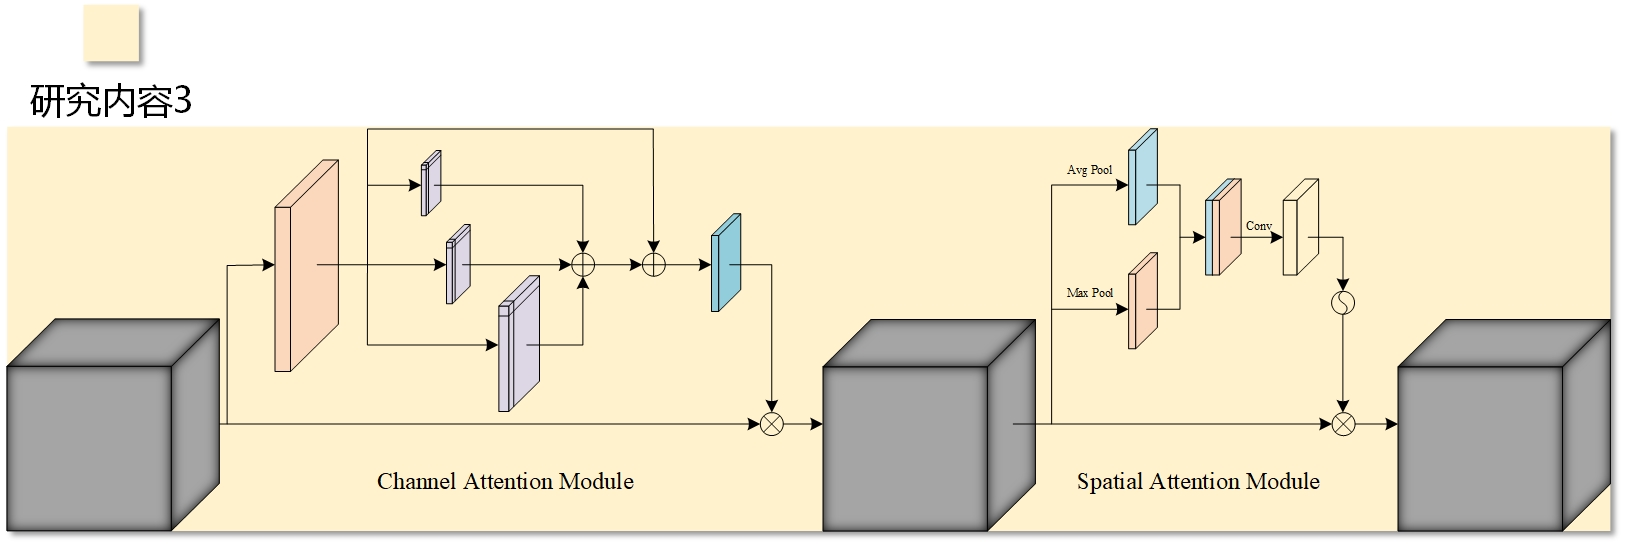
\includegraphics[width=0.8\linewidth]{picture/LLIE/Experiment/Attention/MSAM}
		%\captionsetup{font=scriptsize}
		\caption{MSAM}
		\label{fig: MSAM}
	\end{figure}
	
	具体来说,MSCA 首先通过一个 $5 \times 5$ 的卷积核进行卷积操作,然后分别使用 $7 \times 7$、$11 \times 11$ 和 $21 \times 21$ 的多尺度深度卷积核对特征图进行处理,以捕捉不同尺度的特征信息。接着将这些尺度上的特征图相加,并与输入的残差特征相加,最后通过一个 $1 \times 1$ 的卷积核对通道进行调整,以获得最终的注意力特征表示。
	
	\subsubsection*{CPCS}
	
	%		SegNeXt 是一种用于语义分割的简单卷积网络体系结构\cite{guo2022segnext},作者通过对已有成功分割方案进行了重新审视,发现了几个有助于性能提升地关键成分,进而促使作者设计了一种新型地卷积注意力架构方案,多尺度卷积注意模块(Multi-scale convolutional attention, MSCA),其原理主要是将 CBAM 块中的通道注意力替换为 MSCA,使通道注意力具备多尺度性能。MSCA块证明了卷积注意比Transformer中的自注意机制更有效地编码上下文信息。
	%		
	%		如图\ref{fig: MSCA} 所示,MSCA包含三个部分:深度卷积聚合局部信息,多分支深度可分离卷积捕获多尺度上下文,以及 $1 \times 1$ 卷积建模不同通道之间的关系。通过采用多尺度深度卷积模块,可以有效地提取空间关系,同时保留通道先验\cite{huang2023channel}。
	%		
	%		\begin{figure}[htbp]
		%			\centering
		%			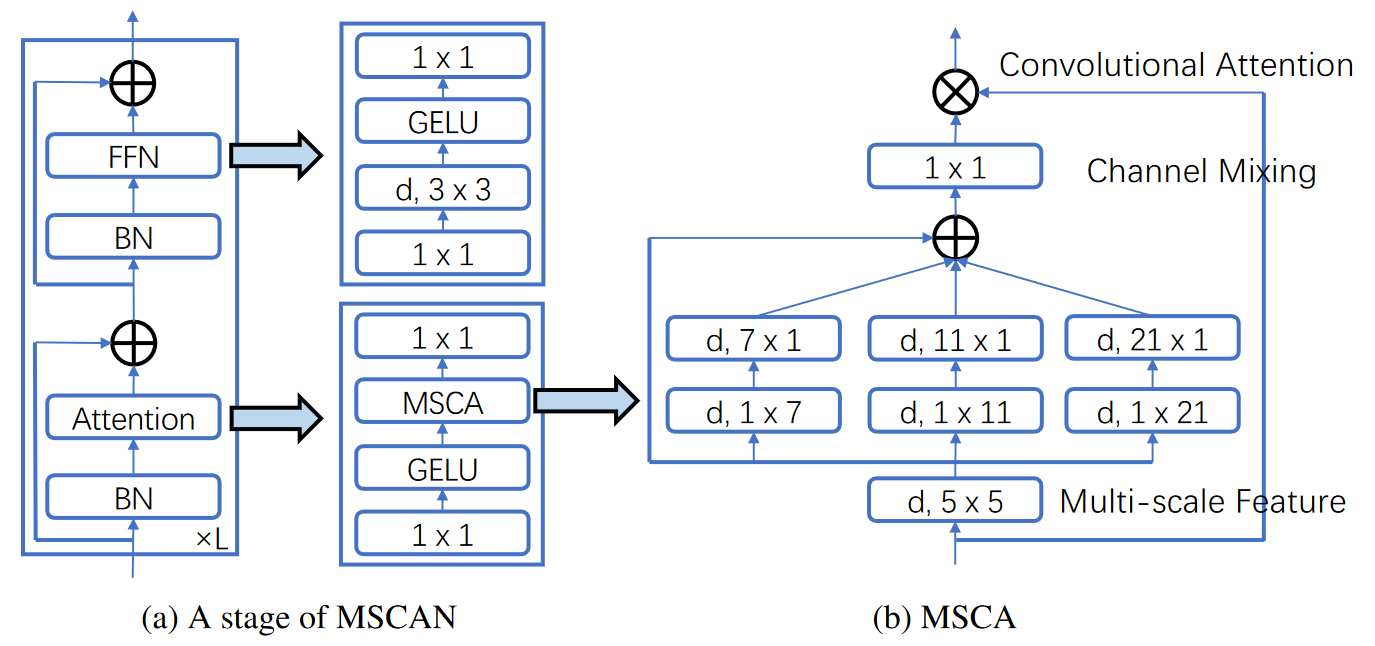
\includegraphics[width=0.8\linewidth]{picture/LLIE/Experiment/Attention/MSCA}
		%			%\captionsetup{font=scriptsize}
		%			\caption{MSCA}
		%			\label{fig: MSCA}
		%		\end{figure}
	%			
	%	 	SE 只整合了通道注意力,这限制了它选择重要区域的能力。
	
	CBAM 整合了通道注意力和空间注意力,但它在其输出特征的所有通道上强制执行一致的空间注意力分布。如图\ref{fig: SE_CBAM_CPCA}(c)所示,作者\cite{huang2023channel}提出一种新的通道优先卷积注意力(Channel Prior Convolutional Attention, CPCA)方法,采用多尺度的深度可分离卷积模块构成空间注意力,可以在通道和空间维度上动态分配注意权重。
	
	\begin{figure}[htbp]
		\centering
		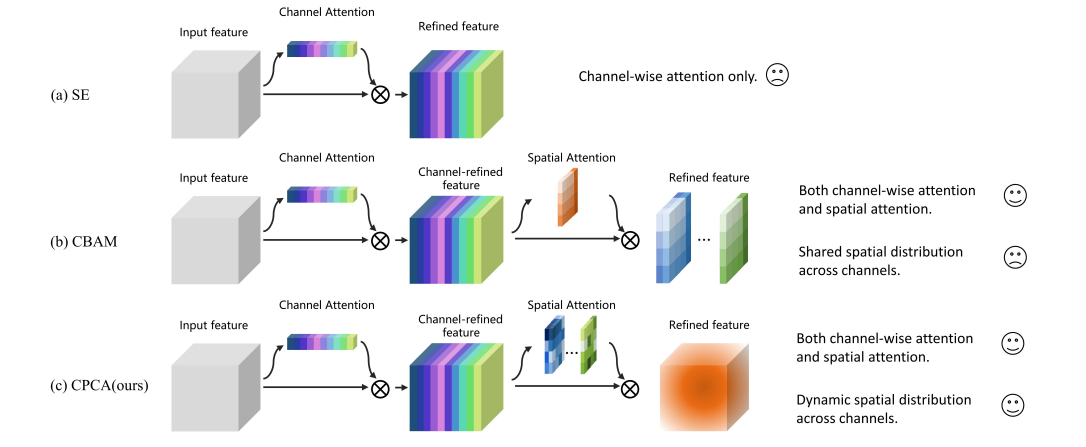
\includegraphics[width=0.8\linewidth]{picture/LLIE/Experiment/Attention/SE_CBAM_CPCA}
		%\captionsetup{font=scriptsize}
		\caption{Schematic representation of the refined features of the three attention mechanisms (a) SE, (b) CBAM, and (c) CPCA.}
		\label{fig: SE_CBAM_CPCA}
	\end{figure}
	
	CPCA的整体结构包括通道注意力和空间注意力的顺序放置。特征图的空间信息是由通道注意力通过平均池化和最大池化等操作来聚合的。随后,空间信息通过共享多层感知器(shared MLP)进行处理并添加以生成通道注意力图。通道先验是通过输入特征和通道注意力图的元素相乘获得的。随后,通道先验被输入到深度卷积模块中以生成空间注意力图。卷积模块接收空间注意力图以进行通道混合。最终,通过通道混合结果与通道先验的逐元素相乘,获得细化的特征作为输出。多尺度深度可分离卷积注意力原理图见图\ref{fig: CPCA}.
	
	\begin{figure}[htbp]
		\centering
		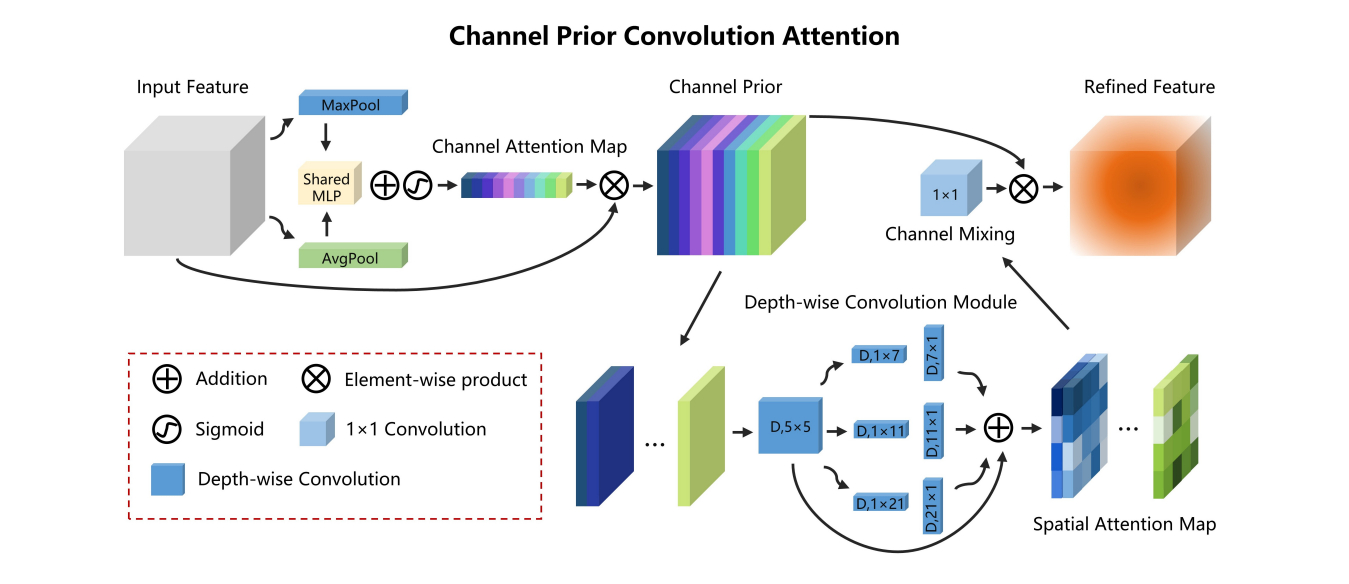
\includegraphics[width=0.8\linewidth]{picture/LLIE/Experiment/Attention/CPCA}
		%\captionsetup{font=scriptsize}
		\caption{CPCA}
		\label{fig: CPCA}
	\end{figure}
	
	我们结合上述两种方法,如图\ref{fig: CPMS} 所示,设计一种多尺度通道注意力和多尺度深度可分离卷积空间注意力(Channel Prior Multi-Scale Attention, CPMS)
	
	\begin{figure}[htbp]
		\centering
		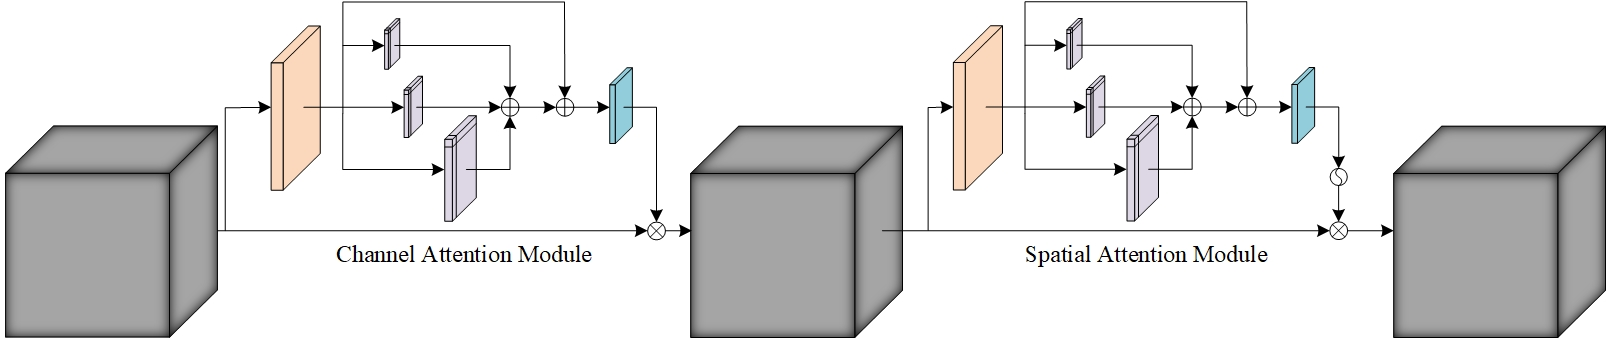
\includegraphics[width=0.8\linewidth]{picture/LLIE/Experiment/Attention/CPMS}
		%\captionsetup{font=scriptsize}
		\caption{CPMS}
		\label{fig: CPMS}
	\end{figure}
	
	
	\subsection*{对UNet网络的改进方法}
	
	我们尝试了不同的 Encoder 和 Decoder 组合,如图\ref{fig: Encoder and Decoder} 所示,对于 Encoder 部分,我们首先应用注意力机制(Attention),然后使用 $3 \times 3$ 的轴向深度可分离卷积 (Depthwise Separable Convolution),接着进行批标准化 (Batch Normalization) 和 $1 \times 1$ 卷积操作,最后通过最大池化 (MaxPooling) 进行特征压缩,最终使用 Sigmoid 激活函数。对于 Decoder 部分,我们首先将其与对应的 Encoder 的跳跃连接进行 Concat 操作,然后进行上采样 (Upsample) 操作,接着应用注意力机制 (Attention) ,再次使用 $3 \times 3$ 的轴向深度可分离卷积,再通过批标准化和 $1 \times 1$ 卷积操作,最终采用 PReLU 激活函数。
	
	\begin{figure}[htbp]
		\centering
		\begin{subfigure}{0.5\textwidth}
			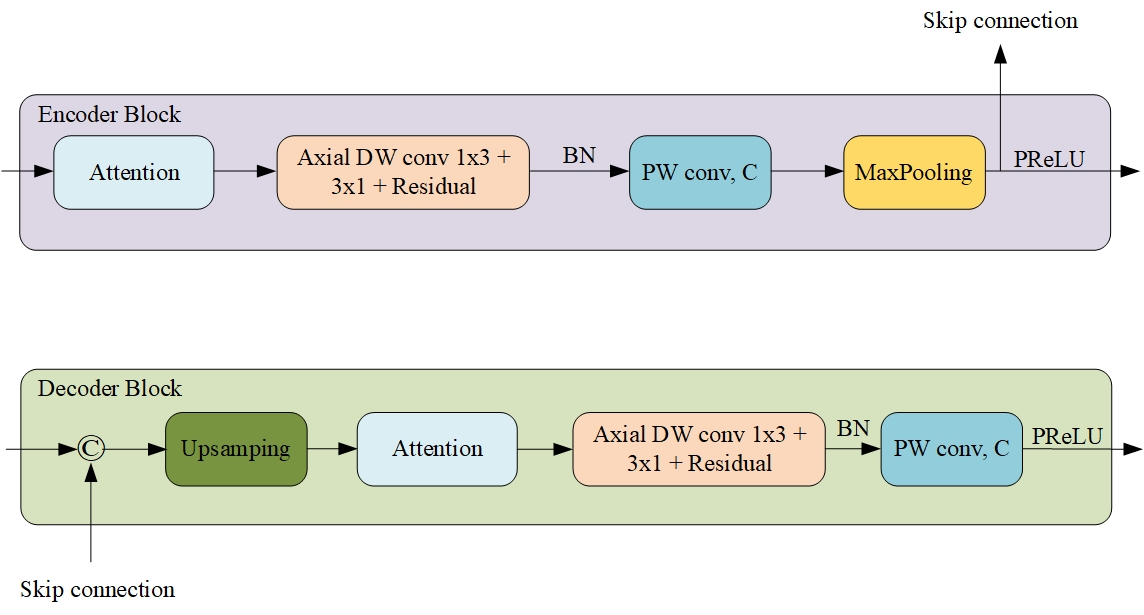
\includegraphics[width=\linewidth]{picture/LLIE/Experiment/Encoder and Decoder}
			\captionsetup{font=scriptsize}
			\caption{Encoder 和 Decoder 的搭配}
			\label{fig: Encoder and Decoder}
		\end{subfigure}
		\begin{subfigure}{0.8\textwidth}
			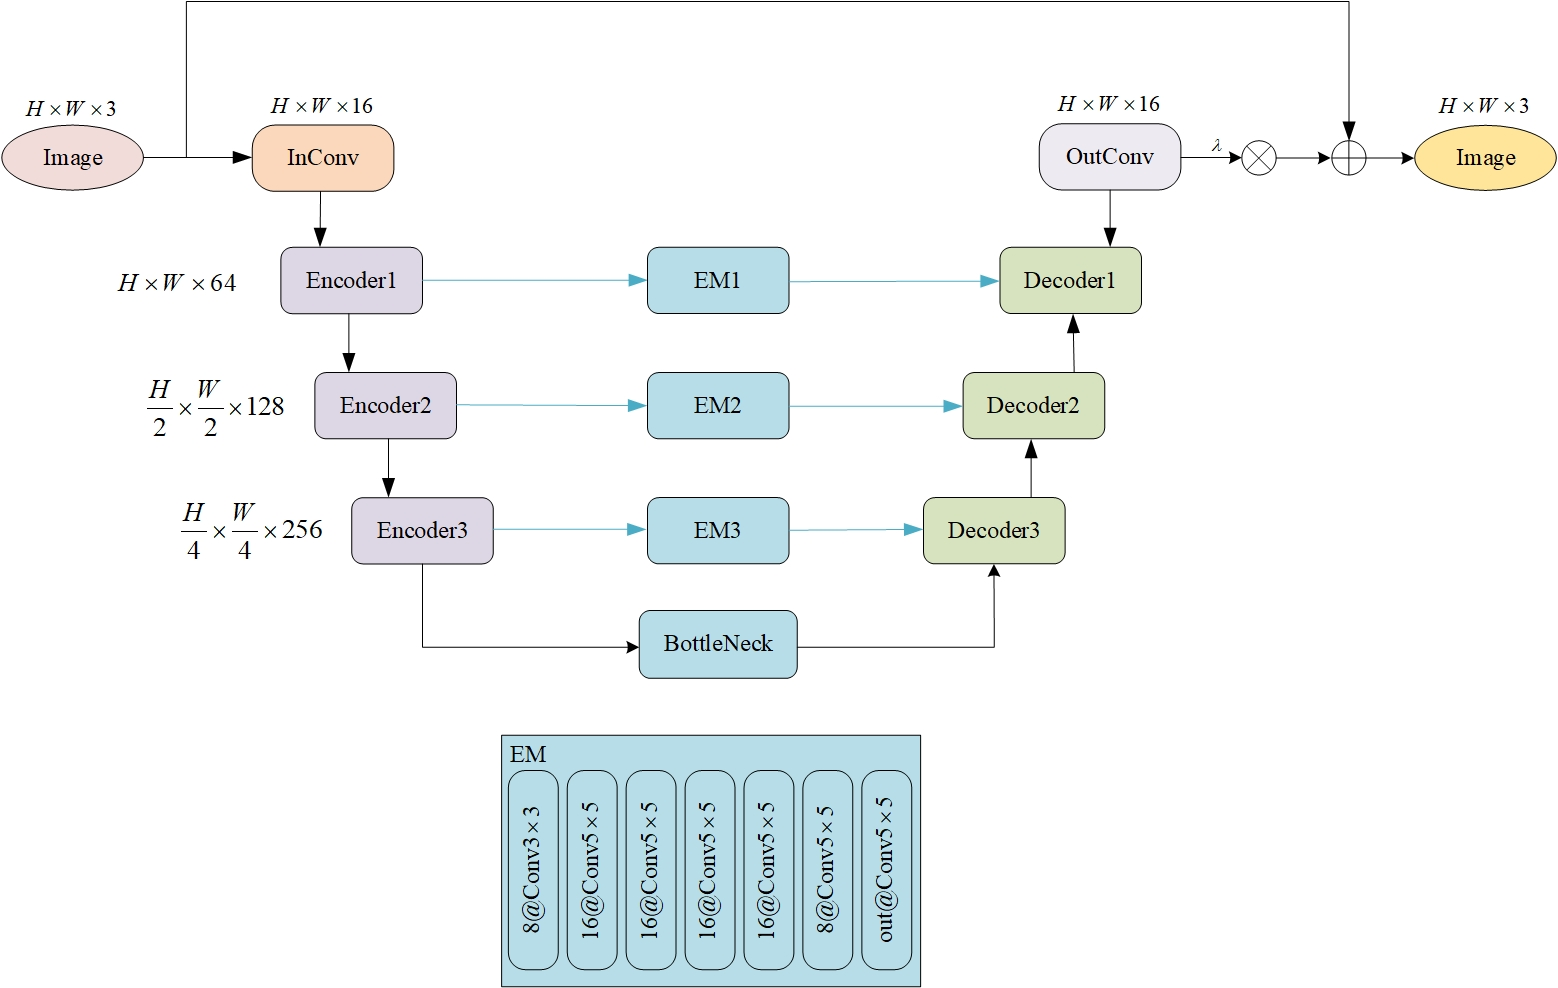
\includegraphics[width=\linewidth]{picture/LLIE/Experiment/Baseline}
			\captionsetup{font=scriptsize}
			\caption{我们提出的U-Net Baseline}
			\label{fig: Baseline}
		\end{subfigure}
	\end{figure}
	
	我们使用 MBLLEN\cite{lv2018mbllen} 中的 EM 模块,旨在加强每个层级中Encoder和Decoder之间的特征连接,从而增强模型的表现能力,如图\ref{fig: Baseline} 所示。
	
	
	我们将激活函数修改为 ReLU 和 PReLU, 其中可视化结果分别如图\ref{fig: Baseline_ReLU} 和 图\ref{fig: Baseline_PReLU} 所示。
	
	\begin{figure}[htbp]
		\centering
		\begin{subfigure}{0.45\textwidth}
			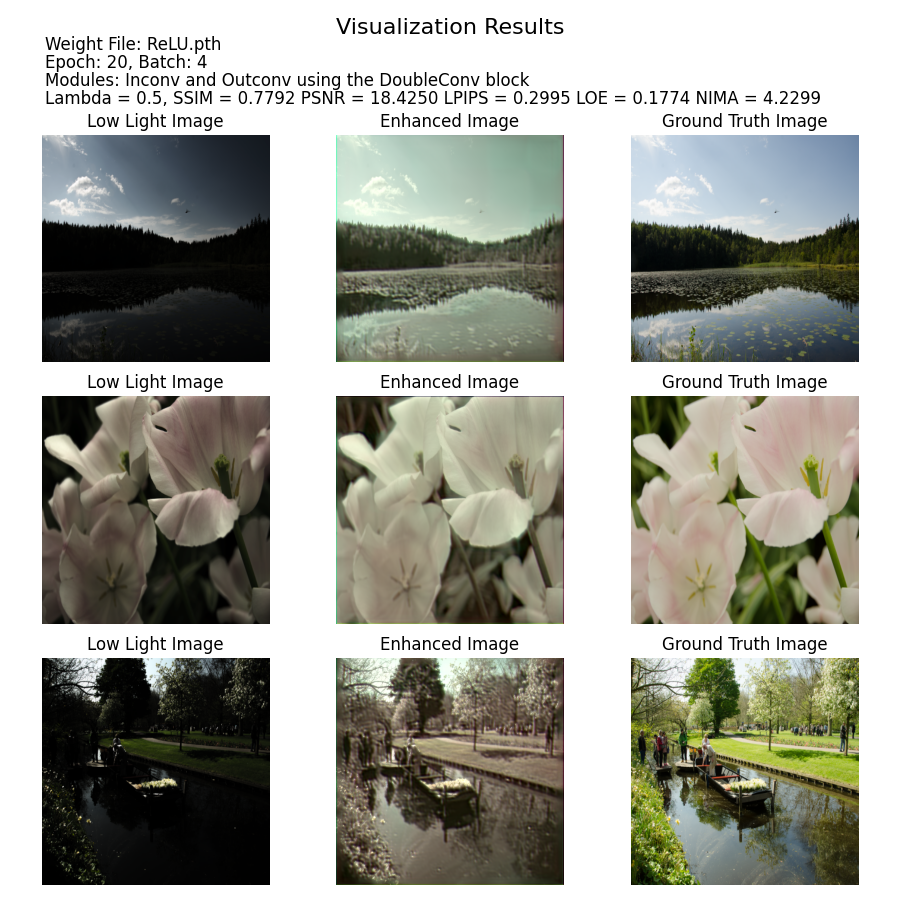
\includegraphics[width=\linewidth]{picture/LLIE/Experiment/myplot_UNet_ReLU}
			\captionsetup{font=scriptsize}
			\caption{ReLU}
			\label{fig: Baseline_ReLU}	
		\end{subfigure}
		\begin{subfigure}{0.45\textwidth}
			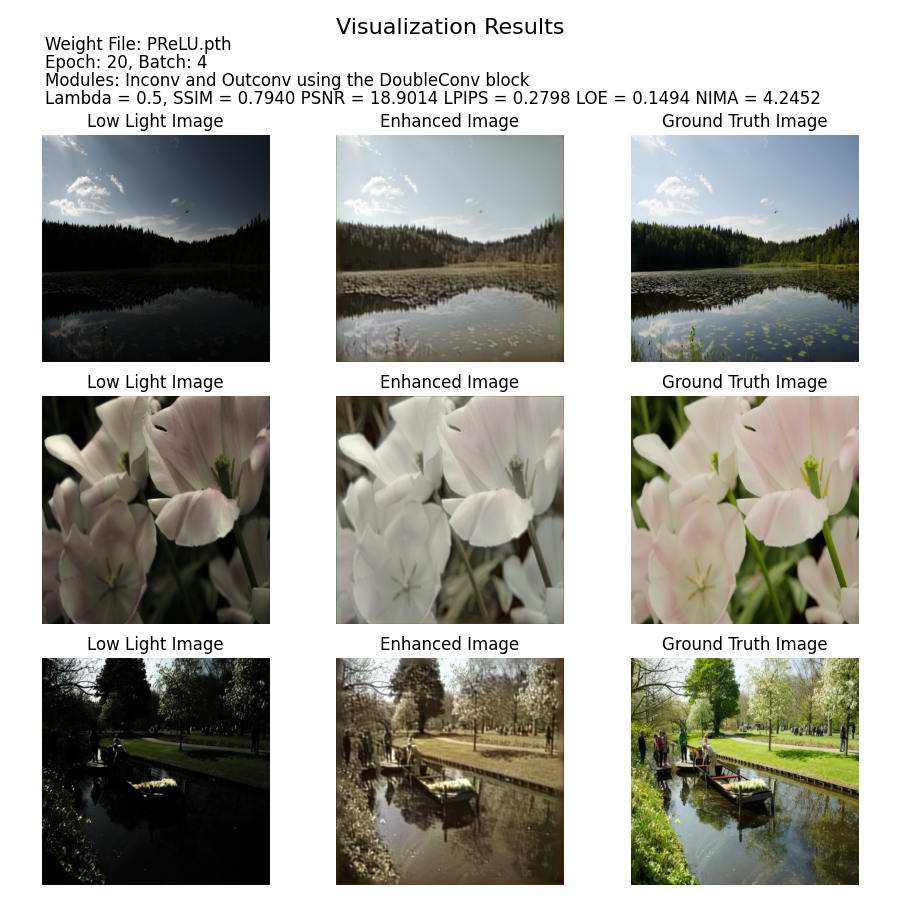
\includegraphics[width=\linewidth]{picture/LLIE/Experiment/myplot_UNet_PReLU}
			\captionsetup{font=scriptsize}
			\caption{PReLU}
			\label{fig: Baseline_PReLU}	
		\end{subfigure}
	\end{figure}
	
	\subsection{其他创新改进}
	
	%		\subsubsection{已知的点}
	
	%		\begin{itemize}
		%			\item{(1)}
		%			一般而言先使用残差块或改进的残差块再使用 Attention 块,主要是为了更好地进行跨通道和空间信息融合。
		%			
		%			\item{(2)}
		%			如果要做得更好,加入结构化先验最终的效果可能会更好。
		%			
		%			\item{(3)}
		%			目前只是针对残差网络上的改进可能意义不大,改进点更多聚焦于\textbf{特征提取能力},\textbf{模型轻量化},
		%			特征提取能力可以关注一下\textbf{图像超分或图像分割领域的算法,这些领域有针对于特征提取能力的一些相关研究}
		%		\end{itemize}
	
	\subsubsection{针对损失函数的改进}
	
	添加平滑度损失(Total Variation Loss)\cite{rudin1992nonlinear}, 受噪声污染的图像的总变分比无噪图像的总变分明显的大, 最小化TV理论上就可以最小化噪声。我们考虑到增强后的图像亮度是不连续的,可能会放大部分噪声,这会降低增强图像的质量,因此采用 TV Loss 约束增强图像。
	
	\begin{equation}
		\begin{aligned}
			\text{Loss}_{\text{TV}} \left( y \right) = \sum_{i=1}^{H} \sum_{j=1}^{W}\sqrt{\left(y_{i,j} - y_{i+1, j}\right)}			
		\end{aligned}
		\label{eq: TV loss}
	\end{equation}
	
	\FloatBarrier
	
	\subsubsection{针对亮度的改进}
	
	\paragraph{LBP}
	
	低光图像和正常光照图像差距体现在像素值上的不同,即低光数值低,正常光数值高,低光图像增强任务可以看作是一个映射(Mapping),这个映射将低光图像重建出正常光的图像,DLN\cite{DLN2020}中提出一种基于反投影理论 (Back-projection) 和注意力机制的但图像低光图像增强方法。作者认为基于深度学习的模型没有办法获得绝对的正常光照(Normal lighting)图像,正常光照图像只是比低光图像像素值高一些,动态范围更大一些。受超分辨\cite{haris2018deep}的思想,希望利用反向投影从低光图像中重建出正常光照图像。 所以作者提出了光反射投影模块(Lighting Back Projection, LBP) (对特征图进行残差学习,增强明亮效果),和特征提取(Feature Aggregation, FA)模块(重新校准特征图特征)。
	
	其中光反射投影模块(LBP)如图\ref{fig: LBP},我们基于光反射投影模块设置了一个并行结构,如图\ref{fig: UNet and LBP} 所示。
	
	\begin{figure}[htbp]
		\centering
		\begin{subfigure}{0.5\textwidth}
			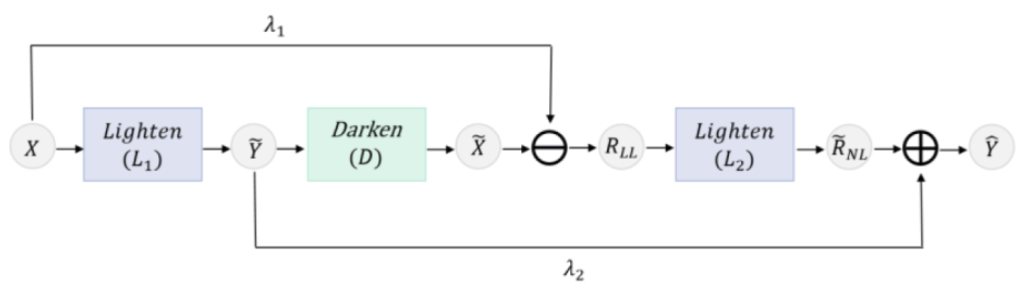
\includegraphics[width=\linewidth]{picture/LLIE/Experiment/LBP}
			\captionsetup{font=scriptsize}
			\caption{Lighting Back Projection}
			\label{fig: LBP}
		\end{subfigure}
		\begin{subfigure}{0.5\textwidth}
			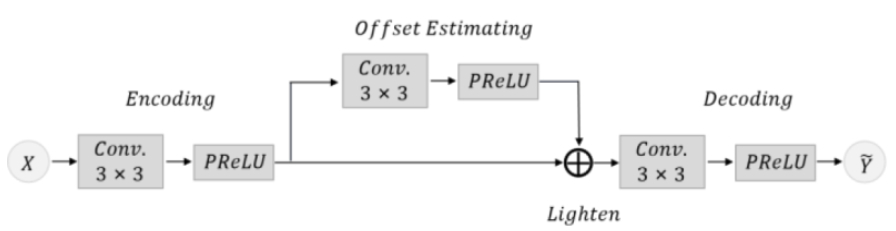
\includegraphics[width=\linewidth]{picture/LLIE/Experiment/Lighten operation}
			\captionsetup{font=scriptsize}
			\caption{Lighten operation}
			\label{fig: Lighten operation}	
		\end{subfigure}
		\begin{subfigure}{0.5\textwidth}
			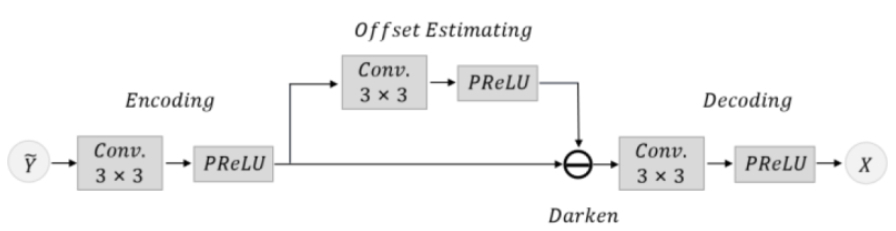
\includegraphics[width=\linewidth]{picture/LLIE/Experiment/Darken operation}
			\captionsetup{font=scriptsize}
			\caption{Darken operation}
			\label{fig: Darken operation}	
		\end{subfigure}
		\caption{图源自\cite{shen2022low}}
	\end{figure}
	
	\begin{figure}[htbp]
		\centering
		\begin{subfigure}{0.8\textwidth}
			\includegraphics[width=\linewidth]{picture/LLIE/Experiment/UNet and LBP}
			\captionsetup{font=scriptsize}
			\caption{UNet and LBP}
			\label{fig: UNet and LBP}
		\end{subfigure}
		\begin{subfigure}{0.8\textwidth}
			\includegraphics[width=\linewidth]{picture/LLIE/Experiment/myplot_LAN}
			\captionsetup{font=scriptsize}
			\caption{Lighten operation}
			\label{fig:myplot_LAN}
		\end{subfigure}
	\end{figure}
	
	增强的结果如图\ref{fig:myplot_LAN}所示。
	
	\paragraph{Zero-DCE} 
	
	低光图片与正常图片之间的一大区别是低光图片中的亮度低的像素占比更高,因此必然存在这样一个函数,这个函数表示如何将一种亮度映射到另一种亮度上,能够使得低光图片中亮度低的像素映射到正常光图像中的对应像素亮度。Zero-DCE 将低光图像到正常光图像的映射问题定义为一个曲线估计问题,通过利用深度学习方法去估计这一函数。Zero-DCE中将这一映射函数称为亮度增强曲线(Light-Enhancement Curve, LE-curve),该曲线满足以下几个原则:
	
	\begin{itemize}
		\item [1)]
		由于亮度值落在区间 $[0, 1]$,为保证亮度值的值域不变,曲线在 0 处值要为 0 ,在 1 处值要为1。
		
		\item [2)]
		曲线必须是单调递增的。不然可能会出现图像中原本较亮的地方反而变暗。
		
		\item [3)]
		曲线必须是可导的。
		
	\end{itemize}
	
	该曲线可以被表示为式\ref{eq: LE-curve}
	
	\begin{equation}
		\begin{aligned}
			LE(I(x); \alpha) = I(x) + \alpha I(x)(1-I(x))
		\end{aligned}
		\label{eq: LE-curve}
	\end{equation}
	
	\subsection{低光边缘推测网络}
	
	我们的主要目标是提升低光图像增强的效果,精确的边缘提取可以提供准确的物体轮廓和边界信息,进而可以作为输入特征帮助低光图像增强任务有效地恢复暗区图像细节和轮廓,使图像更加清晰和易于识别。然而,由于低光图像中普遍存在的边缘弱化问题,会限制图像增强的效果,导致图像的清晰度和细节不足。为了解决低光图像增强任务中暗区细节不足的问题,我们可以通过边缘增强算法提取更接近真实图像的边缘特征,从而改善图像的细节表现和整体质量。低光图像边缘检测算法广泛应用于各种低光照条件下的图像处理任务,如用于自动驾驶领域中的低光照条件下的行人目标检测等任务。
	
	% 应用领域:
	% 无人驾驶:低光条件下提取清晰边缘是自动驾驶汽车准确感知周围环境的关键。精确的边缘信息有助于识别行人、车辆和其他障碍物,确保安全导航。
	% 监控和安全:低光摄像头监控系统依赖于边缘提取技术来识别可疑活动和入侵者。通过提取清晰边缘,可以提高运动检测和对象识别的准确性。低光边缘提取算法有助于提升监控系统的安全性和,预防犯罪和恐怖活动。
	% 医学成像:医学成像(如内窥镜检查和超声波)在低光条件下操作时需要清晰的边缘信息。低光边缘提取技术可提高医学图像的对比度和清晰度,辅助医生诊断和治疗。精确的边缘提取有助于早期发现疾病,提高患者预后。
	% 人工智能:低光边缘提取算法是人工智能视觉系统的核心组成部分。通过提取清晰边缘,人工智能系统可以更准确地识别物体、场景和活动。低光边缘提取技术推动了人工智能技术的进步,使其够在各种光线条件下发挥作用。
	% 增强现实:增强现实设备需要在低光条件下提供准备的边缘检测。低光边缘提取技术确保虚拟物体和现实环境之间流畅的交互。精确的边缘信息增强了增强现实体验,使其更具沉浸感和实用性。
	% 机器视觉:机器视觉系统依赖于边缘提取技术来识别工业缺陷和产品质量问题。低光边缘提取算法提高了机器视觉系统的准确性,确保生产效率和产品质量。低光边缘提取技术在自动化检查和质量控制种发挥着至关重要的作用。
	
	% 应用场景:
	% 计算机视觉:
	%% 图像增强:提高图像对比度,突出边缘信息,便于后续处理。
	%% 目标检测:在低光图像中检测目标,例如行人、车辆等。
	%% 场景理解:解析图像结构,提取场景中的关键边缘信息。
	% 医疗影像:
	%% 医学图像分析:提取医学图像中的病变区域边缘,辅助疾病诊断。
	
	在低光图像中,边缘特征的弱化现象主要源于以下几个方面:
	
	\begin{itemize}
		\item[1)] 
		\textbf{图像噪声增加}:低光环境下,由于光线不足,传感器接收到的光子数量减少,导致图像中的噪声水平显著升高。这些噪声会干扰和掩盖边缘信息,使得边缘检测变得更加困难。此外,噪声引起的伪边缘会混淆真正的边缘,降低边缘检测的准确率。
		
		\item[2)] 
		\textbf{对比度降低}:在低光条件下,图像的对比度显著降低,即亮部与暗部之间的亮度差异变小。这种对比度的降低使得边缘特征与背景的区别不明显,从而增加了边缘提取的难度。
		
		\item[3)] 
		\textbf{图像细节模糊}:低光环境会导致图像细节的模糊。这是由于在光线不足时,光的波长变长,影响了图像的分辨率和清晰度。此外,低光图像的动态范围通常较窄,这意味着图像中亮度值的范围较小,这会导致图像中的高光区域过曝,而暗部区域欠曝,从而丢失边缘信息。这使得边缘信息变得模糊和不清晰,进一步加大了边缘检测的挑战性。
		
		\item[4)]
		\textbf{饱和度降低}:在低光照环境下,图像的色彩饱和度通常会显著降低。这主要是由于光照不足导致色素吸收不充分,进而使得图像中的色彩显得暗淡无光。色彩饱和度的降低进一步减弱了边缘对比度,从而使边缘特征变得难以区分。
		
		
	\end{itemize}
	
	这些因素共同作用,使得低光图像中的边缘特征变得难以识别和提取,从而影响了图像处理和分析的准确性。低光条件下的边缘提取受到信噪比 (SNR) 低的影响,使得提取精确边缘变得困难,采用一些图像预处理技术可以有效提高低光图像的 SNR 和增强边缘特征,有助于低光边缘提取任务。为了解决低光照图像中边缘特征弱化的问题,我们可以从以下四个方面入手:
	
	\begin{itemize}
		\item[1)]
		噪声滤波:应用降噪算法以去除图像中的噪声,从而提高信噪比,增强边缘特征的可见性。
		\item[2)]
		动态范围扩展:通过高动态范围成像 (HDR) 技术扩展图像的动态范围,以恢复丢失的边缘信息。
		\item[3)]
		色彩饱和度增强:利用色彩增强算法提升图像的色彩饱和度,从而提高边缘的对比度。
		\item[4)]
		边缘检测算法:使用专为低光照图像设计的边缘检测算法,以增强算法的鲁棒性和准确性.
	\end{itemize}
	
	这些方法在不同程度上都能有效改善低光照图像的边缘特征,提升图像的整体质量和视觉效果。
	
	传统图像去噪方法,如中值滤波\cite{justusson2006median}和高斯滤波\cite{basu2002gaussian},通过平滑图像来减少噪声。然而,这些方法可能会导致边缘模糊,从而影响边缘提取的准确性。基于非局部均值 (Non-Local Means, NL-Means) 的去噪方法\cite{wilson2013survey}则通过考虑像素间的空间相关性,在去除噪声的同时保留图像的结构和边缘信息。近年来,基于深度学习的去噪方法\cite{tian2020deep}取得了显著进展。这些方法利用卷积神经网络 (Convolutional Neural Networks, CNN) 学习图像中的去噪模式,能够在有效去除噪声的同时保持图像细节。
	
	对比度增强技术,例如直方图均衡化(Histogram Equalization, HE)\cite{stark2000adaptive},是一种常见且简单的对比度增强方法。HE通过重新分配图像的直方图分布来提高图像对比度。然而,HE有时可能会导致过度增强,从而引发不自然的视觉效果。自适应直方图均衡化(Adaptive Histogram Equalization, AHE)\cite{ketcham1974image}是直方图均衡化(HE)的改进版本,它通过考虑图像中的局部区域来避免过度增强现象。局部对比度增强(Local Contrast Enhancement, LCE)是一种较为先进的对比度增强技术。LCE通过在较小区域内增强“局部”对比度,同时防止“全局”对比度的过度提升,从而保护大范围阴影和高光细节。LCE的主要方法是使用大半径和小幅度的反锐化掩膜(Unsharp Masking)来提升局部对比度。伽马校正通过应用非线性函数对图像的像素值进行转换,从而校正图像的对比度和亮度。
	
	边缘检测是整个任务的关键,旨在提取图像中的边缘特征。常用的一些边缘检测算子包括 Sobel 算子,Prewitt 算子,Canny 算子,Laplacian 算子。但基于算子的边缘检测方法由于低光图片的低SNR使得噪声水平与实际边缘特征接近,使得边缘检测算子难以区分真正边缘与噪声干扰。同时,低对比度会减弱边缘特征的显著性,即边缘梯度幅度相应降低,当目标与背景之间的对比度较低时,边缘检测算子难以检测到差异,从而导致边缘提取不准确。低光照条件下的纹理区域会掩盖真实边缘,当纹理与边缘具有相似的强度或方向时,边缘检测算子可能会将纹理错误地识别为边缘,导致边缘提取不准确。
	
	近年来,卷积神经网络(Convolutional Neural Networks, CNNs)在计算机视觉任务中得到了广泛应用。其端到端的特性和强大的特征提取能力使其在图像边缘特征提取任务中表现出色,代表性的模型包括RCF、HED和DexiNed。卷积神经网络通过卷积层和池化层逐级提取图像中的不同层次特征,从低级特征如纹理和边缘,到高级特征如对象形状。在低光条件下,卷积神经网络对噪声的鲁棒性使其能够有效识别出被噪声和模糊掩盖的微弱边缘
	
	基于生成模型的边缘提取技术也逐渐成为最新趋势,例如生成对抗网络(GAN),通过将低光图像作为输入,生成具有增强边缘的图像,从而提高边缘提取的准确性。变分自编码器(Variational Autoencoders, VAE)可以将低光图像编码为潜在表示,然后解码出边缘增强的图像。基于自监督学习的边缘提取算法则利用低光图像中的内在特征,在无需监督的情况下,自动学习并提取图像边缘。
	
	% DexiNed的源码https://github.com/sdoski1/DexiNed/tree/master
	% DexiNed的pytorch源码https://github.com/ParhomEsmaeili/DexiNed-Fine-Tuning-and-Evaluation/blob/main/main_altered.py
	% 用于边缘图评估的matlab源码https://github.com/zeakey/edgeval/blob/master/benchmarkBoundary.m
	% 边缘图评估的依赖工具包https://github.com/pdollar/edges
	%                     https://github.com/pdollar/toolbox/tree/master/channels
	我们利用当前效果比较好的边缘推测网络 DexiNed,并尝试对其进行改进,求解低光图像对应的详细特征,以期后续能够进一步指导低光图像增强,细化恢复的细节。我们的目标是通过一个改进的边缘特征捕获网络能够获取从低光到其边缘特征的有效映射。我们进行了下列尝试,其中模型如图\ref{fig: DCMP} 所示,其中红色箭头是模型训练方向,蓝色箭头是模型的推理过程,其中低光图像 $\mathcal{I}_{i}^{LL}$ 通过 LAN 网络,可以获取初步增强的低光图像 $\mathcal{I}_{i}^{EL}$,表示为 $\mathcal{I}_{i}^{EL} = \mathcal{F}^{LAN} (\mathcal{I}_{i}^{LL})$。LAN 网络由一个三层深度的 U-Net 网络组成,主要实现对低光图像进行简单的亮度增强。
	
	我们将图像边缘推测网络模型表示为 $\mathcal{F}_{i}^{\mathcal{E}}$,其中 $i=1$ 表示使用 DexiNed \cite{Soria_2023}模型,$i=2$ 表示使用 TEED \cite{soria2023tiny}模型,$i=3$ 表示使用 EDTER \cite{pu2022edter}模型 。边缘图像数据集为“正常-边缘”数据对,我们将正常光图像表示为 $\mathcal{N}_{i}$, 对正常光图像进行图像光照退化来模拟低光图像,表示为 $\mathcal{N}_{i}^{dege}$, 依次构建“低光-边缘”数据对,我们将基于边缘图像数据集(“正常-边缘”)构建的“低光-正常-边缘”数据对记为 $\mathcal{D}_{i}^{syn}$,基于低光图像数据集(“低光-正常”)构建的“低光-正常-边缘”数据对记为 $\mathcal{D}_{i}^{low}$。
	
	\begin{itemize}
		\item[1)]
		其中 $\mathcal{D}_{2}^{syn}$ 基于 BIPEDv2 边缘数据集来尝试构建“低光-边缘”数据对,我们利用伽马矫正 (Gamma Correction) 和噪声模拟对 BIPEDv2 中的图像进行图像退化操作,以获取低光图像,进而获取“低光-正常-边缘”训练数据对,如图\ref{fig: degraded} 所示。
		
		\item[2)]
		其中 $\mathcal{D}_{2}^{low}$ 基于 LOLv2 低光数据集来尝试构建“低光-边缘”数据对,我们利用 Canny 算子获取真实图像 (GT) 的边缘特征图片,进而获“低光-正常-边缘”训练数据对。
	\end{itemize}
	
	在边缘推测网络模型的训练中,我们有两种策略可供选择:一种是采用“低光-边缘”训练数据对,另一种是采用“正常-边缘”训练数据对。从一般性的认知来看,低光图像中的语义特征和边缘等特征受光照退化和噪声的影响较大,这使得边缘推测网络从低光数据中捕获边缘特征图的能力大幅减弱。此外,基于深度学习的边缘特征提取网络(如RCF、HED、DexiNed模型)在直接从低光图像中提取边缘特征时,通常效果不佳。这是因为传统的基于编码器的模型主要提取内容特征,这对于生成标准图像(如 sRGB 图像)是足够的,但在详细的结构建模方面表现不足,这些模型通常使用短程操作,如卷积神经网络(CNN),在捕捉低信噪比(SNR)的暗区域的有效表示时效果不佳。因此,采用“低光-边缘”训练数据对可能无法充分利用模型对边缘特征的捕获能力。
	
	为了克服这一问题,我们可以对低光图像进行逆图像退化操作,得到光照相对正常的图像,然后使用“正常-边缘”训练数据对来训练边缘推测网络模型。这种方法有两个显著优势:首先,逆图像退化操作不会扭曲低光图像的纹理和边缘特征,能够很好地保留图像的原始纹理和边缘信息。其次,我们的上游任务是端到端的图像增强任务,这一操作有助于保持端到端模型的整体性和一致性。在我们的实验中,通过对比两种训练策略,我们证明了采用“正常-边缘”训练数据对的有效性。具体来说,通过逆图像退化操作,我们能够更好地保留图像中的重要特征,从而提高边缘推测网络的性能。这不仅在理论上具有合理性,而且在实际实验中也得到了验证。采用“正常-边缘”训练数据对,不仅能够更好地捕获边缘特征,还能增强模型的鲁棒性和泛化能力。因此,针对边缘推测网络模型的训练,使用“正常-边缘”训练数据对是一个更为合理和有效的选择。
	
	我们设计的模型如图\ref{fig: DCMP}所示,可以拓展出以下三种研究思路:
	
	\begin{figure}[htbp]
		\centering
		\includegraphics[width=0.5\linewidth]{picture/Edge Detection/DCMP}
		%\captionsetup{font=scriptsize}
		\caption{边缘特征检测网络}
		\label{fig: DCMP}
	\end{figure}
	
	\begin{itemize}
		\item[1)]
		使用图像 $\mathcal{N}_{i}$ 训练 $\mathcal{F}_{i}^{\mathcal{E}}$ 网络,对图像 $\mathcal{N}_{i}^{dege}$ 使用 $\mathcal{F}_{i}^{\mathcal{E}}$ 进行推理得到边缘结果,这一过程表示为 ${\left[\mathcal{F}\text{-}\alpha\right]}^{\mathcal{E}}_i = {\mathcal{F}}^\mathcal{E}_{i} (\mathcal{N}_{i}^{dege})$;
		
		\item[2)]
		使用图像 $\mathcal{N}_{i}$ 训练 $\mathcal{F}_{i}^{\mathcal{E}}$ 网络,对图像 $\mathcal{N}_{i}^{dege}$ 使用 LAN 增强后使用 $\mathcal{F}_{i}^{\mathcal{E}}$ 进行推理得到边缘结果,这一过程表示为 ${\left[\mathcal{F}\text{-}\beta\right]}^{\mathcal{E}}_i =  \mathcal{F}_{i}^{\mathcal{E}} \left(\mathcal{F}^{LAN} (\mathcal{N}_{i}^{dege})\right)$;
		
		\item[3)]
		使用图像 $\mathcal{N}_{i}$ 训练 $\mathcal{F}_{i}^{\mathcal{E}}$ 网络,对图像 $\mathcal{N}_{i}^{dege}$ 使用 $\mathcal{F}_{i}^{\mathcal{E}}$ 进行推理得到边缘结果,图像 $\mathcal{N}_{i}^{dege}$ 使用 LAN 增强后再使用 $\mathcal{F}_{i}^{\mathcal{E}}$ 进行推理,二者结果相加,这一过程表示为 ${\left[\mathcal{F}\text{-}\gamma\right]}^{\mathcal{E}}_i = \mathcal{F}_{i}^{\mathcal{E}} (\mathcal{N}_{i}^{dege}) + \mathcal{F}_{i}^{\mathcal{E}} \left(\mathcal{F}^{LAN} (\mathcal{N}_{i}^{dege})\right)$.
	\end{itemize}
	
	\begin{figure}[htbp]
		\centering
		\begin{subfigure}{0.02\textwidth}
			\captionsetup{font=scriptsize}
			\caption*{\rotatebox{90}{~~~~~$\gamma$=0.1}}
			\vspace{-2pt}
		\end{subfigure}
		\begin{subfigure}{0.08\textwidth}
			\captionsetup{font=scriptsize}
			\caption*{$\mathcal{N}$= 0.0}
			\includegraphics[width=\linewidth]{picture/Edge Detection/degrade/RGB_001 Gamma=0.1, Gauss Noise=0.0}
			\label{fig: Gamma=0.1, Gauss Noise = 0.0}
		\end{subfigure}
		\begin{subfigure}{0.08\textwidth}
			\captionsetup{font=scriptsize}
			\caption*{$\mathcal{N}$= 0.1}
			\includegraphics[width=\linewidth]{picture/Edge Detection/degrade/RGB_001 Gamma=0.1, Gauss Noise=0.1}
			\label{fig:Gamma=0.1, Gauss Noise = 0.1}
		\end{subfigure}
		\begin{subfigure}{0.08\textwidth}
			\captionsetup{font=scriptsize}
			\caption*{$\mathcal{N}$= 0.2}
			\includegraphics[width=\linewidth]{picture/Edge Detection/degrade/RGB_001 Gamma=0.1, Gauss Noise=0.2}
			\label{fig:Gamma=0.1, Gauss Noise = 0.2}
		\end{subfigure}
		\begin{subfigure}{0.08\textwidth}
			\captionsetup{font=scriptsize}
			\caption*{$\mathcal{N}$= 0.3}
			\includegraphics[width=\linewidth]{picture/Edge Detection/degrade/RGB_001 Gamma=0.1, Gauss Noise=0.3}
			\label{fig:Gamma=0.1, Gauss Noise = 0.3}
		\end{subfigure}
		\begin{subfigure}{0.08\textwidth}
			\captionsetup{font=scriptsize}
			\caption*{$\mathcal{N}$= 0.4}
			\includegraphics[width=\linewidth]{picture/Edge Detection/degrade/RGB_001 Gamma=0.1, Gauss Noise=0.4}
			\label{fig:Gamma=0.1, Gauss Noise = 0.4}
		\end{subfigure}
		\begin{subfigure}{0.08\textwidth}
			\captionsetup{font=scriptsize}
			\caption*{$\mathcal{N}$= 0.5}
			\includegraphics[width=\linewidth]{picture/Edge Detection/degrade/RGB_001 Gamma=0.1, Gauss Noise=0.5}
			\label{fig:Gamma=0.1, Gauss Noise = 0.5}
		\end{subfigure}
		\begin{subfigure}{0.08\textwidth}
			\captionsetup{font=scriptsize}
			\caption*{$\mathcal{N}$= 0.6}
			\includegraphics[width=\linewidth]{picture/Edge Detection/degrade/RGB_001 Gamma=0.1, Gauss Noise=0.6}
			\label{fig:Gamma=0.1, Gauss Noise = 0.6}
		\end{subfigure}
		\begin{subfigure}{0.08\textwidth}
			\captionsetup{font=scriptsize}
			\caption*{$\mathcal{N}$= 0.7}
			\includegraphics[width=\linewidth]{picture/Edge Detection/degrade/RGB_001 Gamma=0.1, Gauss Noise=0.7}
			\label{fig:Gamma=0.1, Gauss Noise = 0.7}
		\end{subfigure}
		\begin{subfigure}{0.08\textwidth}
			\captionsetup{font=scriptsize}
			\caption*{$\mathcal{N}$= 0.8}
			\includegraphics[width=\linewidth]{picture/Edge Detection/degrade/RGB_001 Gamma=0.1, Gauss Noise=0.8}
			\label{fig:Gamma=0.1, Gauss Noise = 0.8}
		\end{subfigure}
		\begin{subfigure}{0.08\textwidth}
			\captionsetup{font=scriptsize}
			\caption*{$\mathcal{N}$= 0.9}
			\includegraphics[width=\linewidth]{picture/Edge Detection/degrade/RGB_001 Gamma=0.1, Gauss Noise=0.9}
			\label{fig:Gamma=0.1, Gauss Noise = 0.9}
		\end{subfigure}
		\begin{subfigure}{0.08\textwidth}
			\captionsetup{font=scriptsize}
			\caption*{$\mathcal{N}$= 1.0}
			\includegraphics[width=\linewidth]{picture/Edge Detection/degrade/RGB_001 Gamma=0.1, Gauss Noise=1.0}
			\label{fig:Gamma=0.1, Gauss Noise = 1.0}
		\end{subfigure}\\
		
		\vspace{-15pt}
		
		\begin{subfigure}{0.02\textwidth}
			\captionsetup{font=scriptsize}
			\caption*{\rotatebox{90}{~~~~~$\gamma$=0.2}}
			\vspace{-2pt}
		\end{subfigure}
		\begin{subfigure}{0.08\textwidth}
			\captionsetup{font=scriptsize}
			%\caption*{$\mathcal{N}$= 0.0}
			\includegraphics[width=\linewidth]{picture/Edge Detection/degrade/RGB_001 Gamma=0.2, Gauss Noise=0.0}
			\label{fig: Gamma=0.2, Gauss Noise = 0.0}
		\end{subfigure}
		\begin{subfigure}{0.08\textwidth}
			\captionsetup{font=scriptsize}
			%\caption*{$\mathcal{N}$= 0.1}
			\includegraphics[width=\linewidth]{picture/Edge Detection/degrade/RGB_001 Gamma=0.2, Gauss Noise=0.1}
			\label{fig:Gamma=0.2, Gauss Noise = 0.1}
		\end{subfigure}
		\begin{subfigure}{0.08\textwidth}
			\captionsetup{font=scriptsize}
			%\caption*{$\mathcal{N}$= 0.2}
			\includegraphics[width=\linewidth]{picture/Edge Detection/degrade/RGB_001 Gamma=0.2, Gauss Noise=0.2}
			\label{fig:Gamma=0.2, Gauss Noise = 0.2}
		\end{subfigure}
		\begin{subfigure}{0.08\textwidth}
			\captionsetup{font=scriptsize}
			%\caption*{$\mathcal{N}$= 0.3}
			\includegraphics[width=\linewidth]{picture/Edge Detection/degrade/RGB_001 Gamma=0.2, Gauss Noise=0.3}
			\label{fig:Gamma=0.2, Gauss Noise = 0.3}
		\end{subfigure}
		\begin{subfigure}{0.08\textwidth}
			\captionsetup{font=scriptsize}
			%\caption*{$\mathcal{N}$= 0.4}
			\includegraphics[width=\linewidth]{picture/Edge Detection/degrade/RGB_001 Gamma=0.2, Gauss Noise=0.4}
			\label{fig:Gamma=0.2, Gauss Noise = 0.4}
		\end{subfigure}
		\begin{subfigure}{0.08\textwidth}
			\captionsetup{font=scriptsize}
			%\caption*{$\mathcal{N}$= 0.5}
			\includegraphics[width=\linewidth]{picture/Edge Detection/degrade/RGB_001 Gamma=0.2, Gauss Noise=0.5}
			\label{fig:Gamma=0.2, Gauss Noise = 0.5}
		\end{subfigure}
		\begin{subfigure}{0.08\textwidth}
			\captionsetup{font=scriptsize}
			%\caption*{$\mathcal{N}$= 0.6}
			\includegraphics[width=\linewidth]{picture/Edge Detection/degrade/RGB_001 Gamma=0.2, Gauss Noise=0.6}
			\label{fig:Gamma=0.2, Gauss Noise = 0.6}
		\end{subfigure}
		\begin{subfigure}{0.08\textwidth}
			\captionsetup{font=scriptsize}
			%\caption*{$\mathcal{N}$= 0.7}
			\includegraphics[width=\linewidth]{picture/Edge Detection/degrade/RGB_001 Gamma=0.2, Gauss Noise=0.7}
			\label{fig:Gamma=0.2, Gauss Noise = 0.7}
		\end{subfigure}
		\begin{subfigure}{0.08\textwidth}
			\captionsetup{font=scriptsize}
			%\caption*{$\mathcal{N}$= 0.8}
			\includegraphics[width=\linewidth]{picture/Edge Detection/degrade/RGB_001 Gamma=0.2, Gauss Noise=0.8}
			\label{fig:Gamma=0.2, Gauss Noise = 0.8}
		\end{subfigure}
		\begin{subfigure}{0.08\textwidth}
			\captionsetup{font=scriptsize}
			%\caption*{$\mathcal{N}$= 0.9}
			\includegraphics[width=\linewidth]{picture/Edge Detection/degrade/RGB_001 Gamma=0.2, Gauss Noise=0.9}
			\label{fig:Gamma=0.2, Gauss Noise = 0.9}
		\end{subfigure}
		\begin{subfigure}{0.08\textwidth}
			\captionsetup{font=scriptsize}
			%\caption*{$\mathcal{N}$= 1.0}
			\includegraphics[width=\linewidth]{picture/Edge Detection/degrade/RGB_001 Gamma=0.2, Gauss Noise=1.0}
			\label{fig:Gamma=0.2, Gauss Noise = 1.0}
		\end{subfigure} \\
		
		\vspace{-15pt}
		
		\begin{subfigure}{0.02\textwidth}
			\captionsetup{font=scriptsize}
			\caption*{\rotatebox{90}{~~~~~$\gamma$=0.3}}
			\vspace{-2pt}
		\end{subfigure}
		\begin{subfigure}{0.08\textwidth}
			\captionsetup{font=scriptsize}
			%\caption*{$\mathcal{N}$= 0.0}
			\includegraphics[width=\linewidth]{picture/Edge Detection/degrade/RGB_001 Gamma=0.3, Gauss Noise=0.0}
			\label{fig: Gamma=0.3, Gauss Noise = 0.0}
		\end{subfigure}
		\begin{subfigure}{0.08\textwidth}
			\captionsetup{font=scriptsize}
			%\caption*{$\mathcal{N}$= 0.1}
			\includegraphics[width=\linewidth]{picture/Edge Detection/degrade/RGB_001 Gamma=0.3, Gauss Noise=0.1}
			\label{fig:Gamma=0.3, Gauss Noise = 0.1}
		\end{subfigure}
		\begin{subfigure}{0.08\textwidth}
			\captionsetup{font=scriptsize}
			%\caption*{$\mathcal{N}$= 0.2}
			\includegraphics[width=\linewidth]{picture/Edge Detection/degrade/RGB_001 Gamma=0.3, Gauss Noise=0.2}
			\label{fig:Gamma=0.3, Gauss Noise = 0.2}
		\end{subfigure}
		\begin{subfigure}{0.08\textwidth}
			\captionsetup{font=scriptsize}
			%\caption*{$\mathcal{N}$= 0.3}
			\includegraphics[width=\linewidth]{picture/Edge Detection/degrade/RGB_001 Gamma=0.3, Gauss Noise=0.3}
			\label{fig:Gamma=0.3, Gauss Noise = 0.3}
		\end{subfigure}
		\begin{subfigure}{0.08\textwidth}
			\captionsetup{font=scriptsize}
			%\caption*{$\mathcal{N}$= 0.4}
			\includegraphics[width=\linewidth]{picture/Edge Detection/degrade/RGB_001 Gamma=0.3, Gauss Noise=0.4}
			\label{fig:Gamma=0.3, Gauss Noise = 0.4}
		\end{subfigure}
		\begin{subfigure}{0.08\textwidth}
			\captionsetup{font=scriptsize}
			%\caption*{$\mathcal{N}$= 0.5}
			\includegraphics[width=\linewidth]{picture/Edge Detection/degrade/RGB_001 Gamma=0.3, Gauss Noise=0.5}
			\label{fig:Gamma=0.3, Gauss Noise = 0.5}
		\end{subfigure}
		\begin{subfigure}{0.08\textwidth}
			\captionsetup{font=scriptsize}
			%\caption*{$\mathcal{N}$= 0.6}
			\includegraphics[width=\linewidth]{picture/Edge Detection/degrade/RGB_001 Gamma=0.3, Gauss Noise=0.6}
			\label{fig:Gamma=0.3, Gauss Noise = 0.6}
		\end{subfigure}
		\begin{subfigure}{0.08\textwidth}
			\captionsetup{font=scriptsize}
			%\caption*{$\mathcal{N}$= 0.7}
			\includegraphics[width=\linewidth]{picture/Edge Detection/degrade/RGB_001 Gamma=0.3, Gauss Noise=0.7}
			\label{fig:Gamma=0.3, Gauss Noise = 0.7}
		\end{subfigure}
		\begin{subfigure}{0.08\textwidth}
			\captionsetup{font=scriptsize}
			%\caption*{$\mathcal{N}$= 0.8}
			\includegraphics[width=\linewidth]{picture/Edge Detection/degrade/RGB_001 Gamma=0.3, Gauss Noise=0.8}
			\label{fig:Gamma=0.3, Gauss Noise = 0.8}
		\end{subfigure}
		\begin{subfigure}{0.08\textwidth}
			\captionsetup{font=scriptsize}
			%\caption*{$\mathcal{N}$= 0.9}
			\includegraphics[width=\linewidth]{picture/Edge Detection/degrade/RGB_001 Gamma=0.3, Gauss Noise=0.9}
			\label{fig:Gamma=0.3, Gauss Noise = 0.9}
		\end{subfigure}
		\begin{subfigure}{0.08\textwidth}
			\captionsetup{font=scriptsize}
			%\caption*{$\mathcal{N}$= 1.0}
			\includegraphics[width=\linewidth]{picture/Edge Detection/degrade/RGB_001 Gamma=0.3, Gauss Noise=1.0}
			\label{fig:Gamma=0.3, Gauss Noise = 1.0}
		\end{subfigure} \\
		
		\vspace{-15pt}
		
		\begin{subfigure}{0.02\textwidth}
			\captionsetup{font=scriptsize}
			\caption*{\rotatebox{90}{~~~~~$\gamma$=0.4}}
			\vspace{-2pt}
		\end{subfigure}
		\begin{subfigure}{0.08\textwidth}
			\captionsetup{font=scriptsize}
			%\caption*{$\mathcal{N}$= 0.0}
			\includegraphics[width=\linewidth]{picture/Edge Detection/degrade/RGB_001 Gamma=0.4, Gauss Noise=0.0}
			\label{fig: Gamma=0.4, Gauss Noise = 0.0}
		\end{subfigure}
		\begin{subfigure}{0.08\textwidth}
			\captionsetup{font=scriptsize}
			%\caption*{$\mathcal{N}$= 0.1}
			\includegraphics[width=\linewidth]{picture/Edge Detection/degrade/RGB_001 Gamma=0.4, Gauss Noise=0.1}
			\label{fig:Gamma=0.4, Gauss Noise = 0.1}
		\end{subfigure}
		\begin{subfigure}{0.08\textwidth}
			\captionsetup{font=scriptsize}
			%\caption*{$\mathcal{N}$= 0.2}
			\includegraphics[width=\linewidth]{picture/Edge Detection/degrade/RGB_001 Gamma=0.4, Gauss Noise=0.2}
			\label{fig:Gamma=0.4, Gauss Noise = 0.2}
		\end{subfigure}
		\begin{subfigure}{0.08\textwidth}
			\captionsetup{font=scriptsize}
			%\caption*{$\mathcal{N}$= 0.3}
			\includegraphics[width=\linewidth]{picture/Edge Detection/degrade/RGB_001 Gamma=0.4, Gauss Noise=0.3}
			\label{fig:Gamma=0.4, Gauss Noise = 0.3}
		\end{subfigure}
		\begin{subfigure}{0.08\textwidth}
			\captionsetup{font=scriptsize}
			%\caption*{$\mathcal{N}$= 0.4}
			\includegraphics[width=\linewidth]{picture/Edge Detection/degrade/RGB_001 Gamma=0.4, Gauss Noise=0.4}
			\label{fig:Gamma=0.4, Gauss Noise = 0.4}
		\end{subfigure}
		\begin{subfigure}{0.08\textwidth}
			\captionsetup{font=scriptsize}
			%\caption*{$\mathcal{N}$= 0.5}
			\includegraphics[width=\linewidth]{picture/Edge Detection/degrade/RGB_001 Gamma=0.4, Gauss Noise=0.5}
			\label{fig:Gamma=0.4, Gauss Noise = 0.5}
		\end{subfigure}
		\begin{subfigure}{0.08\textwidth}
			\captionsetup{font=scriptsize}
			%\caption*{$\mathcal{N}$= 0.6}
			\includegraphics[width=\linewidth]{picture/Edge Detection/degrade/RGB_001 Gamma=0.4, Gauss Noise=0.6}
			\label{fig:Gamma=0.4, Gauss Noise = 0.6}
		\end{subfigure}
		\begin{subfigure}{0.08\textwidth}
			\captionsetup{font=scriptsize}
			%\caption*{$\mathcal{N}$= 0.7}
			\includegraphics[width=\linewidth]{picture/Edge Detection/degrade/RGB_001 Gamma=0.4, Gauss Noise=0.7}
			\label{fig:Gamma=0.4, Gauss Noise = 0.7}
		\end{subfigure}
		\begin{subfigure}{0.08\textwidth}
			\captionsetup{font=scriptsize}
			%\caption*{$\mathcal{N}$= 0.8}
			\includegraphics[width=\linewidth]{picture/Edge Detection/degrade/RGB_001 Gamma=0.4, Gauss Noise=0.8}
			\label{fig:Gamma=0.4, Gauss Noise = 0.8}
		\end{subfigure}
		\begin{subfigure}{0.08\textwidth}
			\captionsetup{font=scriptsize}
			%\caption*{$\mathcal{N}$= 0.9}
			\includegraphics[width=\linewidth]{picture/Edge Detection/degrade/RGB_001 Gamma=0.4, Gauss Noise=0.9}
			\label{fig:Gamma=0.4, Gauss Noise = 0.9}
		\end{subfigure}
		\begin{subfigure}{0.08\textwidth}
			\captionsetup{font=scriptsize}
			%\caption*{$\mathcal{N}$= 1.0}
			\includegraphics[width=\linewidth]{picture/Edge Detection/degrade/RGB_001 Gamma=0.4, Gauss Noise=1.0}
			\label{fig:Gamma=0.4, Gauss Noise = 1.0}
		\end{subfigure} \\
		
		\vspace{-15pt}
		
		\begin{subfigure}{0.02\textwidth}
			\captionsetup{font=scriptsize}
			\caption*{\rotatebox{90}{~~~~~$\gamma$=0.5}}
			\vspace{-2pt}
		\end{subfigure}
		\begin{subfigure}{0.08\textwidth}
			\captionsetup{font=scriptsize}
			%\caption*{$\mathcal{N}$= 0.0}
			\includegraphics[width=\linewidth]{picture/Edge Detection/degrade/RGB_001 Gamma=0.5, Gauss Noise=0.0}
			\label{fig: Gamma=0.5, Gauss Noise = 0.0}
		\end{subfigure}
		\begin{subfigure}{0.08\textwidth}
			\captionsetup{font=scriptsize}
			%\caption*{$\mathcal{N}$= 0.1}
			\includegraphics[width=\linewidth]{picture/Edge Detection/degrade/RGB_001 Gamma=0.5, Gauss Noise=0.1}
			\label{fig:Gamma=0.5, Gauss Noise = 0.1}
		\end{subfigure}
		\begin{subfigure}{0.08\textwidth}
			\captionsetup{font=scriptsize}
			%\caption*{$\mathcal{N}$= 0.2}
			\includegraphics[width=\linewidth]{picture/Edge Detection/degrade/RGB_001 Gamma=0.5, Gauss Noise=0.2}
			\label{fig:Gamma=0.5, Gauss Noise = 0.2}
		\end{subfigure}
		\begin{subfigure}{0.08\textwidth}
			\captionsetup{font=scriptsize}
			%\caption*{$\mathcal{N}$= 0.3}
			\includegraphics[width=\linewidth]{picture/Edge Detection/degrade/RGB_001 Gamma=0.5, Gauss Noise=0.3}
			\label{fig:Gamma=0.5, Gauss Noise = 0.3}
		\end{subfigure}
		\begin{subfigure}{0.08\textwidth}
			\captionsetup{font=scriptsize}
			%\caption*{$\mathcal{N}$= 0.4}
			\includegraphics[width=\linewidth]{picture/Edge Detection/degrade/RGB_001 Gamma=0.5, Gauss Noise=0.4}
			\label{fig:Gamma=0.5, Gauss Noise = 0.4}
		\end{subfigure}
		\begin{subfigure}{0.08\textwidth}
			\captionsetup{font=scriptsize}
			%\caption*{$\mathcal{N}$= 0.5}
			\includegraphics[width=\linewidth]{picture/Edge Detection/degrade/RGB_001 Gamma=0.5, Gauss Noise=0.5}
			\label{fig:Gamma=0.5, Gauss Noise = 0.5}
		\end{subfigure}
		\begin{subfigure}{0.08\textwidth}
			\captionsetup{font=scriptsize}
			%\caption*{$\mathcal{N}$= 0.6}
			\includegraphics[width=\linewidth]{picture/Edge Detection/degrade/RGB_001 Gamma=0.5, Gauss Noise=0.6}
			\label{fig:Gamma=0.5, Gauss Noise = 0.6}
		\end{subfigure}
		\begin{subfigure}{0.08\textwidth}
			\captionsetup{font=scriptsize}
			%\caption*{$\mathcal{N}$= 0.7}
			\includegraphics[width=\linewidth]{picture/Edge Detection/degrade/RGB_001 Gamma=0.5, Gauss Noise=0.7}
			\label{fig:Gamma=0.5, Gauss Noise = 0.7}
		\end{subfigure}
		\begin{subfigure}{0.08\textwidth}
			\captionsetup{font=scriptsize}
			%\caption*{$\mathcal{N}$= 0.8}
			\includegraphics[width=\linewidth]{picture/Edge Detection/degrade/RGB_001 Gamma=0.5, Gauss Noise=0.8}
			\label{fig:Gamma=0.5, Gauss Noise = 0.8}
		\end{subfigure}
		\begin{subfigure}{0.08\textwidth}
			\captionsetup{font=scriptsize}
			%\caption*{$\mathcal{N}$= 0.9}
			\includegraphics[width=\linewidth]{picture/Edge Detection/degrade/RGB_001 Gamma=0.5, Gauss Noise=0.9}
			\label{fig:Gamma=0.5, Gauss Noise = 0.9}
		\end{subfigure}
		\begin{subfigure}{0.08\textwidth}
			\captionsetup{font=scriptsize}
			%\caption*{$\mathcal{N}$= 1.0}
			\includegraphics[width=\linewidth]{picture/Edge Detection/degrade/RGB_001 Gamma=0.5, Gauss Noise=1.0}
			\label{fig:Gamma=0.5, Gauss Noise = 1.0}
		\end{subfigure} \\
		
		\vspace{-15pt}
		
		\begin{subfigure}{0.02\textwidth}
			\captionsetup{font=scriptsize}
			\caption*{\rotatebox{90}{~~~~~$\gamma$=0.6}}
			\vspace{-2pt}
		\end{subfigure}
		\begin{subfigure}{0.08\textwidth}
			\captionsetup{font=scriptsize}
			%\caption*{$\mathcal{N}$= 0.0}
			\includegraphics[width=\linewidth]{picture/Edge Detection/degrade/RGB_001 Gamma=0.6, Gauss Noise=0.0}
			\label{fig: Gamma=0.6, Gauss Noise = 0.0}
		\end{subfigure}
		\begin{subfigure}{0.08\textwidth}
			\captionsetup{font=scriptsize}
			%\caption*{$\mathcal{N}$= 0.1}
			\includegraphics[width=\linewidth]{picture/Edge Detection/degrade/RGB_001 Gamma=0.6, Gauss Noise=0.1}
			\label{fig:Gamma=0.6, Gauss Noise = 0.1}
		\end{subfigure}
		\begin{subfigure}{0.08\textwidth}
			\captionsetup{font=scriptsize}
			%\caption*{$\mathcal{N}$= 0.2}
			\includegraphics[width=\linewidth]{picture/Edge Detection/degrade/RGB_001 Gamma=0.6, Gauss Noise=0.2}
			\label{fig:Gamma=0.6, Gauss Noise = 0.2}
		\end{subfigure}
		\begin{subfigure}{0.08\textwidth}
			\captionsetup{font=scriptsize}
			%\caption*{$\mathcal{N}$= 0.3}
			\includegraphics[width=\linewidth]{picture/Edge Detection/degrade/RGB_001 Gamma=0.6, Gauss Noise=0.3}
			\label{fig:Gamma=0.6, Gauss Noise = 0.3}
		\end{subfigure}
		\begin{subfigure}{0.08\textwidth}
			\captionsetup{font=scriptsize}
			%\caption*{$\mathcal{N}$= 0.4}
			\includegraphics[width=\linewidth]{picture/Edge Detection/degrade/RGB_001 Gamma=0.6, Gauss Noise=0.4}
			\label{fig:Gamma=0.6, Gauss Noise = 0.4}
		\end{subfigure}
		\begin{subfigure}{0.08\textwidth}
			\captionsetup{font=scriptsize}
			%\caption*{$\mathcal{N}$= 0.5}
			\includegraphics[width=\linewidth]{picture/Edge Detection/degrade/RGB_001 Gamma=0.6, Gauss Noise=0.5}
			\label{fig:Gamma=0.6, Gauss Noise = 0.5}
		\end{subfigure}
		\begin{subfigure}{0.08\textwidth}
			\captionsetup{font=scriptsize}
			%\caption*{$\mathcal{N}$= 0.6}
			\includegraphics[width=\linewidth]{picture/Edge Detection/degrade/RGB_001 Gamma=0.6, Gauss Noise=0.6}
			\label{fig:Gamma=0.6, Gauss Noise = 0.6}
		\end{subfigure}
		\begin{subfigure}{0.08\textwidth}
			\captionsetup{font=scriptsize}
			%\caption*{$\mathcal{N}$= 0.7}
			\includegraphics[width=\linewidth]{picture/Edge Detection/degrade/RGB_001 Gamma=0.6, Gauss Noise=0.7}
			\label{fig:Gamma=0.6, Gauss Noise = 0.7}
		\end{subfigure}
		\begin{subfigure}{0.08\textwidth}
			\captionsetup{font=scriptsize}
			%\caption*{$\mathcal{N}$= 0.8}
			\includegraphics[width=\linewidth]{picture/Edge Detection/degrade/RGB_001 Gamma=0.6, Gauss Noise=0.8}
			\label{fig:Gamma=0.6, Gauss Noise = 0.8}
		\end{subfigure}
		\begin{subfigure}{0.08\textwidth}
			\captionsetup{font=scriptsize}
			%\caption*{$\mathcal{N}$= 0.9}
			\includegraphics[width=\linewidth]{picture/Edge Detection/degrade/RGB_001 Gamma=0.6, Gauss Noise=0.9}
			\label{fig:Gamma=0.6, Gauss Noise = 0.9}
		\end{subfigure}
		\begin{subfigure}{0.08\textwidth}
			\captionsetup{font=scriptsize}
			%\caption*{$\mathcal{N}$= 1.0}
			\includegraphics[width=\linewidth]{picture/Edge Detection/degrade/RGB_001 Gamma=0.6, Gauss Noise=1.0}
			\label{fig:Gamma=0.6, Gauss Noise = 1.0}
		\end{subfigure} \\
		
		\vspace{-15pt}
		
		\begin{subfigure}{0.02\textwidth}
			\captionsetup{font=scriptsize}
			\caption*{\rotatebox{90}{~~~~~$\gamma$=0.7}}
			\vspace{-2pt}
		\end{subfigure}
		\begin{subfigure}{0.08\textwidth}
			\captionsetup{font=scriptsize}
			%\caption*{$\mathcal{N}$= 0.0}
			\includegraphics[width=\linewidth]{picture/Edge Detection/degrade/RGB_001 Gamma=0.7, Gauss Noise=0.0}
			\label{fig: Gamma=0.7, Gauss Noise = 0.0}
		\end{subfigure}
		\begin{subfigure}{0.08\textwidth}
			\captionsetup{font=scriptsize}
			%\caption*{$\mathcal{N}$= 0.1}
			\includegraphics[width=\linewidth]{picture/Edge Detection/degrade/RGB_001 Gamma=0.7, Gauss Noise=0.1}
			\label{fig:Gamma=0.7, Gauss Noise = 0.1}
		\end{subfigure}
		\begin{subfigure}{0.08\textwidth}
			\captionsetup{font=scriptsize}
			%\caption*{$\mathcal{N}$= 0.2}
			\includegraphics[width=\linewidth]{picture/Edge Detection/degrade/RGB_001 Gamma=0.7, Gauss Noise=0.2}
			\label{fig:Gamma=0.7, Gauss Noise = 0.2}
		\end{subfigure}
		\begin{subfigure}{0.08\textwidth}
			\captionsetup{font=scriptsize}
			%\caption*{$\mathcal{N}$= 0.3}
			\includegraphics[width=\linewidth]{picture/Edge Detection/degrade/RGB_001 Gamma=0.7, Gauss Noise=0.3}
			\label{fig:Gamma=0.7, Gauss Noise = 0.3}
		\end{subfigure}
		\begin{subfigure}{0.08\textwidth}
			\captionsetup{font=scriptsize}
			%\caption*{$\mathcal{N}$= 0.4}
			\includegraphics[width=\linewidth]{picture/Edge Detection/degrade/RGB_001 Gamma=0.7, Gauss Noise=0.4}
			\label{fig:Gamma=0.7, Gauss Noise = 0.4}
		\end{subfigure}
		\begin{subfigure}{0.08\textwidth}
			\captionsetup{font=scriptsize}
			%\caption*{$\mathcal{N}$= 0.5}
			\includegraphics[width=\linewidth]{picture/Edge Detection/degrade/RGB_001 Gamma=0.7, Gauss Noise=0.5}
			\label{fig:Gamma=0.7, Gauss Noise = 0.5}
		\end{subfigure}
		\begin{subfigure}{0.08\textwidth}
			\captionsetup{font=scriptsize}
			%\caption*{$\mathcal{N}$= 0.6}
			\includegraphics[width=\linewidth]{picture/Edge Detection/degrade/RGB_001 Gamma=0.7, Gauss Noise=0.6}
			\label{fig:Gamma=0.7, Gauss Noise = 0.6}
		\end{subfigure}
		\begin{subfigure}{0.08\textwidth}
			\captionsetup{font=scriptsize}
			%\caption*{$\mathcal{N}$= 0.7}
			\includegraphics[width=\linewidth]{picture/Edge Detection/degrade/RGB_001 Gamma=0.7, Gauss Noise=0.7}
			\label{fig:Gamma=0.7, Gauss Noise = 0.7}
		\end{subfigure}
		\begin{subfigure}{0.08\textwidth}
			\captionsetup{font=scriptsize}
			%\caption*{$\mathcal{N}$= 0.8}
			\includegraphics[width=\linewidth]{picture/Edge Detection/degrade/RGB_001 Gamma=0.7, Gauss Noise=0.8}
			\label{fig:Gamma=0.7, Gauss Noise = 0.8}
		\end{subfigure}
		\begin{subfigure}{0.08\textwidth}
			\captionsetup{font=scriptsize}
			%\caption*{$\mathcal{N}$= 0.9}
			\includegraphics[width=\linewidth]{picture/Edge Detection/degrade/RGB_001 Gamma=0.7, Gauss Noise=0.9}
			\label{fig:Gamma=0.7, Gauss Noise = 0.9}
		\end{subfigure}
		\begin{subfigure}{0.08\textwidth}
			\captionsetup{font=scriptsize}
			%\caption*{$\mathcal{N}$= 1.0}
			\includegraphics[width=\linewidth]{picture/Edge Detection/degrade/RGB_001 Gamma=0.7, Gauss Noise=1.0}
			\label{fig:Gamma=0.7, Gauss Noise = 1.0}
		\end{subfigure} \\
		
		\vspace{-15pt}
		
		\begin{subfigure}{0.02\textwidth}
			\captionsetup{font=scriptsize}
			\caption*{\rotatebox{90}{~~~~~$\gamma$=0.8}}
			\vspace{-2pt}
		\end{subfigure}
		\begin{subfigure}{0.08\textwidth}
			\captionsetup{font=scriptsize}
			%\caption*{$\mathcal{N}$= 0.0}
			\includegraphics[width=\linewidth]{picture/Edge Detection/degrade/RGB_001 Gamma=0.8, Gauss Noise=0.0}
			\label{fig: Gamma=0.8, Gauss Noise = 0.0}
		\end{subfigure}
		\begin{subfigure}{0.08\textwidth}
			\captionsetup{font=scriptsize}
			%\caption*{$\mathcal{N}$= 0.1}
			\includegraphics[width=\linewidth]{picture/Edge Detection/degrade/RGB_001 Gamma=0.8, Gauss Noise=0.1}
			\label{fig:Gamma=0.8, Gauss Noise = 0.1}
		\end{subfigure}
		\begin{subfigure}{0.08\textwidth}
			\captionsetup{font=scriptsize}
			%\caption*{$\mathcal{N}$= 0.2}
			\includegraphics[width=\linewidth]{picture/Edge Detection/degrade/RGB_001 Gamma=0.8, Gauss Noise=0.2}
			\label{fig:Gamma=0.8, Gauss Noise = 0.2}
		\end{subfigure}
		\begin{subfigure}{0.08\textwidth}
			\captionsetup{font=scriptsize}
			%\caption*{$\mathcal{N}$= 0.3}
			\includegraphics[width=\linewidth]{picture/Edge Detection/degrade/RGB_001 Gamma=0.8, Gauss Noise=0.3}
			\label{fig:Gamma=0.8, Gauss Noise = 0.3}
		\end{subfigure}
		\begin{subfigure}{0.08\textwidth}
			\captionsetup{font=scriptsize}
			%\caption*{$\mathcal{N}$= 0.4}
			\includegraphics[width=\linewidth]{picture/Edge Detection/degrade/RGB_001 Gamma=0.8, Gauss Noise=0.4}
			\label{fig:Gamma=0.8, Gauss Noise = 0.4}
		\end{subfigure}
		\begin{subfigure}{0.08\textwidth}
			\captionsetup{font=scriptsize}
			%\caption*{$\mathcal{N}$= 0.5}
			\includegraphics[width=\linewidth]{picture/Edge Detection/degrade/RGB_001 Gamma=0.8, Gauss Noise=0.5}
			\label{fig:Gamma=0.8, Gauss Noise = 0.5}
		\end{subfigure}
		\begin{subfigure}{0.08\textwidth}
			\captionsetup{font=scriptsize}
			%\caption*{$\mathcal{N}$= 0.6}
			\includegraphics[width=\linewidth]{picture/Edge Detection/degrade/RGB_001 Gamma=0.8, Gauss Noise=0.6}
			\label{fig:Gamma=0.8, Gauss Noise = 0.6}
		\end{subfigure}
		\begin{subfigure}{0.08\textwidth}
			\captionsetup{font=scriptsize}
			%\caption*{$\mathcal{N}$= 0.7}
			\includegraphics[width=\linewidth]{picture/Edge Detection/degrade/RGB_001 Gamma=0.8, Gauss Noise=0.7}
			\label{fig:Gamma=0.8, Gauss Noise = 0.7}
		\end{subfigure}
		\begin{subfigure}{0.08\textwidth}
			\captionsetup{font=scriptsize}
			%\caption*{$\mathcal{N}$= 0.8}
			\includegraphics[width=\linewidth]{picture/Edge Detection/degrade/RGB_001 Gamma=0.8, Gauss Noise=0.8}
			\label{fig:Gamma=0.8, Gauss Noise = 0.8}
		\end{subfigure}
		\begin{subfigure}{0.08\textwidth}
			\captionsetup{font=scriptsize}
			%\caption*{$\mathcal{N}$= 0.9}
			\includegraphics[width=\linewidth]{picture/Edge Detection/degrade/RGB_001 Gamma=0.8, Gauss Noise=0.9}
			\label{fig:Gamma=0.8, Gauss Noise = 0.9}
		\end{subfigure}
		\begin{subfigure}{0.08\textwidth}
			\captionsetup{font=scriptsize}
			%\caption*{$\mathcal{N}$= 1.0}
			\includegraphics[width=\linewidth]{picture/Edge Detection/degrade/RGB_001 Gamma=0.8, Gauss Noise=1.0}
			\label{fig:Gamma=0.8, Gauss Noise = 1.0}
		\end{subfigure} \\
		
		\vspace{-15pt}
		
		\begin{subfigure}{0.02\textwidth}
			\captionsetup{font=scriptsize}
			\caption*{\rotatebox{90}{~~~~~$\gamma$=0.9}}
			\vspace{-2pt}
		\end{subfigure}
		\begin{subfigure}{0.08\textwidth}
			\captionsetup{font=scriptsize}
			%\caption*{$\mathcal{N}$= 0.0}
			\includegraphics[width=\linewidth]{picture/Edge Detection/degrade/RGB_001 Gamma=0.9, Gauss Noise=0.0}
			\label{fig: Gamma=0.9, Gauss Noise = 0.0}
		\end{subfigure}
		\begin{subfigure}{0.08\textwidth}
			\captionsetup{font=scriptsize}
			%\caption*{$\mathcal{N}$= 0.1}
			\includegraphics[width=\linewidth]{picture/Edge Detection/degrade/RGB_001 Gamma=0.9, Gauss Noise=0.1}
			\label{fig:Gamma=0.9, Gauss Noise = 0.1}
		\end{subfigure}
		\begin{subfigure}{0.08\textwidth}
			\captionsetup{font=scriptsize}
			%\caption*{$\mathcal{N}$= 0.2}
			\includegraphics[width=\linewidth]{picture/Edge Detection/degrade/RGB_001 Gamma=0.9, Gauss Noise=0.2}
			\label{fig:Gamma=0.9, Gauss Noise = 0.2}
		\end{subfigure}
		\begin{subfigure}{0.08\textwidth}
			\captionsetup{font=scriptsize}
			%\caption*{$\mathcal{N}$= 0.3}
			\includegraphics[width=\linewidth]{picture/Edge Detection/degrade/RGB_001 Gamma=0.9, Gauss Noise=0.3}
			\label{fig:Gamma=0.9, Gauss Noise = 0.3}
		\end{subfigure}
		\begin{subfigure}{0.08\textwidth}
			\captionsetup{font=scriptsize}
			%\caption*{$\mathcal{N}$= 0.4}
			\includegraphics[width=\linewidth]{picture/Edge Detection/degrade/RGB_001 Gamma=0.9, Gauss Noise=0.4}
			\label{fig:Gamma=0.9, Gauss Noise = 0.4}
		\end{subfigure}
		\begin{subfigure}{0.08\textwidth}
			\captionsetup{font=scriptsize}
			%\caption*{$\mathcal{N}$= 0.5}
			\includegraphics[width=\linewidth]{picture/Edge Detection/degrade/RGB_001 Gamma=0.9, Gauss Noise=0.5}
			\label{fig:Gamma=0.9, Gauss Noise = 0.5}
		\end{subfigure}
		\begin{subfigure}{0.08\textwidth}
			\captionsetup{font=scriptsize}
			%\caption*{$\mathcal{N}$= 0.6}
			\includegraphics[width=\linewidth]{picture/Edge Detection/degrade/RGB_001 Gamma=0.9, Gauss Noise=0.6}
			\label{fig:Gamma=0.9, Gauss Noise = 0.6}
		\end{subfigure}
		\begin{subfigure}{0.08\textwidth}
			\captionsetup{font=scriptsize}
			%\caption*{$\mathcal{N}$= 0.7}
			\includegraphics[width=\linewidth]{picture/Edge Detection/degrade/RGB_001 Gamma=0.9, Gauss Noise=0.7}
			\label{fig:Gamma=0.9, Gauss Noise = 0.7}
		\end{subfigure}
		\begin{subfigure}{0.08\textwidth}
			\captionsetup{font=scriptsize}
			%\caption*{$\mathcal{N}$= 0.8}
			\includegraphics[width=\linewidth]{picture/Edge Detection/degrade/RGB_001 Gamma=0.9, Gauss Noise=0.8}
			\label{fig:Gamma=0.9, Gauss Noise = 0.8}
		\end{subfigure}
		\begin{subfigure}{0.08\textwidth}
			\captionsetup{font=scriptsize}
			%\caption*{$\mathcal{N}$= 0.9}
			\includegraphics[width=\linewidth]{picture/Edge Detection/degrade/RGB_001 Gamma=0.9, Gauss Noise=0.9}
			\label{fig:Gamma=0.9, Gauss Noise = 0.9}
		\end{subfigure}
		\begin{subfigure}{0.08\textwidth}
			\captionsetup{font=scriptsize}
			%\caption*{$\mathcal{N}$= 1.0}
			\includegraphics[width=\linewidth]{picture/Edge Detection/degrade/RGB_001 Gamma=0.9, Gauss Noise=1.0}
			\label{fig:Gamma=0.9, Gauss Noise = 1.0}
		\end{subfigure} \\
		
		\vspace{-15pt}
		
		\begin{subfigure}{0.02\textwidth}
			\captionsetup{font=scriptsize}
			\caption*{\rotatebox{90}{~~~~~$\gamma$=1.0}}
			\vspace{-2pt}
		\end{subfigure}
		\begin{subfigure}{0.08\textwidth}
			\captionsetup{font=scriptsize}
			%\caption*{$\mathcal{N}$= 0.0}
			\includegraphics[width=\linewidth]{picture/Edge Detection/degrade/RGB_001 Gamma=1.0, Gauss Noise=0.0}
			\label{fig: Gamma=1.0, Gauss Noise = 0.0}
		\end{subfigure}
		\begin{subfigure}{0.08\textwidth}
			\captionsetup{font=scriptsize}
			%\caption*{$\mathcal{N}$= 0.1}
			\includegraphics[width=\linewidth]{picture/Edge Detection/degrade/RGB_001 Gamma=1.0, Gauss Noise=0.1}
			\label{fig:Gamma=1.0, Gauss Noise = 0.1}
		\end{subfigure}
		\begin{subfigure}{0.08\textwidth}
			\captionsetup{font=scriptsize}
			%\caption*{$\mathcal{N}$= 0.2}
			\includegraphics[width=\linewidth]{picture/Edge Detection/degrade/RGB_001 Gamma=1.0, Gauss Noise=0.2}
			\label{fig:Gamma=1.0, Gauss Noise = 0.2}
		\end{subfigure}
		\begin{subfigure}{0.08\textwidth}
			\captionsetup{font=scriptsize}
			%\caption*{$\mathcal{N}$= 0.3}
			\includegraphics[width=\linewidth]{picture/Edge Detection/degrade/RGB_001 Gamma=1.0, Gauss Noise=0.3}
			\label{fig:Gamma=1.0, Gauss Noise = 0.3}
		\end{subfigure}
		\begin{subfigure}{0.08\textwidth}
			\captionsetup{font=scriptsize}
			%\caption*{$\mathcal{N}$= 0.4}
			\includegraphics[width=\linewidth]{picture/Edge Detection/degrade/RGB_001 Gamma=1.0, Gauss Noise=0.4}
			\label{fig:Gamma=1.0, Gauss Noise = 0.4}
		\end{subfigure}
		\begin{subfigure}{0.08\textwidth}
			\captionsetup{font=scriptsize}
			%\caption*{$\mathcal{N}$= 0.5}
			\includegraphics[width=\linewidth]{picture/Edge Detection/degrade/RGB_001 Gamma=1.0, Gauss Noise=0.5}
			\label{fig:Gamma=1.0, Gauss Noise = 0.5}
		\end{subfigure}
		\begin{subfigure}{0.08\textwidth}
			\captionsetup{font=scriptsize}
			%\caption*{$\mathcal{N}$= 0.6}
			\includegraphics[width=\linewidth]{picture/Edge Detection/degrade/RGB_001 Gamma=1.0, Gauss Noise=0.6}
			\label{fig:Gamma=1.0, Gauss Noise = 0.6}
		\end{subfigure}
		\begin{subfigure}{0.08\textwidth}
			\captionsetup{font=scriptsize}
			%\caption*{$\mathcal{N}$= 0.7}
			\includegraphics[width=\linewidth]{picture/Edge Detection/degrade/RGB_001 Gamma=1.0, Gauss Noise=0.7}
			\label{fig:Gamma=1.0, Gauss Noise = 0.7}
		\end{subfigure}
		\begin{subfigure}{0.08\textwidth}
			\captionsetup{font=scriptsize}
			%\caption*{$\mathcal{N}$= 0.8}
			\includegraphics[width=\linewidth]{picture/Edge Detection/degrade/RGB_001 Gamma=1.0, Gauss Noise=0.8}
			\label{fig:Gamma=1.0, Gauss Noise = 0.8}
		\end{subfigure}
		\begin{subfigure}{0.08\textwidth}
			\captionsetup{font=scriptsize}
			%\caption*{$\mathcal{N}$= 0.9}
			\includegraphics[width=\linewidth]{picture/Edge Detection/degrade/RGB_001 Gamma=1.0, Gauss Noise=0.9}
			\label{fig:Gamma=1.0, Gauss Noise = 0.9}
		\end{subfigure}
		\begin{subfigure}{0.08\textwidth}
			\captionsetup{font=scriptsize}
			%\caption*{$\mathcal{N}$= 1.0}
			\includegraphics[width=\linewidth]{picture/Edge Detection/degrade/RGB_001 Gamma=1.0, Gauss Noise=1.0}
			\label{fig:Gamma=1.0, Gauss Noise = 1.0}
		\end{subfigure} \\
		
		\caption{我们通过矫正 $\gamma$ 值和高斯噪声 $\mathcal{N}$ 以模拟不同程度的图像退化,具体来说,我们将 $\gamma$ 值和 $\mathcal{N}$ 设置为 $\left[ 0, 1\right]$,并列举了各种搭配组合下退化的图像。此外,我们计算了每一种搭配组合下低光数据集的 PSNR 和 SSIM,选取最接近于接近低光数据集的图像退化搭配组合。}
		\label{fig: degraded}
	\end{figure}
	
	\begin{table}
		\centering
		\small
		\resizebox{\textwidth}{!}{ %按照宽度调整调整表格大小
			\begin{tabular}{|>{\centering\arraybackslash}m{3.5cm}|c|c|c|c|c|c|c|c|c|c|c|}
				\hline
				\diagbox{$\gamma$}{SSIM \textbackslash PSNR}{$\mathcal{N}$} & $\mathcal{N} = 0.0$ & $\mathcal{N} = 0.1$ & $\mathcal{N} = 0.2$ & $\mathcal{N} = 0.3$ & $\mathcal{N} = 0.4$ & $\mathcal{N} = 0.5$ & $\mathcal{N} = 0.6$ & $\mathcal{N} = 0.7$ & $\mathcal{N} = 0.8$ & $\mathcal{N} = 0.9$ & $\mathcal{N} = 1.0$\\
				\hline
				$\gamma = 0.1$ & \diagbox{0.1660}{6.1554}  & \diagbox{0.0959}{6.4417}  & \diagbox{0.0606}{6.6640}  & \diagbox{0.0435}{6.7398}  & \diagbox{0.0332}{6.6769}  & \diagbox{0.0266}{6.5347} & \diagbox{0.0222}{6.3718} & \diagbox{0.0190}{6.2156} & \diagbox{0.0167}{6.0778} & \diagbox{0.0150}{5.9585} & \diagbox{0.0136}{5.8565} \\
				\hline
				$\gamma = 0.2$ & \diagbox{0.3415}{8.1001}  & \cellcolor{yellow}\diagbox{0.1521}{8.1968}  & \diagbox{0.0866}{8.1781}  & \diagbox{0.0588}{7.9832}  & \diagbox{0.0436}{7.6728}  & \diagbox{0.0342}{7.3333} & \diagbox{0.0280}{7.0231} & \diagbox{0.0238}{6.7600} & \diagbox{0.0207}{6.5416} & \diagbox{0.0184}{6.3612} & \diagbox{0.0166}{6.2111} \\
				\hline
				$\gamma = 0.3$ & \diagbox{0.5139}{10.1027} & \cellcolor{yellow}\diagbox{0.1990}{9.9589}  & \diagbox{0.1058}{9.5971}  & \diagbox{0.0690}{9.0532}  & \diagbox{0.0498}{8.4615}  & \diagbox{0.0384}{7.9259} & \diagbox{0.0312}{7.4841} & \diagbox{0.0263}{7.1307} & \diagbox{0.0227}{6.8492} & \diagbox{0.0201}{6.6227} & \diagbox{0.0180}{6.4381} \\
				\hline
				$\gamma = 0.4$ & \diagbox{0.6675}{12.2212} & \diagbox{0.2366}{11.7569} & \diagbox{0.1192}{10.9091} & \diagbox{0.0753}{9.9467}  & \diagbox{0.0532}{9.0669}  & \diagbox{0.0406}{8.3538} & \diagbox{0.0326}{7.8023} & \diagbox{0.0273}{7.3798} & \diagbox{0.0235}{7.0517} & \diagbox{0.0207}{6.7924} & \diagbox{0.0186}{6.5837} \\
				\hline
				$\gamma = 0.5$ & \diagbox{0.7917}{14.5296} & \diagbox{0.2646}{13.6013} & \diagbox{0.1279}{12.0932} & \diagbox{0.0787}{10.6659} & \diagbox{0.0548}{9.5171}  & \diagbox{0.0413}{8.6556} & \diagbox{0.0331}{8.0202} & \diagbox{0.0276}{7.5463} & \diagbox{0.0237}{7.1847} & \diagbox{0.0208}{6.9028} & \diagbox{0.0186}{6.6772} \\
				\hline
				$\gamma = 0.6$ & \diagbox{0.8821}{17.1143} & \diagbox{0.2833}{15.4492} & \diagbox{0.1326}{13.0987} & \diagbox{0.0799}{11.2094} & \diagbox{0.0549}{9.8329}  & \diagbox{0.0412}{8.8591} & \diagbox{0.0328}{8.1632} & \diagbox{0.0273}{7.6538} & \diagbox{0.0234}{7.2699} & \diagbox{0.0206}{6.9726} & \diagbox{0.0184}{6.7366} \\
				\hline
				$\gamma = 0.7$ & \diagbox{0.9422}{20.2024} & \diagbox{0.2944}{17.2510} & \diagbox{0.1345}{13.9015} & \diagbox{0.0798}{11.5989} & \diagbox{0.0544}{10.0485} & \diagbox{0.0406}{8.9936} & \diagbox{0.0322}{8.2569} & \diagbox{0.0268}{7.7231} & \diagbox{0.0230}{7.3246} & \diagbox{0.0202}{7.0176} & \diagbox{0.0180}{6.7741} \\
				\hline
				$\gamma = 0.8$ & \diagbox{0.9778}{24.2759} & \diagbox{0.2994}{18.8603} & \diagbox{0.1342}{14.4761} & \diagbox{0.0787}{11.8536} & \diagbox{0.0533}{10.1836} & \diagbox{0.0396}{9.0772} & \diagbox{0.0314}{8.3141} & \diagbox{0.0261}{7.7663} & \diagbox{0.0223}{7.3586} & \diagbox{0.0196}{7.0445} & \diagbox{0.0175}{6.7974} \\
				\hline
				$\gamma = 0.9$ & \diagbox{0.9949}{30.6200} & \diagbox{0.2998}{19.9949} & \diagbox{0.1325}{14.8087} & \diagbox{0.0770}{11.9930} & \diagbox{0.0519}{10.2575} & \diagbox{0.0385}{9.1227} & \diagbox{0.0305}{8.3455} & \diagbox{0.0253}{7.7899} & \diagbox{0.0217}{7.3768} & \diagbox{0.0190}{7.0601} & \diagbox{0.0170}{6.8101} \\
				\hline
				$\gamma = 1.0$ & \diagbox{1}{$\infty$}     & \diagbox{0.2976}{20.4729} & \diagbox{0.1302}{14.9476} & \diagbox{0.0752}{12.0577} & \diagbox{0.0505}{10.2963} & \diagbox{0.0374}{9.1496} & \diagbox{0.0296}{8.3660} & \diagbox{0.0246}{7.8064} & \diagbox{0.0211}{7.3903} & \diagbox{0.0185}{7.0720} & \diagbox{0.0166}{6.8203} \\
				\hline
			\end{tabular}
		}
		\caption{LOL-v2数据集中的Real Captured 的 PSNR 为 8.817 dB, SSIM 为 0.192。我们想要通过计算了每一种 $\gamma$ 值和高斯噪声值 $\mathcal{N}$ 搭配对应的 $\mathcal{D}_{2}^{syn}$ 数据集的 PSNR 和 SSIM,以获取尽可能接近于真实低光数据集的图像退化。我们通过计算这些数据集和真实低光数据集PSNR和SSIM的标准化差值,选取了最接近于接近低光数据集的图像退化搭配组合。我们将 $\gamma$ 值设置为 0.25,$\mathcal{N}$ 设置为 0.1,此时,$\mathcal{D}_{2}^{syn}$ 数据集的 PSNR 为 9.075 dB,SSIM 为 0.1767。}
		% Gamma: 0.25, Noise Level: 0.1
		% Average PSNR: 9.074948466590183
		% Average SSIM: 0.1767813303256974
		\label{tab: degraded}
	\end{table}
	
	在我们早期的研究和实验中,我们观察到基于深度学习的边缘特征提取网络(如RCF、HED、DexiNed模型)在直接从低光图像中提取边缘特征时,通常效果不佳。这是因为传统的基于编码器的模型主要提取内容特征,这对于生成标准图像(如 sRGB图像)是足够的,但在详细的结构建模方面表现不足,这些模型通常使用短程操作,如卷积神经网络(CNN),在捕捉低信噪比(SNR)的暗区域的有效表示时效果不佳。为了改善这种情况,我们设计了一种训练策略,即首先使用$\mathcal{D}^{syn}_2$对DexiNed模型进行训练。这个过程如图\ref{fig: DCMP} 中黄色部分所示。
	
	进一步的实验表明,当我们使用正常光图像对 DexiNed 模型进行训练,然后将相应的低光图像输入到经过训练的 DexiNed 模型中时,可以获得更好的边缘特征提取效果。这不仅在视觉上表现良好,而且在 ODS、OIS 和 AP 等评价指标上也有显著提升。基于这些发现,我们提出了一种有效的方法:首先使用正常光图像训练 DexiNed 模型,然后对低光图像进行初步的增强处理,最后使用训练好的 DexiNed 模型对增强后的低光图像进行推理,以获取边缘特征图。
	
	这种方法的理论基础在于,低光图像在边缘和纹理特征上存在严重退化,传统的边缘提取网络难以直接从中捕获这些特征。然而,通过对光线的适当增强,可以在一定程度上恢复图像的边缘和纹理特征,从而帮助模型更准确地提取边缘信息。因此,利用正常光图像进行模型训练,然后对低光图像进行增强处理,是获取低光图像边缘特征的有效策略。
	
	综上所述,通过我们的研究,我们验证了利用正常光图像训练边缘特征提取模型并对低光图像进行初步增强处理,可以显著改善低光环境下的边缘特征提取效果。这一发现不仅为边缘检测任务提供了新的思路,也为低光图像的处理提供了有效的方法和技术支持。
	
	\subsubsection{实验设计}
	
	对于${\left[\mathcal{F}\text{-}\alpha\right]}^{\mathcal{E}}_1$,我们基于改进的 DexiNed 模型来构建一个生成式对抗网络,以提升低光图像的边缘提取效果;对于${\left[\mathcal{F}\text{-}\beta\right]}^{\mathcal{E}}_1$,我们使用 LAN 网络来恢复图像的亮度和对比度,获取一个初步增强的低光图像,然后使用 DexiNed 模型来提取低光图像的边缘特征。${\left[\mathcal{F}\text{-}\gamma\right]}^{\mathcal{E}}_1$是上述两个分支的合并。实验数据集选取BIPED-v2和LOL-v2,包含训练和测试集的低光图像及其对应的正常光照下的边缘图像。具体的实验设置如下:
	
	\begin{itemize}
		\item[1)]
		硬件环境:实验配置的GPU为 NVIDIA GeForce RTX 4090,CUDA 11.3 用于加速计算。
		\item[2)]
		软件环境:使用 Python 3.11 和 PyTorch 深度学习框架进行模型训练与测试。
	\end{itemize}
	
	我们采用 BDC Loss 损失函数用于生成式对抗网络的生成器损失和 DexiNed 模型损失,判别器使用 $\mathcal{L}_1$ 损失。我们使用 Adam 优化器,初始学习率设置为1e-4,权重衰减设置为1e-8,采用 MultiStepLR 调度器,在第 10 和第 15 个epoch时将学习率分别乘以0.1。训练共进行100个epoch,每个epoch结束时保存模型权重至指定路径。每个epoch内,模型对输入图像进行前向传播计算预测结果,通过反向传播更新模型权重。
	
	\subsubsection{评价指标与结果评估}		
	
	在边缘检测网络评估中,常用的评价指标包括 ODS(Optimal Dataset Scale)、OIS(Optimal Image Scale)、AP(Average Pricision)和R50.
	
	ODS 是指在整个数据集上选取的最佳阈值下的F-measure(F1 Score)。F-measure是精度(Precision)和召回率(Recall)的调和平均数,用于平衡模型的精度和召回率。F1 Score 综合考虑 Precision 和 Recall 的指标,如式.\ref{eq: F1 Score}。Precision (P) 表示模型预测为正的样本中,真正为正的比例。Recall(R) 表示实际为正的样本中,被模型预测为正的比例。ODS表示在所有图像中选择一个全局最佳阈值,使得 F1 Score 最高
	
	\begin{equation}
		\begin{aligned}
			F1 = 2 \cdot \frac{P \cdot R}{P + R}
		\end{aligned}
		\label{eq: F1 Score}
	\end{equation}
	
	OIS 是指在每个图像上分别选取最佳阈值下的平均 F-measure。即对每张图像单独计算最佳阈值下的 F1 Score,然后对所有图像的 F1 Score 求平均。这种方法能够反映在单个图像上的最佳性能,而不受全局阈值的限制。AP是指在不同阈值下计算的Precision和Recall的曲线下面积(Area Under Curve, AUC)。具体步骤如下:
	
	\begin{itemize}
		\item[1)]
		计算在不同阈值下的Precision和Recall;
		\item[2)]
		绘制Precision-Recall曲线;
		\item[3)]
		计算曲线下面积,得到 Average Precision。
	\end{itemize}
	
	AP 反映了模型在各种阈值下的整体性能,能够综合评估模型在精度和召回率之间的权衡情况。
	
	R50表示在召回率达到50\%时的精度。该指标用于评估在中等召回率下模型的精度表现。具体来说,R50的计算步骤如下:
	
	\begin{itemize}
		\item[1)]
		调整阈值,找到使召回率达到50\%的点;
		\item[2)]
		计算对应的精度;
		\item[3)]
		R50反映了在保证召回率的情况下,模型的精度表现情况。
	\end{itemize}
	
	\paragraph{非极大值抑制(NMS)}
	
	深度神经网络输出的边缘一般都比较宽,这是因为图像的边缘常常是灰度值跳跃比较大的地方,这些跳跃比较大的区域常常范围是比较宽的。如果用这个比较宽泛的区域作为边缘,显然会有很大的不足,我们需要使得边缘只有1-2个像素的范围,这样的边缘区域才足够精确。因此,我们在对边缘推测网络的结果进行评估之前需要进行非极大值抑制(Non-maximunm supression, NMS)操作。
	
	%\footnote{https://www.zhihu.com/question/37172820}{https://zhuanlan.zhihu.com/p/549550255}中详细解释了canny算子中的非极大值抑制的基本原理。
	
	
	\begin{table}[!htbp]
		\centering
		\small
		%\resizebox{\textwidth}{!}{ %按照宽度调整调整表格大小
			\begin{tabular}{>{\centering\arraybackslash}m{1.5cm} c c c c c}
				
				\hline
				
				\textbf{Branch} & \textbf{Dataset} & \textbf{ODS} & \textbf{OIS} & \textbf{AP} & \textbf{R50}  \\
				
				\hline
				
				${\left[\mathcal{F}\text{-}\alpha\right]}^{\mathcal{E}}_1$ & LOL-v2  & .863 & .888 & .915 & .997 \\
				
				${\left[\mathcal{F}\text{-}\alpha\right]}^{\mathcal{E}}_1$ & BIPED-v2& .807 & .813 & .871 & .942 \\
				
				${\left[\mathcal{F}\text{-}\beta\right]}^{\mathcal{E}}_1$  & LOL-v2  & .844 & .866 & .795 & .925 \\
				
				${\left[\mathcal{F}\text{-}\beta\right]}^{\mathcal{E}}_1$  & BIPED-v2& .759 & .767 & .800 & .861 \\
				
				${\left[\mathcal{F}\text{-}\gamma\right]}^{\mathcal{E}}_1$ & LOL-v2  & .863 & .888 & .915 & .997 \\
				
				${\left[\mathcal{F}\text{-}\gamma\right]}^{\mathcal{E}}_1$ & BIPED-v2& .807 & .813 & .871 & .942 \\
				
				\hline
				
			\end{tabular}
			%}
		%\captionsetup{font=scriptsize} %设置标题字体与表格字体一致
		\caption{
			\label{tab: Result}
			不同的训练和推理方式的结果} %表格的标题
		
	\end{table}
	
	\begin{figure}[htbp]
		\centering
		\begin{subfigure}{0.16\textwidth}
			\includegraphics[width=\linewidth]{picture/Edge Detection/res(F-α)/Input/RGB_008} \\
			\includegraphics[width=\linewidth]{picture/Edge Detection/res(F-α)/Input/RGB_010} \\
			\includegraphics[width=\linewidth]{picture/Edge Detection/res(F-α)/Input/RGB_017} \\
			\includegraphics[width=\linewidth]{picture/Edge Detection/res(F-α)/Input/RGB_025}
			\caption{Input image}
		\end{subfigure}
		\begin{subfigure}{0.16\textwidth}
			\includegraphics[width=\linewidth]{picture/Edge Detection/res(F-α)/GT/RGB_008} \\
			\includegraphics[width=\linewidth]{picture/Edge Detection/res(F-α)/GT/RGB_010} \\
			\includegraphics[width=\linewidth]{picture/Edge Detection/res(F-α)/GT/RGB_017} \\
			\includegraphics[width=\linewidth]{picture/Edge Detection/res(F-α)/GT/RGB_025}
			\caption{GT image}
		\end{subfigure}
		\begin{subfigure}{0.16\textwidth}
			\includegraphics[width=\linewidth]{picture/Edge Detection/res(F-α)/Predicted Edges/RGB_008} \\
			\includegraphics[width=\linewidth]{picture/Edge Detection/res(F-α)/Predicted Edges/RGB_010} \\
			\includegraphics[width=\linewidth]{picture/Edge Detection/res(F-α)/Predicted Edges/RGB_017} \\
			\includegraphics[width=\linewidth]{picture/Edge Detection/res(F-α)/Predicted Edges/RGB_025}
			\caption{Predicted Edges}
		\end{subfigure}
		\begin{subfigure}{0.16\textwidth}
			\includegraphics[width=\linewidth]{picture/Edge Detection/res(F-α)/Predicted Edges NMS/RGB_008} \\
			\includegraphics[width=\linewidth]{picture/Edge Detection/res(F-α)/Predicted Edges NMS/RGB_010} \\
			\includegraphics[width=\linewidth]{picture/Edge Detection/res(F-α)/Predicted Edges NMS/RGB_017} \\
			\includegraphics[width=\linewidth]{picture/Edge Detection/res(F-α)/Predicted Edges NMS/RGB_025}
			\caption{NMS}
		\end{subfigure}
		\begin{subfigure}{0.16\textwidth}
			\includegraphics[width=\linewidth]{picture/Edge Detection/res(F-α)/GT Edges/RGB_008} \\
			\includegraphics[width=\linewidth]{picture/Edge Detection/res(F-α)/GT Edges/RGB_010} \\
			\includegraphics[width=\linewidth]{picture/Edge Detection/res(F-α)/GT Edges/RGB_017} \\
			\includegraphics[width=\linewidth]{picture/Edge Detection/res(F-α)/GT Edges/RGB_025}
			\caption{GT Edge}
		\end{subfigure}
		\label{fig: LLtoEdge(straight)}
		\caption{基于 $\mathcal{D}^{syn}_{2}$ 使用“低光-边缘”数据对,对 ${\left[\mathcal{F}\text{-}\alpha\right]}^{\mathcal{E}}_1$ 进行训练,对 $\mathcal{N}_{1 \sim 4}^{dege}$ 使用逆图像退化操作后进行推理的可视化结果.}
	\end{figure}
	
	\begin{figure}[htbp]
		\centering
		\begin{subfigure}{0.16\textwidth}
			\includegraphics[width=\linewidth]{picture/Edge Detection/res(F-α)/Input/low00690} \\
			\includegraphics[width=\linewidth]{picture/Edge Detection/res(F-α)/Input/low00692} \\
			\includegraphics[width=\linewidth]{picture/Edge Detection/res(F-α)/Input/low00694} \\
			\includegraphics[width=\linewidth]{picture/Edge Detection/res(F-α)/Input/low00696}
			\caption{Input image}
		\end{subfigure}
		\begin{subfigure}{0.16\textwidth}
			\includegraphics[width=\linewidth]{picture/Edge Detection/res(F-α)/GT/normal00690} \\
			\includegraphics[width=\linewidth]{picture/Edge Detection/res(F-α)/GT/normal00692} \\
			\includegraphics[width=\linewidth]{picture/Edge Detection/res(F-α)/GT/normal00694} \\
			\includegraphics[width=\linewidth]{picture/Edge Detection/res(F-α)/GT/normal00696}
			\caption{GT image}
		\end{subfigure}
		\begin{subfigure}{0.16\textwidth}
			\includegraphics[width=\linewidth]{picture/Edge Detection/res(F-α)/Predicted Edges/low00690} \\
			\includegraphics[width=\linewidth]{picture/Edge Detection/res(F-α)/Predicted Edges/low00692} \\
			\includegraphics[width=\linewidth]{picture/Edge Detection/res(F-α)/Predicted Edges/low00694} \\
			\includegraphics[width=\linewidth]{picture/Edge Detection/res(F-α)/Predicted Edges/low00696}
			\caption{Predicted Edges}
		\end{subfigure}
		\begin{subfigure}{0.16\textwidth}
			\includegraphics[width=\linewidth]{picture/Edge Detection/res(F-α)/Predicted Edges NMS/low00690} \\
			\includegraphics[width=\linewidth]{picture/Edge Detection/res(F-α)/Predicted Edges NMS/low00692} \\
			\includegraphics[width=\linewidth]{picture/Edge Detection/res(F-α)/Predicted Edges NMS/low00694} \\
			\includegraphics[width=\linewidth]{picture/Edge Detection/res(F-α)/Predicted Edges NMS/low00696}
			\caption{NMS}
		\end{subfigure}
		\begin{subfigure}{0.16\textwidth}
			\includegraphics[width=\linewidth]{picture/Edge Detection/res(F-α)/GT Edges/low00690} \\
			\includegraphics[width=\linewidth]{picture/Edge Detection/res(F-α)/GT Edges/low00692} \\
			\includegraphics[width=\linewidth]{picture/Edge Detection/res(F-α)/GT Edges/low00694} \\
			\includegraphics[width=\linewidth]{picture/Edge Detection/res(F-α)/GT Edges/low00696}
			\caption{GT Edge}
		\end{subfigure}
		\caption{基于 $\mathcal{D}^{low}_{2}$ 使用“低光-边缘”数据对,对 ${\left[\mathcal{F}\text{-}\alpha\right]}^{\mathcal{E}}_1$ 进行训练,对 $\mathcal{I}_{1 \sim 4}^{LL}$ 进行推理的可视化结果.}
	\end{figure}
	
	\begin{figure}[htbp]
		\centering
		\begin{subfigure}{0.16\textwidth}
			\includegraphics[width=\linewidth]{picture/Edge Detection/res(F-β)/Input/RGB_008} \\
			\includegraphics[width=\linewidth]{picture/Edge Detection/res(F-β)/Input/RGB_010} \\
			\includegraphics[width=\linewidth]{picture/Edge Detection/res(F-β)/Input/RGB_017} \\
			\includegraphics[width=\linewidth]{picture/Edge Detection/res(F-β)/Input/RGB_025}
			\caption{Input image}
			\label{fig: Input}
		\end{subfigure}
		\begin{subfigure}{0.16\textwidth}
			\includegraphics[width=\linewidth]{picture/Edge Detection/res(F-β)/Enhanced/RGB_008} \\
			\includegraphics[width=\linewidth]{picture/Edge Detection/res(F-β)/Enhanced/RGB_010} \\
			\includegraphics[width=\linewidth]{picture/Edge Detection/res(F-β)/Enhanced/RGB_017} \\
			\includegraphics[width=\linewidth]{picture/Edge Detection/res(F-β)/Enhanced/RGB_025}
			\caption{Enhanced image}
			\label{fig: Enhanced}
		\end{subfigure}
		\begin{subfigure}{0.16\textwidth}
			\includegraphics[width=\linewidth]{picture/Edge Detection/res(F-β)/GT/RGB_008} \\
			\includegraphics[width=\linewidth]{picture/Edge Detection/res(F-β)/GT/RGB_010} \\
			\includegraphics[width=\linewidth]{picture/Edge Detection/res(F-β)/GT/RGB_017} \\
			\includegraphics[width=\linewidth]{picture/Edge Detection/res(F-β)/GT/RGB_025}
			\caption{GT image}
			\label{fig: GT image}
		\end{subfigure}
		\begin{subfigure}{0.16\textwidth}
			\includegraphics[width=\linewidth]{picture/Edge Detection/res(F-β)/Predicted Edges/RGB_008} \\
			\includegraphics[width=\linewidth]{picture/Edge Detection/res(F-β)/Predicted Edges/RGB_010} \\
			\includegraphics[width=\linewidth]{picture/Edge Detection/res(F-β)/Predicted Edges/RGB_017} \\
			\includegraphics[width=\linewidth]{picture/Edge Detection/res(F-β)/Predicted Edges/RGB_025}
			\caption{Predicted Edges}
			\label{fig: Predicted Edges}
		\end{subfigure}
		\begin{subfigure}{0.16\textwidth}
			\includegraphics[width=\linewidth]{picture/Edge Detection/res(F-β)/Predicted Edges NMS/RGB_008} \\
			\includegraphics[width=\linewidth]{picture/Edge Detection/res(F-β)/Predicted Edges NMS/RGB_010} \\
			\includegraphics[width=\linewidth]{picture/Edge Detection/res(F-β)/Predicted Edges NMS/RGB_017} \\
			\includegraphics[width=\linewidth]{picture/Edge Detection/res(F-β)/Predicted Edges NMS/RGB_025}
			\caption{NMS}
			\label{fig: NMS}
		\end{subfigure}
		\begin{subfigure}{0.16\textwidth}
			\includegraphics[width=\linewidth]{picture/Edge Detection/res(F-β)/GT Edges/RGB_008} \\
			\includegraphics[width=\linewidth]{picture/Edge Detection/res(F-β)/GT Edges/RGB_010} \\
			\includegraphics[width=\linewidth]{picture/Edge Detection/res(F-β)/GT Edges/RGB_017} \\
			\includegraphics[width=\linewidth]{picture/Edge Detection/res(F-β)/GT Edges/RGB_025}
			\caption{GT Edge}
			\label{fig: GT Edge}
		\end{subfigure}
		
		\caption{基于 $\mathcal{D}^{syn}_{2}$ 使用“正常-边缘”数据对,对 ${\left[\mathcal{F}\text{-}\beta\right]}^{\mathcal{E}}_1$ 进行训练,对 $\mathcal{N}_{1 \sim 4}^{dege}$ 使用逆图像退化操作后进行推理的可视化结果。}
		
		% 基于 $\mathcal{D}^{syn}_{2}$ 数据集,对模型 ${\left[\mathcal{F}\text{-}\beta\right]}^{\mathcal{E}}_1$ 的评估结果为 ODS=0.759 OIS=0.767 AP=0.800 R50=0.861
	\end{figure}
	
	\begin{figure}[htbp]
		\centering
		\begin{subfigure}{0.16\textwidth}
			\includegraphics[width=\linewidth]{picture/Edge Detection/res(F-β)/Input/normal00690} \\
			\includegraphics[width=\linewidth]{picture/Edge Detection/res(F-β)/Input/normal00691} \\
			\includegraphics[width=\linewidth]{picture/Edge Detection/res(F-β)/Input/normal00692} \\
			\includegraphics[width=\linewidth]{picture/Edge Detection/res(F-β)/Input/normal00693}
			\caption{Input image}
		\end{subfigure}
		\begin{subfigure}{0.16\textwidth}
			\includegraphics[width=\linewidth]{picture/Edge Detection/res(F-β)/Enhanced/normal00690} \\
			\includegraphics[width=\linewidth]{picture/Edge Detection/res(F-β)/Enhanced/normal00691} \\
			\includegraphics[width=\linewidth]{picture/Edge Detection/res(F-β)/Enhanced/normal00692} \\
			\includegraphics[width=\linewidth]{picture/Edge Detection/res(F-β)/Enhanced/normal00693}
			\caption{Enhanced image}
		\end{subfigure}
		\begin{subfigure}{0.16\textwidth}
			\includegraphics[width=\linewidth]{picture/Edge Detection/res(F-β)/GT/normal00690} \\
			\includegraphics[width=\linewidth]{picture/Edge Detection/res(F-β)/GT/normal00691} \\
			\includegraphics[width=\linewidth]{picture/Edge Detection/res(F-β)/GT/normal00692} \\
			\includegraphics[width=\linewidth]{picture/Edge Detection/res(F-β)/GT/normal00693}
			\caption{GT image}
		\end{subfigure}
		\begin{subfigure}{0.16\textwidth}
			\includegraphics[width=\linewidth]{picture/Edge Detection/res(F-β)/Predicted Edges/normal00690} \\
			\includegraphics[width=\linewidth]{picture/Edge Detection/res(F-β)/Predicted Edges/normal00691} \\
			\includegraphics[width=\linewidth]{picture/Edge Detection/res(F-β)/Predicted Edges/normal00692} \\
			\includegraphics[width=\linewidth]{picture/Edge Detection/res(F-β)/Predicted Edges/normal00693}
			\caption{Predicted Edges}
		\end{subfigure}
		\begin{subfigure}{0.16\textwidth}
			\includegraphics[width=\linewidth]{picture/Edge Detection/res(F-β)/Predicted Edges NMS/normal00690} \\
			\includegraphics[width=\linewidth]{picture/Edge Detection/res(F-β)/Predicted Edges NMS/normal00691} \\
			\includegraphics[width=\linewidth]{picture/Edge Detection/res(F-β)/Predicted Edges NMS/normal00692} \\
			\includegraphics[width=\linewidth]{picture/Edge Detection/res(F-β)/Predicted Edges NMS/normal00693}
			\caption{NMS}
		\end{subfigure}
		\begin{subfigure}{0.16\textwidth}
			\includegraphics[width=\linewidth]{picture/Edge Detection/res(F-β)/GT Edges/normal00690} \\
			\includegraphics[width=\linewidth]{picture/Edge Detection/res(F-β)/GT Edges/normal00691} \\
			\includegraphics[width=\linewidth]{picture/Edge Detection/res(F-β)/GT Edges/normal00692} \\
			\includegraphics[width=\linewidth]{picture/Edge Detection/res(F-β)/GT Edges/normal00693}
			\caption{GT Edge}
		\end{subfigure}
		\caption{基于 $\mathcal{D}^{syn}_{2}$ 使用“正常-边缘”数据对,对 ${\left[\mathcal{F}\text{-}\beta\right]}^{\mathcal{E}}_1$ 进行训练,对 $\mathcal{I}_{1 \sim 4}^{LL}$ 进行推理的可视化结果.}
		% 基于 $\mathcal{D}^{low}_{2}$ 数据集,对模型 ${\left[\mathcal{F}\text{-}\beta\right]}^{\mathcal{E}}_1$ 的评估结果为 ODS=0.844 OIS=0.866 AP=0.795 R50=0.925
	\end{figure}
	
	\begin{figure}[htbp]
		\centering
		\begin{subfigure}{0.16\textwidth}
			\includegraphics[width=\linewidth]{picture/Edge Detection/res(F-γ)/Input/RGB_008} \\
			\includegraphics[width=\linewidth]{picture/Edge Detection/res(F-γ)/Input/RGB_010} \\
			\includegraphics[width=\linewidth]{picture/Edge Detection/res(F-γ)/Input/RGB_017} \\
			\includegraphics[width=\linewidth]{picture/Edge Detection/res(F-γ)/Input/RGB_025}
			\caption{Input image}
		\end{subfigure}
		\begin{subfigure}{0.16\textwidth}
			\includegraphics[width=\linewidth]{picture/Edge Detection/res(F-γ)/Enhanced/RGB_008} \\
			\includegraphics[width=\linewidth]{picture/Edge Detection/res(F-γ)/Enhanced/RGB_010} \\
			\includegraphics[width=\linewidth]{picture/Edge Detection/res(F-γ)/Enhanced/RGB_017} \\
			\includegraphics[width=\linewidth]{picture/Edge Detection/res(F-γ)/Enhanced/RGB_025}
			\caption{Enhanced image}
		\end{subfigure}
		\begin{subfigure}{0.16\textwidth}
			\includegraphics[width=\linewidth]{picture/Edge Detection/res(F-γ)/GT/RGB_008} \\
			\includegraphics[width=\linewidth]{picture/Edge Detection/res(F-γ)/GT/RGB_010} \\
			\includegraphics[width=\linewidth]{picture/Edge Detection/res(F-γ)/GT/RGB_017} \\
			\includegraphics[width=\linewidth]{picture/Edge Detection/res(F-γ)/GT/RGB_025}
			\caption{GT image}
		\end{subfigure}
		\begin{subfigure}{0.16\textwidth}
			\includegraphics[width=\linewidth]{picture/Edge Detection/res(F-γ)/Predicted Edges/RGB_008} \\
			\includegraphics[width=\linewidth]{picture/Edge Detection/res(F-γ)/Predicted Edges/RGB_010} \\
			\includegraphics[width=\linewidth]{picture/Edge Detection/res(F-γ)/Predicted Edges/RGB_017} \\
			\includegraphics[width=\linewidth]{picture/Edge Detection/res(F-γ)/Predicted Edges/RGB_025}
			\caption{Predicted Edges}
		\end{subfigure}
		\begin{subfigure}{0.16\textwidth}
			\includegraphics[width=\linewidth]{picture/Edge Detection/res(F-γ)/Predicted Edges NMS/RGB_008} \\
			\includegraphics[width=\linewidth]{picture/Edge Detection/res(F-γ)/Predicted Edges NMS/RGB_010} \\
			\includegraphics[width=\linewidth]{picture/Edge Detection/res(F-γ)/Predicted Edges NMS/RGB_017} \\
			\includegraphics[width=\linewidth]{picture/Edge Detection/res(F-γ)/Predicted Edges NMS/RGB_025}
			\caption{NMS}
		\end{subfigure}
		\begin{subfigure}{0.16\textwidth}
			\includegraphics[width=\linewidth]{picture/Edge Detection/res(F-γ)/GT Edges/RGB_008} \\
			\includegraphics[width=\linewidth]{picture/Edge Detection/res(F-γ)/GT Edges/RGB_010} \\
			\includegraphics[width=\linewidth]{picture/Edge Detection/res(F-γ)/GT Edges/RGB_017} \\
			\includegraphics[width=\linewidth]{picture/Edge Detection/res(F-γ)/GT Edges/RGB_025}
			\caption{GT Edge}
		\end{subfigure}
		\caption{基于 $\mathcal{D}^{syn}_{2}$ 对 ${\left[\mathcal{F}\text{-}\gamma\right]}^{\mathcal{E}}_1$ 进行训练,对 $\mathcal{N}_{1 \sim 4}^{dege}$ 使用逆图像退化操作后进行推理的可视化结果.}
		
		% 基于 $\mathcal{D}^{syn}_{2}$ 数据集,对模型 ${\left[\mathcal{F}\text{-}\gamma\right]}^{\mathcal{E}}_1$ 的评估结果为 ODS=0.759 OIS=0.767 AP=0.800 R50=0.861 - DexiNed
	\end{figure}
	
	\begin{figure}[htbp]
		\centering
		\begin{subfigure}{0.16\textwidth}
			\includegraphics[width=\linewidth]{picture/Edge Detection/res(F-γ)/Input/normal00690} \\
			\includegraphics[width=\linewidth]{picture/Edge Detection/res(F-γ)/Input/normal00692} \\
			\includegraphics[width=\linewidth]{picture/Edge Detection/res(F-γ)/Input/normal00694} \\
			\includegraphics[width=\linewidth]{picture/Edge Detection/res(F-γ)/Input/normal00696}
			\caption{Input image}
		\end{subfigure}
		\begin{subfigure}{0.16\textwidth}
			\includegraphics[width=\linewidth]{picture/Edge Detection/res(F-γ)/Enhanced/normal00690} \\
			\includegraphics[width=\linewidth]{picture/Edge Detection/res(F-γ)/Enhanced/normal00692} \\
			\includegraphics[width=\linewidth]{picture/Edge Detection/res(F-γ)/Enhanced/normal00694} \\
			\includegraphics[width=\linewidth]{picture/Edge Detection/res(F-γ)/Enhanced/normal00696}
			\caption{Enhanced image}
		\end{subfigure}
		\begin{subfigure}{0.16\textwidth}
			\includegraphics[width=\linewidth]{picture/Edge Detection/res(F-γ)/GT/normal00690} \\
			\includegraphics[width=\linewidth]{picture/Edge Detection/res(F-γ)/GT/normal00692} \\
			\includegraphics[width=\linewidth]{picture/Edge Detection/res(F-γ)/GT/normal00694} \\
			\includegraphics[width=\linewidth]{picture/Edge Detection/res(F-γ)/GT/normal00696}
			\caption{GT image}
		\end{subfigure}
		\begin{subfigure}{0.16\textwidth}
			\includegraphics[width=\linewidth]{picture/Edge Detection/res(F-γ)/Predicted Edges/normal00690} \\
			\includegraphics[width=\linewidth]{picture/Edge Detection/res(F-γ)/Predicted Edges/normal00692} \\
			\includegraphics[width=\linewidth]{picture/Edge Detection/res(F-γ)/Predicted Edges/normal00694} \\
			\includegraphics[width=\linewidth]{picture/Edge Detection/res(F-γ)/Predicted Edges/normal00696}
			\caption{Predicted Edges}
		\end{subfigure}
		\begin{subfigure}{0.16\textwidth}
			\includegraphics[width=\linewidth]{picture/Edge Detection/res(F-γ)/Predicted Edges NMS/low00690} \\
			\includegraphics[width=\linewidth]{picture/Edge Detection/res(F-γ)/Predicted Edges NMS/low00692} \\
			\includegraphics[width=\linewidth]{picture/Edge Detection/res(F-γ)/Predicted Edges NMS/low00694} \\
			\includegraphics[width=\linewidth]{picture/Edge Detection/res(F-γ)/Predicted Edges NMS/low00696}
			\caption{NMS}
		\end{subfigure}
		\begin{subfigure}{0.16\textwidth}
			\includegraphics[width=\linewidth]{picture/Edge Detection/res(F-γ)/GT Edges/normal00690} \\
			\includegraphics[width=\linewidth]{picture/Edge Detection/res(F-γ)/GT Edges/normal00692} \\
			\includegraphics[width=\linewidth]{picture/Edge Detection/res(F-γ)/GT Edges/normal00694} \\
			\includegraphics[width=\linewidth]{picture/Edge Detection/res(F-γ)/GT Edges/normal00696}
			\caption{GT Edge}
		\end{subfigure}
		\caption{基于 $\mathcal{D}^{low}_{2}$ 对 ${\left[\mathcal{F}\text{-}\gamma\right]}^{\mathcal{E}}_1$ 进行训练,对 $\mathcal{I}_{1 \sim 4}^{LL}$ 进行推理的可视化结果.}
	\end{figure}
	
	\renewcommand{\refname}{References}
	
	
	%	\begin{thebibliography}{00}
		
		%		\bibitem{b1}\label{cite:b1}
		%		W. Wang, C. Wei, W. Yang and J. Liu, "GLADNet: Low-Light Enhancement Network with Global Awareness," 2018 13th IEEE International Conference on Automatic Face \& Gesture Recognition (FG 2018), Xi'an, China, 2018, pp. 751-755, DOI: 10.1109/FG.2018.00118.
		
		%		\bibitem{b2}\label{cite:b2}
		%		A.\ Mahajan, K.\ Somaraj and M. Sameer, "Adopting Artificial Intelligence Powered ConvNet To Detect Epileptic Seizures," 2020 IEEE-EMBS Conference on Biomedical Engineering and Sciences (IECBES), Langkawi Island, Malaysia, 2021, pp. 427-432, DOI: 10.1109/IECBES48179.2021.9398832.
		
		%		\bibitem{Cyr}
		%		N.\ Cyr, M.\ T$\hat{e}$tu, and M.\ Breton,
		% "All-optical microwave frequency standard: a proposal,"
		%		IEEE Trans.\ Instrum.\ Meas.\ \textbf{42}, 640 (1993).
		
		
		
		%	\end{thebibliography}
	
	\bibliographystyle{unsrt}
	\bibliography{reference}
	
	
\end{document}
